%%!TEX TS-program = pdflatex 
%%!TEX encoding = UTF-8 Unicode 
\documentclass[11pt,letterpaper,twoside,openright]{book}
\usepackage{geometry}                % See geometry.pdf to learn the layout options. There are lots.
\geometry{papersize={17cm,22.5cm}}                   % ...Tamaño tesis
%\geometry{landscape}                % Activate for for rotated page geometry
%\usepackage[parfill]{parskip}    % Activate to begin paragraphs with an empty line rather than an indent
\usepackage{graphicx}
\usepackage{amssymb}
\usepackage{amsmath}
\usepackage[utf8]{inputenc}
\usepackage[T1]{fontenc}
\usepackage[spanish,mexico]{babel}
\usepackage{epstopdf}
\usepackage{bbding}
\usepackage{color,colortbl}
\usepackage{lscape}
\usepackage{datetime}
\usepackage{mathrsfs}
\usepackage{verbatim}
\usepackage{enumerate}
\usepackage{cleveref}
\usepackage{caption}
\usepackage{booktabs}
\usepackage{multicol}
\usepackage{multirow}

\usepackage{tikz}
\usetikzlibrary{trees}
\usepackage{textcomp}
\usepackage{placeins}
\usepackage[sorting=nyt]{biblatex}
\usepackage{url}
%%% --- Se supone que estas lineas aumentan el tamaño que tienen las urls en *.bib--- %%%
\setcounter{biburllcpenalty}{7000}
\setcounter{biburlucpenalty}{8000}
\addbibresource{/Users/brunomedina/Dropbox/Tesis-Egobets/egobets-notas/Decidido.bib}
%----------------------------------------------------------------------------------------
%	Metadata
%----------------------------------------------------------------------------------------
\pdfinfo{
	/Author (Bruno Medina Bolaños Cacho)
	/Title (Egobets, un Sistema Computacional de Asesoría de Apuestas de Futbol)
	/Creator (pdfLatex)
	/Subject (Applied Mathematics and Computation)
	/Keywords (egobets, apuestas, pronosticos, computacion, matematicas)
	/CreationDate (D:\pdfdate)
}

%%% ESte codiguito hace que las imágenes se queden dentro de la subsección
\makeatletter
\AtBeginDocument{%
  \expandafter\renewcommand\expandafter\subsection\expandafter
    {\expandafter\@fb@secFB\subsection}%
  \newcommand\@fb@secFB{\FloatBarrier
    \gdef\@fb@afterHHook{\@fb@topbarrier \gdef\@fb@afterHHook{}}}%
  \g@addto@macro\@afterheading{\@fb@afterHHook}%
  \gdef\@fb@afterHHook{}%
}
% \makeatother
% %%% ESte codiguito hace los quotes de los famosos
% \makeatletter
\newenvironment{chapquote}[2][2em]
  {\setlength{\@tempdima}{#1}%
   \def\chapquote@author{#2}%
   \parshape 1 \@tempdima \dimexpr\textwidth-2\@tempdima\relax%
   \itshape}
  {\par\normalfont\hfill--\ \chapquote@author\hspace*{\@tempdima}\par\bigskip}
\makeatother


%%Parece que no les gustaron mis quotes de famosos
%% Use esta:
%\usepackage{quotchap}

%%%%%%%%%%%%%%%%%%%%%%%%%%%%%%%%%%%%%%%%%%%%%%%%%%%%%%%%%%%%%%%%%%%%%%%%%%%

%%%%%%%%%% Centrar así sin espacio
\newenvironment{tightcenter}{%
  \setlength\topsep{0pt}
  \setlength\parskip{0pt}
  \begin{center}
}{%
  \end{center}
}
%%%%%%%%%%%%%%%%%%%%%%%%%%%%%%%%



%\DeclareGraphicsRule{.tif}{png}{.png}{`convert #1 `dirname #1`/`basename  #1 .tif`.png}
%\DeclareGraphicsExtensions{.pdf,.png,.jpg}


%\date{}                                           % Activate to display a given date or no date
\begin{document}
%----------------------------------------------------------------------------------------
%	Portada, declaración, dedicatoria, agradecimientos, índices
%----------------------------------------------------------------------------------------	
%----------------------------------------------------------------------------------------
%	PORTADA
%----------------------------------------------------------------------------------------

\title{Egobets, un sistema computacional de asesoría en apuestas de futbol}
\author{Bruno Medina Bolaños Cacho}

\begin{titlepage}
\begin{center}

\textsc{\Large Instituto Tecnológico Autónomo de México}\\[3em]

%Figura
\begin{figure}[h]
\begin{center}

\includegraphics{resources/logo-ITAM}
\end{center}
\end{figure}

\vspace{2em}

\textsc\huge\textbf{EGOBETS, UN SISTEMA COMPUTACIONAL DE ASESORÍA DE APUESTAS DE FUTBOL}\\[3em]


\textsc{\large Tesis}

\textsc{que para obtener los títulos de}\\[1em]

\textsc{Ingeniero en Computación y Licenciado en Matemáticas Aplicadas}\\[1em]

\textsc{presenta}\\[1em]

\textsc{\Large Bruno Medina Bolaños Cacho}\\[1em]

\textsc{\large Asesores:}

\textsc{\large Dr. Osvaldo Cairó Battistuti}

\textsc{\large Adolfo De Unánue Tiscareño}\\[1em]

\end{center}

\vspace*{\fill}
\textsc{México, D.F. \hspace*{\fill} 2014}

\end{titlepage}

%----------------------------------------------------------------------------------------
%	DECLARACIÓN
%----------------------------------------------------------------------------------------

\thispagestyle{empty}
\vspace*{\fill}
\begingroup
``Con fundamento en los artículos 21 y 27 de la Ley Federal del Derecho de Autor y como titular de los derechos moral y patrimonial de la obra titulada ``\textbf{EGOBETS, UN SISTEMA COMPUTACIONAL DE ASESORÍA DE APUESTAS DE FUTBOL}'', otorgo de manera gratuita y permanente al Instituto Tecnológico Autónomo de México y a la Biblioteca Raúl Bailléres Jr., la autorización para que fijen la obra en cualquier medio, incluido el electrónico, y la divulguen entre sus usuarios, profesores, estudiantes o terceras personas, sin que pueda percibir por tal divulgación una contraprestación''.

\centering

\hspace{3em}

\textsc{Bruno Medina Bolaños Cacho}

\vspace{5em}

\rule[1em]{20em}{0.5pt} % Línea para la fecha

\textsc{Fecha}
 
\vspace{8em}

\rule[1em]{20em}{0.5pt} % Línea para la firma

\textsc{Firma}

\endgroup
\vspace*{\fill}

%----------------------------------------------------------------------------------------
%	DEDICATORIA
%----------------------------------------------------------------------------------------

\pagestyle{empty}
\frontmatter

\chapter*{}
\begin{flushright}
\textit{A mis padres}
\end{flushright}


%----------------------------------------------------------------------------------------
%	AGRADECIMIENTOS
%----------------------------------------------------------------------------------------

\chapter*{Agradecimientos}
%\markboth{AGRADECIMIENTOS23}{AGRADECIMIENTOS} % encabezado 

A mis amigos por todo el apoyo que me han dado para terminar este arduo proyecto. Sin ustedes, no sería quien soy hoy en día, gracias por todas sus enseñanzas y correcciones.


%%%%%%%%%%%%%%%%%%%%%%%%%%%%%%%%%%%%%%%%%%%%%%%%%%%%%%%%%%%%%%%%%%%%%%%%%%%%%%%%%%%%%%%%%%%%%%%%%%%%%%%%%%%%%%%5
%	INDICE
%%%%%%%%%%%%%%%%%%%%%%%%%%%%%%%%%%%%%%%%%%%%%%%%%%%%%%%%%%%%%%%%%%%%%%%%%%%%%%%%%%%%%%%%%%%%%%%%%%%%%%%%%%%%%%%5 
 \newpage
 \tableofcontents
 
%%%%%%%%%%%%%%%%%%%%%%%%%%%%%%%%%%%%%%%%%%%%%%%%%%%%%%%%%%%%%%%%%%%%%%%%%%%%%%%%%%%%%%%%%%%%%%%%%%%%%%%%%%%%%%%5
%    LISTA FIGURAS
%%%%%%%%%%%%%%%%%%%%%%%%%%%%%%%%%%%%%%%%%%%%%%%%%%%%%%%%%%%%%%%%%%%%%%%%%%%%%%%%%%%%%%%%%%%%%%%%%%%%%%%%%%%%%%%5
\cleardoublepage
\addcontentsline{toc}{chapter}{Lista de figuras} % para que aparezca en el indice de contenidos
\listoffigures


%----------------------------------------------------------------------------------------
%	Capítulos
%----------------------------------------------------------------------------------------
\mainmatter
\chapter{Introducción}\label{chap:introduccion}

Desde sus orígenes, las apuestas en los partidos de futbol han sido un controversial tema de interés \cite{udovicic1998special}. Predecir los resultados de los partidos y vencer a las casas de apuestas se ha vuelto una fascinación Hollywoodense\footnote{En la película \emph{``Moneyball''} \cite{moneyball} (basado en \cite{lewis2004moneyball}) un equipo de béisbol logra resultados sorprendentes al resolver un problema de optimización con fuertes restricciones monetarias. Mientras que en el filme \emph{``21''} \cite{21Movie}, basado en el libro ``Bringing Down the House'' \cite{patrick2008bringing}, un grupo de estudiantes del MIT (Massachusetts Institute of Technology) utiliza una estrategia de conteo infalible para ganar cientos de miles de dólares en el juego de cartas ``Black Jack''.}. Muchos supuestos ``oráculos'' han utilizado los métodos menos ortodoxos para la predicción de los marcadores \cite{prevos2010psychic}, e incluso se han llevado a cabo acciones fraudulentas para asegurar los marcadores finales de los partidos\footnote{Por ejemplo, en 2006 se suscitó uno de los mayores escándalos en la historia del futbol: \emph{``Calciopoli''}. Se descubrió que varios equipos de la liga italiana conspiraron para influenciar los resultados de los partidos de la temporada 2004/05 \cite{distaso2008corruption}.}. Sin embargo, en la actualidad, las matemáticas y la computación ofrecen un paradigma menos esotérico pero igual de fascinante: la predicción de resultados de partidos de futbol a través de modelos matemáticos.

En este trabajo se describe cómo funciona \textbf{``Egobets''}, una aplicación computacional de las matemáticas al estudio de las apuestas de futbol. Egobets provee asesoría de apuestas personalizadas para partidos de futbol de las siguientes ligas europeas: alemana, española, francesa, inglesa e italiana. Su objetivo es, dado un perfil de riesgo, indicar al usuario la cantidad de dinero y las apuestas que debe realizar para buscar tener ganancias al final de la temporada. Para tal fin, se combinan un conjunto de modelos matemáticos en un sistema robusto computacional.

El sistema Egobets es interesante e innovador ya que no sólo predice el resultado de un partido de futbol, sino que además utiliza la información de todas las ligas europeas para ofrecer una estrategia que maximice la cantidad de dinero a ganar del usuario tomando en cuenta su perfil de riesgo. Adicionalmente, el sistema le sugiere al usuario conservar un porcentaje de su dinero para apostar más agresivamente en caso de perder todas la apuestas de la jornada; garantizando así una mayor cantidad de apuestas durante la temporada y con esto, asegurar una mayor probabilidad de obtener ganancias.

El alcance de este trabajo es el de describir el sistema desarrollado para asesoría de apuestas Egobets. %Gracias a las Matemáticas se pueden desarrollar modelos de fenómenos tan particulares como lo son los partidos de futbol \cite{goddard2005regression}. Además, como se verá en este documento, las Matemáticas proveen las herramientas necesarias para encontrar el conjunto de apuestas a realizar en cada jornada, diversificando el riesgo sobre las apuestas que prometen mayores ganancias. Por otro lado, gracias a los sistemas computacionales y las nuevas tecnologías, se pueden crear las piezas de software de este sistema para ofrecer resultados reales de estas abstracciones matemáticas. Este ecosistema de modelos, aplicaciones y programas funcionan de manera armoniosa presentando resultados al usuario en una interfaz elegante, funcional, simple y fácil de usar. 
Se explicarán los distintos programas y sistemas que conforman el desarrollo, así como las teorías matemáticas que dan sustento al mismo. El documento cuenta con tres capítulos más las conclusiones y esta introducción; el primer capítulo que habla de las apuestas en general, el segundo describe la teoría matemática y el tercero detalla el proyecto realizado.

El primer capítulo, empieza hablando de las ilusiones que mueven a las personas a apostar, después describe como los casinos utilizan los juegos de azar para generar ganancias. En seguida, explica como funcionan los mercados de las apuestas deportivas y sus diferencias con los casinos. Y finalmente, se cierra el capítulo definiendo lo que son los ``momios'' y su papel como regulador en la demanda de la apuesta. 

En este capítulo se presentan, sin entrar al detalle técnico, la existencia de varios modelos matemáticos que describen el comportamiento de los partidos de futbol y como varios autores han logrado encontrar estrategias de apuestas sencillas que garantizan valores esperados positivos de un conjunto de apuestas.
% De igual manera se destaca la importancia de un sistema de reservas para optimizar las tasas de crecimiento de la cantidad de dinero dedicada a las apuestas.
Finalmente se retoman estos conceptos y se detalla el algoritmo que utiliza Egobets para la generación de las recomendaciones de apuestas.

% El segundo capítulo, habla de la existencia de varios modelos matemáticos que describen el comportamiento de los partidos de futbol y como varios autores han logrado encontrar estrategias de apuestas sencillas que garantizan valores esperados positivos de un conjunto de apuestas. Después, se narran los pasos necesarios para el proceso de selección de apuestas y se presenta un ejemplo práctico de como estas teorías generan un conjunto de apuestas apropiado para el perfil de riesgo del usuario.


Egobets.com proporciona al cliente los servicios de asesoría de apuestas personalizada a través de un portal Web usable, práctico y profesional. En el capítulo tercero, se presenta el sistema desarrollado con los fundamentos teóricos descritos en los capítulos anteriores, una verdadera aplicación computacional de las matemáticas. Se define el diseño y la arquitectura del sistema de Egobets en la nube. Además, se habla del conjunto de tecnologías desarrolladas y utilizadas en el sistema. Para terminar, se presentan los diagramas de base de datos y se expone el sistema a través de las tres dimensiones del patrón de diseño Modelo Vista Controlador. 

En el último capítulo, se concluye que se puede llevar un apuesta simple a una estructura de portafolio de inversión. De igual manera se observa que aunque un jugador tuviera en su poder las probabilidades verdaderas de los resultados de los partidos no podría hacer nada con ellas, por lo que es necesario un enfoque de un problema de optimización. Y finalmente que teniendo un sistema metódico que decida las apuestas, remueve la emoción de la apuesta y lo convierte en un riesgo calculado. Para finalizar, se sugieren los distintos campos al que este tipo de sistemas se podría extender: otras ligas, diferentes deportes, elecciones y otros fenómenos parecidos donde se involucre la habilidad humana.
% dan a conocer datos generales de la industria de las apuestas y su participación en la economía mexicana. Después se parte de la descripción de los describen los mercados de apuestas  que ayudan al lector a comprender la relevancia del sistema en la industria de las apuestas y en el ámbito científico; también, se revisan las teorías relacionadas más destacadas y los estudios previos más sobresalientes. Finalmente, se dan a conocer las ligas que se estarán analizando y los motivos por las que fueron elegidas.


% En el tercer capítulo, partiendo de los siguientes dos supuestos: a) un jugador promedio busca maximizar las ganancias de sus apuestas en función de su aversión al riesgo y, b) apostar siempre conviene más que no apostar. Se plantea una manera de encontrar la apuesta óptima para un partido. Con base en este planteamiento se sigue el análisis a una jornada: ¿A qué partidos de la jornada el usuario le debería apostar? Finalmente, considerando que el usuario busca apostar en todas las jornadas de la temporada, se ataca el problema de la evolución del dinero a apostar durante toda la temporada.
%
%
% En el siguiente apartado del estudio, se habla del conjunto de módulos que conforman el Back Office: sistema de recopilación de información y estadísticas de los partidos, sistema de estimación de probabilidades de los partidos y portal administrativo. Se describe cómo el sistema de recolección de información descarga los datos de las ligas, partidos por jugar y estadísticas de los ya jugados. Se comienza detallando el funcionamiento del sistema recolector de datos, desde la ingestión de los equipos participantes en la temporada vigente, hasta la recolección de los tiros realizados en cada partido por cada jugador. Después, con toda la información obtenida de los desempeños de los equipos en los últimos partidos, se describen las ideas detrás de la predicción de las probabilidades de los resultados de los partidos de futbol. Posteriormente, se exhibe cómo en el portal administrativo se ingresan estas probabilidades junto con los datos de los próximos partidos a jugar. También se detalla cómo este portal, a través de su interfaz gráfica, permite gestionar usuarios, partidos y probabilidades.
%
%
% En la quinta sección de este estudio, se utilizan las teorías y propuestas de los primeros apartados de esta tesis para el diseño y desarrollo del portal público. Se describe cómo este portal también ofrece al usuario revisar y actualizar su perfil, retomar la encuesta de riesgo, revisar los últimos resultados de los partidos, ver la tabla de ``Power Ranking''\footnote{Una tabla que presenta a los equipos del más fuerte al más débil de la temporada.} y obtener la asesoría de apuestas para la jornada en curso.


% En el último capítulo, se concluye que se puede llevar un apuesta simple a una estructura de portafolio de inversión. De igual manera se observa que aunque un jugador tuviera en su poder las probabilidades verdaderas de los resultados de los partidos no podría hacer nada con ellas, por lo que es necesario un enfoque de un problema de optimización. Y finalmente que teniendo un sistema metódico que decida las apuestas, remueve la emoción de la apuesta y lo convierte en un riesgo calculado. Para finalizar, se sugieren los distintos campos al que este tipo de sistemas se podría extender: otras ligas, diferentes deportes, elecciones y otros fenómenos parecidos donde se involucre la habilidad humana.

 %Introducción
\graphicspath{{/Users/brunomedina/Dropbox/Tesis-Egobets/egobets-notas/resources/marco/}}
\chapter{Panorama general de las apuestas}


En este capítulo, se explora el panorama general de las apuestas para auxiliar al lector en la comprensión de la relevancia de Egobets en la industria de las apuestas y en el ámbito científico; también, se revisan las teorías relacionadas más destacadas y los estudios previos más sobresalientes. Finalmente, se dan a conocer las ligas que se estarán analizando y los motivos por las que fueron elegidas.

 \section{La fascinación por los juegos de azar}

Nadie conoce el origen de las apuestas, algunos dicen que todo comenzó con un anónimo paleolítico que rodó unos cuantos huesos para decidir hacia que dirección ir a cazar \cite{schwartz2013roll}. Más adelante, tanto los antiguos griegos como los etruscos examinarían la forma y las características del higado de una oveja para tomar las mejores decisiones para su futuro\footnote{Los adivinos llamados ``Arúspices'' eran los encargados de llevar la tarea de precedir el futuro en función de la examinación de las entrañas de varias bestias.}. Siglos después, los romanos usarían los huesos astrágalos (Ver figura~\ref{Fig:huesos}) de animales como precursores a los dados \cite{schwartz2013roll}.

\begin{figure}[!htb]\centering
   \begin {minipage}{0.85\textwidth}
     \frame{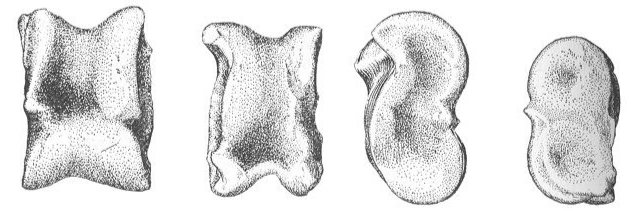
\includegraphics[width=\linewidth]{huesos}}
     \caption{Astrágalos, los predecesores de los dados}\label{Fig:huesos}
   \end{minipage}
\end{figure}

Hoy en día, las apuestas representan uno de los negocios más redituables del mundo. En 2013, se estimó que las ganancias brutas de esta industria sumaron más de cuatroscientos cuarenta mil millones de dólares\footnote{Acorde a la empresa de Inteligencia de Mercado ``H2 Gambling Capital'' \cite{economistHouseWins}.}. Como se puede observar en la figura~\ref{Fig:gasto-apuestas}, Estados Unidos encabeza la lista como el país que más gasta en apuestas, seguido por China. También se advierte que los residentes de Australia y Singapur apuestan mucho más agresivamente que los de cualquier otro país. Para terminar, en esta misma gráfica se estima que para el 2018 el gasto en apuestas será de más de quinientos mil millones de dólares.


\begin{figure}[!htb]\centering
   \begin {minipage}{0.85\textwidth}
     \frame{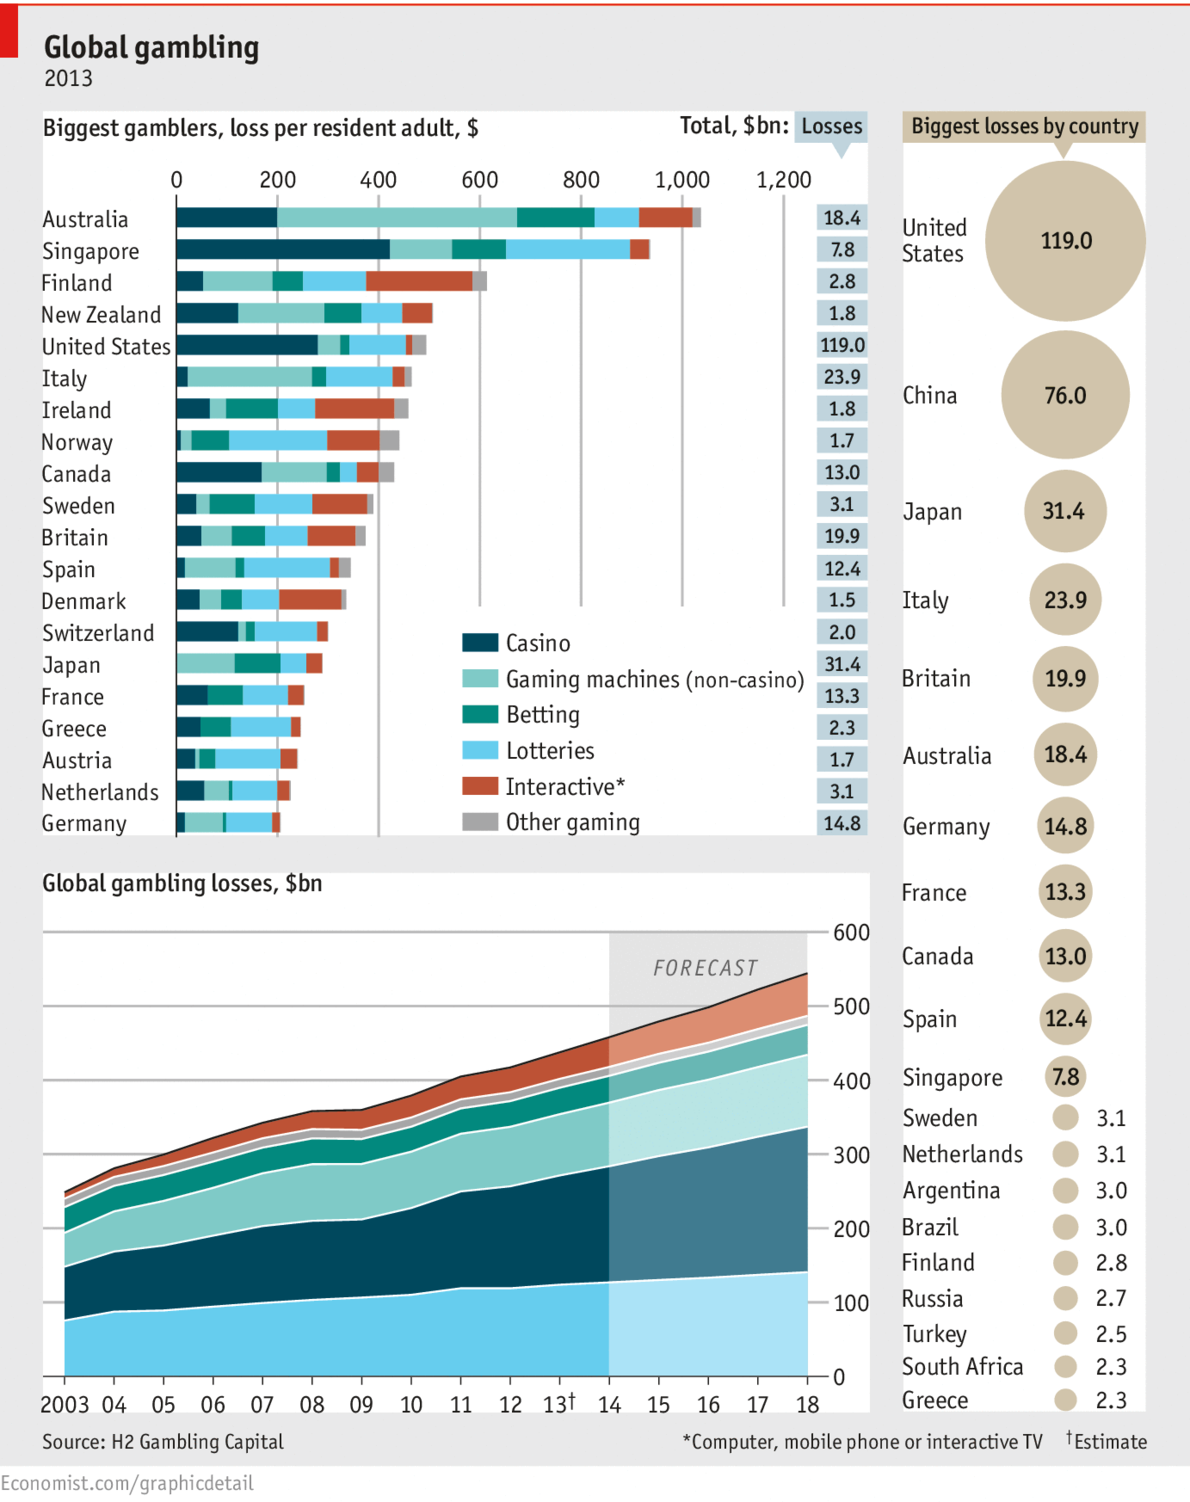
\includegraphics[width=\linewidth]{apuestas}}
     \caption{Miles de millones de dólares en apuestas}\label{Fig:gasto-apuestas}
   \end{minipage}
\end{figure}

Con estos datos, la relevancia de la industria de las apuestas en el mundo se vuelve evidente.  Ahora, abordando el ámbito de apuestas en línea, la firma KPMG \cite{kpmgOnlineGaming} presenta datos más focalizados; a pesar de la falta de regulación y las leyes en contra de los casinos en línea, el mercado global de apuestas en línea creció un cuarenta y dos por ciento de 2008 (Veintún mil doscientos millones de dólares) a 2012 (Treinta mil millones de dólares), este crecimiento es notablemente superior al quince por ciento que se propuso para el crecimiento del total de la industria de apuestas para el mismo periodo.

Específicamente en Estados Unidos, Goldman Sachs valoró en 2009 que el mercado de apuestas en línea en caso de ser legalizado\footnote{El ``Unlawful Internet Gambling Enforcement Act of 2006'' (UIGEA)  prohíbe a los bancos y a las compañías de tarjetas de credito procesar cargos relacionados a casinos en línea. Según Alexander, G. \cite{alexander2008us} las cuatro preocupaciones federales principales detrás de este acto son: Primero, el internet provee un acceso fácil a las apuestas, estoy podría exacerbar las tentaciones que enfrentan los apostadores compulsivos. Segundo, es muy complicado verificar la mayoría de edad a través de un sitio de apuestas. Tercero, los casinos en linea tienen un incentivo para defraudar a los usuarios gracias a la falta de regulación de la industria. Y cuarto, dado el volumen, la velocidad, el alcance internacional de la transacciones realizadas en internet y el alto nivel de anonimidad que tienen los operadores de casinos electrónicos; los oficiales federales creen que las apuestas en línea son particularmente suceptibles al lavado de dinero.} podría valer hasta doce mil millones de dólares \cite{goldmanParty}.En este mismo documento de KPMG \cite{kpmgOnlineGaming}, México se propone como un mercado potencialmente lucrativo. Una de las principales razones es la legislación que permite el juego en línea\footnote{En 2004, la Ley Federal de Juegos con Apuestas y Sorteos permitió y reguló los Juegos en Línea.}. La otra razón, el valor del mercado mexicano del juego en línea se estima en cuatro mil seiscientos millones de dólares \cite{yogonet}.

 \section{La casa siempre gana}



%Que no les gustó mi "INSPIRATIONAL QUOTE"
\begin{chapquote}{Adam Smith, \textit{Filósofo} \cite{smith1963wealth}}
	``No hay proposición más cierta en matemáticas que la siguiente: Entre más boletos [de lotería] compre, más probabilidades tiene de ser un perdedor. Compre todos los boletos de la lotería y pierda con certeza; cuanto más boletos compre, más cerca estará de esta certeza''
\end{chapquote}

%A ver así:
% \begin{savequote}[0.55\linewidth]
% ``No hay proposición más cierta en matemáticas que la siguiente: Entre más boletos [de lotería] compre, más probabilidades tiene de ser un perdedor. Compre todos los boletos de la lotería y pierda con certeza; cuanto más boletos compre, más cerca estará de esta certeza''
% \qauthor{Adam Smith, \textit{Filósofo} \cite{smith1963wealth}}
% \end{savequote}
% ok....  no jaló...


El principio básico detrás de un casino es muy sencillo: \emph{la ventaja de la casa}. Cada uno de los juegos que ofrece el casino tiene detrás un robusto sustento matemático que, a pesar de hacerlos aparentar como juegos justos, le confiere a la casa una ventaja porcentual sobre el conjunto de jugadores. Al final del día, esta ventaja y la ley de los grandes números, le garantizan a los casinos que a largo plazo tendrán suficientes ganancias para subsistir, mantener su operación y gozar de utilidades sorprendentes. Sin embargo, no hay que olvidar que los fenomenos estudiados siguen siendo producto del azar, por lo que una buena racha de algunos ``Grandes Apostadores'' podría llegar a asustar aun a los dueños  más racionales de casinos \cite{hannum2005practical}.



Según Hannum \cite{hannum2005practical} hay dos grandes razones por las que la gente apuesta:

\begin{enumerate}
	\item \textbf{Entretenimiento.} Un individuo podría utilizar mil pesos para ir a un casino o a un concierto. Si la ventaja de la casa es muy grande y la persona pierde su dinero rápidamente, entonces la experiencia del entreteniminto del casino no sería apreciada por el jugador. Por el otro lado, si el casino logra entretener a la persona por una tarde mientras le regala bebidas y comida, entonces puede que este individuo repita la experiencia y nunca más asista a un concierto.
	\item \textbf{Cambio de Vida.} Si una persona ahorrara cien pesos semanalmente, al final del un año tendría cinco mil doscientos pesos. Pero si ese dinero lo gastara para comprar boletos de lotería, tendría la posibilidad de ganarse cuarenta millones de pesos. Claramente la probabilidad es muy cercana a cero; sin embargo, este gasto podría ser visto por esta persona como una única oportunidad para cambiar su vida.

\end{enumerate}

\emph{La ventaja de la casa}, se puede entender mejor analizando cada uno de los juegos que ofrece el casino y las probabilidades de ganar que tienen los jugadores. Tómese el juego de la ruleta americana\footnote{El juego de la ruleta americana consiste en 18 casillas rojas, 18 casillas negras y 2 casillas sin color sobre las cuales, al girar de manera aleatoria, cae una pelotita. Los jugadores apuestan sobre la posición final de la pelotita.}:
Al tener $38$ casillas, si un jugador apuesta sobre el color negro (i.e. que la pelotita caiga sobre alguna de las casillas negras) entonces se tiene que la probabilidad de que el jugador gane la apuesta es de:\\
\[p\{\text{La pelotita caiga en casilla negra}\} = \frac{\text{\# casillas negras}}{ \text{\# casillas totales}}  = \frac{18}{38}\]\\

Afortunadamente para la casa, hay $2$ casillas que no son color negro ni rojo, por lo que de las $38$ sólo $36$ casillas tienen estos colores. Entonces, la probabilidaad de que la pelotita evite estos colores es la siguiente:

\[p\{\text{La pelotita no caiga ni en casillas rojas ni en negras}\} =\] 
\[\frac{\text{\# casillas totales - (\# casillas rojas + \# casillas negras)}}{ \text{\# casillas totales}}  =\]
\[\frac{38-18-18}{38} = \frac{2}{38}  \]

Estos $\frac{2}{38}$ son la ventaja de la casa, ya que cuando un jugador apuesta al color negro en la ruleta y acierta, recibe la misma cantidad de dinero que podría perder. Sin embargo, apostó a ganar con una probabilidad de $\frac{18}{38}$, pero la probabilidad de perder la apuesta es igual a $1 - \frac{18}{38} = \frac{20}{38}$. Este detalle hace importante ver el valor esperado que tiene esta apuesta para el jugador:
\[E[\text{Apostar }k\text{ pesos al color negro}] = k  \cdot   p\{\text{La pelotita caiga en casilla negras}\} \]
\[- k  \cdot   p\{\text{La pelotita no caiga en casilla negra}\} = k \cdot \frac{18-20}{38}= - k \cdot \frac{2}{38}\]

Dado que siempre que se apuesta $k>0$, esto implica que:
\[E[\text{Apostar }k\text{ pesos al color negro}] = - k \cdot \frac{2}{38} < 0; \forall k \in \mathbb{N} \]
Este resultado quiere decir que a la larga el jugador \textbf{siempre} va a terminar perdiendo dinero.
En un principio, $\frac{2}{38}$ de probabilidad pareciera poco, pero al multiplicarlo por la gran cantidad de jugadores y apuestas que se realizan en los casinos el monto final se vuelve exorbitante.

Este sencillo ejercicio ejemplifica como todos los juegos que se tienen en los casinos ofrecen una ventaja para la casa. Es interesante mencionar, que aparte de los juegos de azar como la ruleta, hay juegos que obligan al jugador a tener cierta habilidad para no perder su dinero tan rápidamente, este es el caso de juegos como el Blackjack que le dan a la casa ventajas más pequeñas al enfrentarse a jugadores expertos. La ventaja de la casa sustenta las ganancias del casino, sin embargo calcular esta ventaja puede llegar a ser  complicado y requerir un análisis matemático mucho más sofisticado e incluso se puede llegar a necesitar programar el juego para correr simulaciones y estimar estas probabilidades.

\begin{table}[ht]
\centering
\resizebox{\textwidth}{!}{%
\begin{tabular}{|l|c|}
\hline
\textbf{Juego}                            & \textbf{Ventaja de la Casa} \\ \hline
Ruleta (con doble cero)                   & 5.3\%                       \\ \hline
Dados (pass/come)                         & 1.4\%                       \\ \hline
Dados (pass/come con momios dobles)       & 0.6\%                       \\ \hline
Blackjack - jugador promedio              & 2.0\%                       \\ \hline
Blackjack - 6 barajas, estrategia básica  & 0.5\%                       \\ \hline
Blackjack - una baraja, estrategia básica & 0.0\%                       \\ \hline
Baccarat (sin apuestas de empate)         & 1.2\%                       \\ \hline
Caribbean Stud                            & 5.2\%                       \\ \hline
Let It Ride                               & 3.5\%                       \\ \hline
Poker de tres cartas                      & 3.4\%                       \\ \hline
Pai Gow Poker (ante/play)                 & 2.5\%                       \\ \hline
Tragamonedas                              & 5\% - 10\%                  \\ \hline
Video Poker                               & 0.5\% - 3\%                 \\ \hline
Keno (promedio)                           & 27.0\%                      \\ \hline
\end{tabular}
}
\caption{Ventajas de la casa para juegos populares de casino \cite{hannum2005practical}}
\label{ventaja-casa}
\end{table}

Finalmente, aun sin la ventaja de la casa se deber recordar que existe un famoso problema y su corolario que garantizan que la casa siempre gane: \emph{La ruina del Jugador} \cite[p.~95-99]{ross2006first}. Este problema enfrentado por varios famosos matemáticos\footnote{Se dice que Blaise Pascal se lo planteó a Pierre Fermat en 1656 \cite{edwards1983pascal}. Después Fermat se lo replanteo a Christian Huygens en 1657 y finalmente James Bernoulli lo resolvió en su forma general como el problema de la ``Duración de Juego''. Fue publicado ocho años después de la muerte de Bernoulli en 1713 \cite[p.~98]{ross2006first}.} deja la siguiente lección: La probabilidad de un jugador perder todo su dinero es igual a  $p_1 = \frac{n_2}{n_1 + n_2}$ donde $p_1$ es la probabildad de ganar del jugador $1$ y $n_i$ es la cantidad de dinero que va a apostar el jugador $i$. Desafortunadamente, usualmente la casa tendrá más dinero para apostar que cualquier jugador, por lo que con esta fórmula la casa siempre gana\footnote{Ver demostración en el apéndice~\ref{chap:ruina}.}.


 \section{Mercados de apuestas deportivas}
 
 A diferencia de las máquinas tragamonedas y los juegos de mesa de los casinos, las apuestas deportivas tienen una gran ventaja para los apostadores: los resultados de los encuentros deportivos \textbf{no son completamente aleatorios,} ya que dependen en cierta medida del nivel de juego que tienen los equipos participantes. Hannum menciona en su libro \cite{hannum2005practical} : \emph{``La ventaja de la casa existe para casi todas las apuestas en un casino (ignorando las salas de Poker y las apuestas deportivas donde algunos pocos profesionales pueden vivir de de las apuestas)''}

 Existen dos grandes mercados en esta rama de las apuestas \cite{chung2010empirical}:
 \begin{itemize} 
 	\item \emph{Bookies.}\footnote{``Bookie'' proviene de la palabra en inglés ``bookmakers'' que en español se utiliza como: ``Corredor de apuestas''.} El corredor de apuestas analiza los diferentes resultados de un encuentro deportivo en función de los participantes. Con base en este análisis, el bookie publica un número (llamado \emph{``momio''}) para cada uno de los posibles desenlaces del partido. Este ``momio'' reprensenta la cantidad potencial de retorno de esa apuesta (incluída la cantidad de dinero arriesgada)\footnote{Por ejemplo, supongase que se apuestan cien dólares a favor del empate de un partido con un momio igual a $3.640$. En caso de que se ganara la apuesta, el jugador recibíria la cantidad de $(100)(3.640) = 364$ dólares. Sustrayendo los cien dólares que apostó, su ganancia neta sería de $264$ dólares.}. El bookie recibe apuestas sobre estos momios y cobra una comisión por cada operación recibida. 
 	\item \emph{Sistema parimutual.} En este mercado no existen  corredores, ni momios. El pago que reciben los jugadores depende de la cantidad de dinero recopilada por todas las apuestas recibidas. Por lo tanto, las ganancias de los jugadores no están determinadas hasta que todas las apuestas se reciben\footnote{Las afamadas ``quinielas'' son un tipo de apuesta de mercado parimutual.}.
 	\end{itemize}

 Aunque la eficiencia\footnote{Fama, E \cite{fama1998market} sugiere que la eficiencia de mercado es cuando los precios reflejan completamente toda la información disponible de una acción en particular.} de estos mercados no es un tema que se profundize en esta tesis, es interesante mencionar que ha sido  muy cuestionada. Sauer \cite{sauer1998economics} y Williams \cite{williams1999information} critican varias de sus anomalías, por ejemplo hay un problema interesante en la eficiencia del mercado de las apuestas de los bookies conocido como: Sesgo del \emph{``favorite - long shot''.} Estos autores explican que las apuestas a los equipos favoritos generan un mayor retorno de dinero en comparación con el retorno generado por las apuestas a equipos cuyas probabilidades de ganar son mucho menores (``longshot bets''). Incluso se han realizado varios estudios proponiendo un nuevo mercado de tipo ``doble subasta'' que consiste en tener compradores y vendedores proponiendo los precios de la apuesta, cuando dos de ellos coinciden, se lleva acabo la transacción. Referirse a Ozgit\cite{ozgit2005posted}.

 El mercado de estudio de este trabajo es el de los ``bookies'' o corredores de apuestas. Sin embargo, bajo las condiciones adecuadas la asesoría de apuestas podría ayudar a los jugadores en el mercado parimutual. Por ejemplo, en una apuesta entre compañeros del trabajo el usuario del sistema podría indagar la apuesta realizada por cada uno de los participantes y conocer la cantidad de retorno que tiene de cada uno de los resultados. Si el sistema de Egobets le recomendara realizar esta apuesta en particular, bastaría verificar que el retorno del pago sea mejor que el pago que realizan las casas de apuestas en general. Realizando esta acción sistemáticamente se podrían conseguir buenas ganancias sobre los partidos que realmente vale la pena apostar en cada jornada.

 Sin importar el mercado, es importante que recordar el hecho de que las probabilidades reales que tienen los distintos resultados de cualquier partido \textbf{son desconocidas}. Por lo que los ``bookies'' contratan a empresas consultoras, o designan un área de la compañía para calcular los momios que se publican en el mercado. Este punto es básico en la creación de sistemas como Egobets, ya que el hecho de que las probabilidades sean desconocidas permite que Egobets busque estimar probabilidades mucho más cercanas a las reales. Al minimizar el error de estimación, que tienen las probabilidades sugeridas por las casas de apuestas, se pueden encontrar apuestas cuyo retorno sería mayor al que realmente debería ser. Y como se verá en la siguiente sección, este error de estimación siempre existirá, debido a que los momios publicados por las casas de apuestas no buscan reflejar las probabilidades reales de los resultados de los partidos.

 Para concluir esta sección, se tiene que una ventaja más para los apostadores de eventos deportivos: si los bookies establecen mal sus momios\footnote{La cantidad de dinero que pagan las apuestas a eventos completamente aleatorios, como los son los juegos dentro de los casinos, se pueden calcular explícitamente. Por lo que la única manera de que una de estas apuestas tuviera valor esperado positivo sería si se cometieron errores en los cálculos.}, entonces ciertos jugadores pueden llegar a tener valores esperados positivos en sus apuestas y con esto la casa podría llegar a perder mucho dinero, incluso a largo plazo (como se verá en la siguiente sección). Procédase a la siguiente sección para conocer los orígenes de los momios y las condiciones que permiten a los bookies ganar dinero con ellos.
 
 \section{Bookies y momios}
 Para generar los momios, las casas de apuesta realizan estudios minuciosos de mercado y de los deportes en sí mismos. Sin embargo, Levitt \cite{levitt2004gambling} menciona tres escenarios que permitirían a los bookies generar ganancias:
 \begin{enumerate}
 	\item \textbf{Encontrar el precio de equilibrio.} Los bookies buscan predecir los momios\footnote{Antes del partido estos momios pueden llegar a tener ajustes tipicamente pequeños y relativamente infrecuentes.} que igualen el precio de equilibrio del mercado de apuestas. Es decir, se buscan los momios que equilibran la cantidad de dinero en cada lado de la apuesta. Esto implica que la diferencia de dinero entre todas las apuestas es igual a cero. Por lo que sin importar quien gane el partido, el bookie cobrará su comisión de las apuestas intacta y no tendrá deudas en ninguna de las apuestas.
	
 	\item \textbf{Predecir los resultados del partido.} Si el bookie fuera sistemáticamente mejor en predecir los resultados de los partidos, entonces podría publicar el momio ``correcto'' del partido (i.e. el momio que equilibra la probabilidad de que una apuesta en cualquiera de los resultados gane). Aunque la cantidad de dinero no estaría equilibrada, en promedio el bookie ganaría la comisión cobrada a los jugadores. Nótese que a diferencia del primer escenario, en este esquema existe un riesgo enorme al que se exponen las casas de apuestas. Si llegaran a fijar un momio muy alejado del precio de equilibro del mercado, entonces podría darse el caso de que la cantidad de dinero a pagar a los ganadores de la apuesta sea mayor a la cantidad de dinero recaudada por las apuestas complementarias, lo que podría significar pérdidas millonarias para el bookie\footnote{Levitt \cite{levitt2004gambling} cuenta el ejemplo del Epson Derby de 1946, donde los momios fueron errados y la mitad de todas las casas de apuestas británicas se fueron a bancarrota.}.
	
	
 	\item \textbf{Predecir los resultados y encontrar el precio de equilibrio.} Si el bookie es mejor que los jugadores prediciendo el resultado de los partidos y también puede encontar el precio de equilibrio, entonces podría con esta información mejorar sus ganacias esperadas al publicar un momio ``equivocado'' de tal manera que el momio (precio) de equilibrio quede posicionado donde sus ganancias se incrementen. Ahora, hay ciertas restricciones en cuanto a la distancia a la que puede quedar posicionado el momio ``equivocado'', ya que pueden existir jugadores que conozcan el momio ``correcto'' por lo que entre mayor sea esta distancia podría generar mayores ganancias para estos jugadores. Por ejemplo, supongase el siguiente caso extremo: Se disputa un partido entre los equipos $A$ y $B$, el equipo $B$ es el favorito para ganar. Es por esto que la casa de apuestas arregló que el partido lo gane el equipo $A$. El bookie conoce que la probabilidad de que el equipo $A$ gane el partido es $1$, es por esto que fija los momios más competitivos del mercado a favor del equipo $B$ y a favor del empate, mientras que el momio a favor del equipo $A$ lo presenta mucho menos competitivo que el resto del mercado. Con estas acciones, la casa de apuestas maximiza las apuestas recibidas en contra del equipo $A$ y minimiza las apuestas a favor del equipo $A$ dado que las otras casas de apuestas pagan mucho mejor este resultado. Ahora, si los momios fueran absurdamente buenos en contra del equipo $A$ ciertos apostadores podrían intuir que la casa de apuestas sabe algo que los demás no saben y podrían apostar cantidades exorbitantes a favor del equipo $A$.
 \end{enumerate}


 De estos tres escenarios, Levitt \cite{levitt2004gambling} examina de un bookie en línea, veinte mil apuestas de doscientos ochenta y cinco jugadores para los partidos de la NFL\footnote{La liga de futbol americano más popular: National Football League.}. Esto fue lo que encontró:
 \begin{itemize}
 	\item A pesar de ser un estudio para una sola casa de apuestas, sugiere que se pueden generalizar ya que casi todas las casas ofrecieron casi los mismos momios para los mismos partidos
 	\item El bookie no parece buscar el precio de equilibrio del mercado. Acorde a los resultados en casi la mitad de todos los juegos al menos dos tercios de las operaciones caen en un solo lado de la apuesta.
 	\item El bookie parece colocar precios estratégicamente para explotar los sesgos de los apostadores. Es decir, los jugadores parecen tener un sesgo sistemático hacia los equipos favoritos y, en menor medida, hacia los equipos visitantes. En consecuencia, el bookie logró atraer mayor atención a partidos donde estos equipos no tuvieron buenas actuaciones; estos precios lograron elevar las ganancias hasta un veinte por más que con lo que hubieran obtenido en el primer escenario.
 	\item Hay poca evidencia de que existan jugadores que hayan sido capaces de vencer a los bookies sistemáticamente.
  \end{itemize}
 
 Estas conclusiones indican que, al menos en el deporte del futbol americano, las casas de apuestas buscan siempre tener mayores ganancias y que podrían estar usando el tercer escenario descrito previamente. 
 
 \section{Margen de los bookies}
 En la sección anterior se habló de un momio como el número que indica la cantidad de dinero que obtiene un jugador al ganar una apuesta. Sin embargo, para entender el origen de este número hay que analizar las probabilidades de que ocurra el evento y la cantidad de dinero que se apuesta para sus diferentes resultados.
 
 Ya que el objeto de estudio central de esta tesis toma lugar en el deporte del futbol, analícese la pregunta más recurrente de un partido de futbol: \emph{¿Qué equipo va a ganar este partido?}

 La respuesta tiene $3$ posibilidades:
 \begin{enumerate}
 	\item El partido lo gana el equipo de casa.
 	\item Es un empate.
 	\item El partido lo gana el equipo visitante.
 \end{enumerate}
 En un principio se pudiera pensar que los tres eventos son equiprobables, pero como se mencionó en la sección anterior esto resulta imposible por muchísimas razones, como por ejemplo: ser el equipo visitante conlleva una desventaja importante en el desempeño del partido (Ver \cite{roffe2007crisis}), o la desventaja de tener a los jugadores estrella lesionados. Bueno, inclusive las condiciones climáticas (altitud, tipo de pasto, lluvia) durante el partido pueden ser determinantes para el resultado final. Piénsese incluso el escenario donde ambos equipos fueran igual de buenos en todos los aspectos. En este escenario, la probabilidad de empate sería mayor que las otras dos. Sin embargo, estas razones no son (tampoco) suficientes para calcular los resultados de los partidos de manera determinística. Gracias a estas particularidades es que el estudio de este mercado de apuestas se vuelve tan interesante.
 
 Sea $m_i$ el momio que propone el bookie para que los jugadores apuesten a que se cumpla el evento $i$. Entonces, se define el momio de la siguiente manera:
 \[m_i = \frac{1}{1 - \hat{p_i}}\]
 Donde $\hat{p_i}$ es la probabilidad estimada que tiene el bookie de que suceda el evento $i$\footnote{Otros deportes tienen diferentes tipos de momios y su definición varía dependiendo del tipo de apuesta, se puede leer más de ellos en \cite{ignatin1984sports}.}

 Ahora, tómese de ejemplo el siguiente partido con los siguientes momios:
 \begin{itemize}

 \item \textbf{Cagliari Vs Juventus.}
 	\begin{itemize}
 		\item \textbf{9.290} Gana local (Cagliari)
 		\item \textbf{1.423} Empate.
 		\item \textbf{4.760} Gana visitante (Juventus)
 	\end{itemize}
 \end{itemize}

 Con estos momios se pueden calcular las ``probabilidades estimadas por el bookie'':
 \[\hat{p_L} = 1 - \frac{1}{9.290} \approx 0.107643...\] 
 \[\hat{p_E} = 1 - \frac{1}{1.423} \approx 0.702741...\]
 \[\hat{p_V} = 1 - \frac{1}{4.760} \approx 0.210084...\]
 Donde $\hat{p_L}$ es la probabilidad estimada por la casa de apuestas de que gane el equipo local, $\hat{p_E}$ es la probabilidad de que el partido termine en empate y $\hat{p_V}$ es la probabilidad de que gane el equipo visitante.
 Estas probabilidades estimadas proponen que el escenario más probable es un empate, después la victoria del Juventus y finalmente la victoria del Cagliari. Curiosamente en este ejemplo, se puede ver que aunque el equipo Cagliari es local, se enfrenta a un adversario que puede contra la desventaja de ser visitante.

 Uno de los teoremas básicos de la probabilidad, dice que la suma de las probabilidades de todos los resultados del evento debe sumar uno \cite{ross2006first}. Sin embargo, en el caso de los bookies, las probabilidades estimadas exceden la unidad. Este excedente, es la conocida ``Ventaja de la Casa''.

 Sea $\mathcal{O}$ el conjunto de todas las opciones sobre las que un jugador puede apostar para cierto evento\footnote{Para el caso de las apuestas sobre los resultados de los partidos, se tiene que: $\mathcal{O} = \{\text{Apostar a que gane local}, \text{Apostar al empate}, \text{Apostar a que gane visitante}\}$.}.
 \[\text{Ventaja de la casa} =  \left(\sum_{i \in \mathcal{O}}{\left(1 - \frac{1}{\text{Momio de la opción } i}\right)}\right) - 1\] 

 Siguiendo con el ejemplo, se tiene que la ventaja de la casa de este bookie para esta apuesta en particular es:
 \[\text{Ventaja de la casa} = \hat{p_L} + \hat{p_E} + \hat{p_V} - 1 \approx 0.020467\]

 Este $2.046\%$ es el punto de partida que la casa quiere obtener en ganancias. Sin embargo, si la casa conociera las probabilidades reales de los resultados del partido, entonces podría (por ejemplo) presentar para ese partido al equipo visitante (Juventus) como la mejor opción para la apuesta, cuando en realidad no lo es. Este tipo de técnicas aplicadas sistematicamente pueden ayudar al bookie a obtener ingresos mayores a largo plazo.

 La información obtenida en esta sección aumenta las esperanzas de que sistemas como Egobets, que funcionan al aprovecharse de los momios ``equivocados'' propuestos por las casas de apuestas, pudieran llegar a funcionar satisfactoriamente.
 

%  \section{Ligas europeas de futbol}
% El nivel de juego de los clubes europeos es sorprendente, tanto en la cancha como fuera de ella los Clubes de futbol de las ligas europeas hacen las cosas mejor que ningún otro. Ofrecen partidos de alta calidad, con jugadas complejas y rápidas que proveen de un espectáculo como ningún otro. Además de que la infraestructura, adminsitración y los recursos financieros con los que cuentan son envidiables. Y es por estos motivos que sus niveles de audiencia y la cantidad de sus fanáticos han llegado a niveles impresionantes. Las ligas europeas son en el mundo del futbol: \emph{El modelo a seguir.}
%
%
%
% Además de todas las cualidades con las que cuentan estas ligas, se tiene una premisa muy interesante incita el enfoque en ellas: La consistencia que tienen los equipos más populares de cada liga para conseguir victorias sobre los equipos más modestos y su habilidad para siempre permanecer en los mejores lugares de la tabla de posiciones.
%
% \section{Ingeniería de Software}
%  \section{Contribuyendo al Internet con un granito de arena}
% La era de la información nos golpeo tan fuerte, que ahora es imposible la vida sin nuestros sistemas de información y nuestros dispositivos de conexión. Gracias a las computadoras y las redes, se ha redefinido nuestra imaginación, se ha creado un espacio que expande nuestra mente y nuestra capacidad, nuestras barreras se han alejado más y ahora nuestra conciencia como especie humana, crece en tasas inimaginables. Los monopolios de la información se han ido disolviendo, permitiendo a la sociedad una mayor participación y voz.
%
% Internet es un organismo vivo y hambriento, con el que convivimos de manera simbiótica y nos une como especie. Es un espacio de comunicación y entendimiento. Nunca pudo haber existido algo más majestuoso y poderoso. La verdadera trascendencia del ser, vendrá con la evolución de la conciencia de la sociedad.
%
% Con esta idea en mente fue diseñado y desarrollado Egobets, un sistema que aporta a la comunidad en internet información últil para la toma de mejores decisiones. Y a su vez, esta información, proviene del procesamiento de varias fuentes de información que otros aportan al internet. El ideal detrás: un conjunto de círculos virtuosos que pongan al alcance de cualquier persona la información más precisa y útil acerca de cualquier tema que se pueda pensar.
%
%  \section{Computación en la Nube}
%
% El sistema usa la nube para ofrecer sus servicio a los usuarios, se puede decir que el software corre en un esquema tipo ``SaaS''\footnote{Software as a Service. ``Es el más conocido de los niveles de cómputo en la nube. El SaaS es un modelo de distribución de software que proporciona a los clientes el acceso a éste a través de la red (generalmente Internet). De esta forma, ellos no tienen que preocuparse de la configuración, implementación o mantenimiento de las aplicaciones, ya que todas estas labores se vuelven responsabilidad del proveedor. Las aplicaciones distribuidas a través de un modelo de Software como Servicio pueden llegar a cualquier empresa sin importar su tamaño o ubicación geográfica.'' \cite{computoNube}.}, esto implica que el usuario simplemente ingresa a su cuenta en un navegador de internet y puede ver las asesorías para sus apuestas.
% Del artículo ``Cómputo en Nube: Ventajas y Desventajas'' de Martínez y Gutiérrez \cite{computoNube}  se retoman las siguentes ventajas de este paradigma:
% \begin{itemize}
% 	\item \textbf{Costos.} Podría ser la ventaja más atractiva que presenta el cómputo en la nube, y si no lo es, al menos es la más evidente de todas las que ofrece esta tecnología. Al dejar la responsabilidad de la implementación de la infraestructura al proveedor, el cliente no tiene que preocuparse por comprar equipos de cómputo, capacitar personal para la configuración y mantenimiento de éstos, y en algunos casos, por el desarrollo del software. Además el usuario de estos servicios únicamente paga por los recursos que utiliza, permitiéndole diseñar un plan de pago normalmente a partir del tiempo en que éste se utiliza (memoria, procesamiento, almacenamiento).
%
% 	\item \textbf{Competitividad.} Al no tener que adquirir equipos costosos, las pequeñas empresas pueden tener acceso a las más nuevas tecnologías a precios a su alcance pagando únicamente por consumo. De este modo las organizaciones de cualquier tipo podrían competir en igualdad de condiciones en áreas de TI con empresas de cualquier tamaño. La ventaja competitiva no está en aquel que tiene los recursos de cómputo sino en quien los emplea mejor.
%
% 	\item \textbf{Disponibilidad.} El proveedor está obligado a garantizar que el servicio siempre esté disponible para el cliente. En este sentido, la virtualización juega un papel fundamental, ya que el proveedor puede hacer uso de esta tecnología para diseñar una infraestructura redundante que le permita ofrecer un servicio constante de acuerdo a las especificaciones del cliente.
%
%
% 	\item \textbf{Abstracción de la parte técnica.} Como se mencionó al hablar de costos, el cómputo en la nube permite al cliente la posibilidad de olvidarse de la implementación, configuración y mantenimiento de equipos; transfiriendo esta responsabilidad al proveedor del servicio.
%
% 	\item \textbf{Acceso desde cualquier punto geográfico.} El uso de las aplicaciones diseñadas sobre el paradigma del cómputo en la nube puede ser accesible desde cualquier equipo de cómputo en el mundo que esté conectado a Internet. El acceso normalmente se hace desde un navegador web, lo que permite a la aplicación ser utilizada no únicamente desde una computadora de escritorio o una computadora portátil, sino que va más allá, permitiendo al usuario hacer uso de la aplicación incluso desde dispositivos móviles como smartphones.
%
% 	\item \textbf{Escalabilidad.} El cliente no tiene que preocuparse por actualizar el equipo de cómputo sobre el que se está corriendo la aplicación que utiliza, ni tampoco por la actualización de sistemas operativos o instalación de parches de seguridad, ya que es obligación del proveedor del servicio realizar este tipo de actualizaciones. Además, éstas son transparentes para el cliente, por lo que la aplicación debe de continuar disponible para el usuario en todo momento aún cuando se esté realizando el proceso de actualización del lado del proveedor. Las actualizaciones y nuevas funcionalidades son instaladas prácticamente de manera inmediata.
%
% 	\item \textbf{Disponibilidad.} El proveedor está obligado a garantizar que el servicio siempre esté disponible para el cliente. En este sentido, la virtualización juega un papel fundamental, ya que el proveedor puede hacer uso de esta tecnología para diseñar una infraestructura redundante que le permita ofrecer un servicio constante de acuerdo a las especificaciones del cliente.
%
% \end{itemize}
%
% Estas ventajas fueron más que suficientes para realizar el desarrollo en la nube. Además de que la realización de un nuevo prouecto utilizando nuevas tecnologías siempre aporta mayor emoción y reto al desarrollo de software.
%
% Patrones de diseño
%
% Bases de Datos no Relacionales
%
% Lenguajes:
% PHP
% js
% fortran
%
%









 %Panorama general de apuestas
\graphicspath{{/Users/brunomedina/Dropbox/Tesis-Egobets/egobets-notas/resources/}}

\chapter{Sistematización de las apuestas}
\label{chap:mate}

% En este capítulo se presentan, sin entrar al detalle técnico, los resultados comprobables de las teorías que proporcionan las probabilidades de los resultados de los partidos y las predicciones de sus resultados. De igual manera se destaca la importancia de un sistema de reservas para optimizar las tasas de crecimiento de la cantidad de dinero dedicada a las apuestas. Finalmente se retoman estos conceptos y se detalla el algoritmo que utiliza Egobets para la generación de las recomendaciones de apuestas.

En este capítulo se detallan las variables y los pasos que tiene el método utilizado por el sistema de Egobets para proveer a sus usuarios de una asesoría de apuestas personalizada. En la primera parte del capítulo, a modo de introducción, se discutirá si es posible modelar de manera matemática un partido de futbol con la finalidad de predecir su resultado. Además, en esta misma sección se explica como el afamado criterio de Kelly introduce la noción de un sistema de reservas y busca optimizar la ganancia esperada en función de restringir la fracción de dinero a invertir en cada partido.

\section{Antecendetes y evidencia a favor}
\label{sec:evidencia}

Esta tesis no busca predecir los resultados de los partidos de futbol, sin embargo es importante mostrar que esto se puede lograr y que más de algún autor ha encontrado maneras teóricas eficientes de hacerlo. De igual manera, se explica (sin entrar a detalle) uno de los modelos más utilizados en este ámbito: la Poisson bivariada. Esto ayuda al lector a comprender cuales son las variables que parecen afectar más los resultados y le permite tener una mejor noción de lo que puede ser una buena apuesta.

Después de exhibir el modelo, se presentan dos ejemplos concretos de estrategias de apuestas: la estrategia simple (e intuitiva) y la estrategia de Kelly. En particular, Kelly le da al problema un paradigma financiero y abre el camino a buscar apuestas que no arriesguen todo el capital del jugador. Esta idea será retomada en la siguiente sección para el sistema de reservas.

\subsection{Modelar un partido de futbol}
\label{subsec:modelo}


% El tema central de esta tesis no es la predicción de resultados de futbol principal si no la generación automatizada de recomendaciones de apuestas, por este motivo y para evitar cuestiones de plagios del modelo predictivo de Egobets, en este apartado no se entrarán en los detalles de la implementación, solamente se mostrarán las teorías los modelos matemáticos prácticos que permiten predecir los resultados de los partidos de futbol sobre los que se basa Egobets. Los resultados de los estudios analizados en esta sección son suficientes para evidenciar la existencia de un conjunto de probabilidades y resultados estimados que permitan desarrollar una estrategia de apuestas capaz de generar un valor esperado positivo.
%


Dixon y Coles (1997) \cite{dixon1997modelling} en su contribución, mencionan algunas propiedades deseables en un modelo de futbol:
\begin{itemize}
	\item Se deben considerar las habilidades de ambos equipos en un partido.
	\item Se debe dar lugar a la ventaja observada que tienen los equipos al jugar en casa.
	\item La medida más razonable de la habilidad de un equipo debe basarse en el desempeño de sus últimos juegos.
	\item La habilidad de un equipo, por la naturaleza del futbol, se comprende como la composición de la habilidad de ataque (anotar goles) y la habilidad de defensa (no recibir goles).
	\item Al presentar el desempeño de un equipo en sus recientes resultados, se deberá tomar en cuenta la habilidad de los equipos contra los cuales ha jugado.
\end{itemize}


 \subsubsection{Modelo de Poisson bivariada}
 \label{subsubsec:bivariate-poisson}

Koopman y Lit (2013) \cite{koopman2013dynamic} proponen el siguiente modelado de los partidos de futbol.
\begin{itemize}

	\item Supóngase que se tienen $J$ equipos en una liga donde cada semana juegan todos los equipos.

	\item Los equipos juegan dos veces contra todos los demás equipos, una vez de visitante y otra de local.
	\item Tómese el par $(X_{it},Y_{jt})$ como la cantidad de goles del partido. 
	\begin{itemize}
	
		\item $X_{it}$ es el número no negativo de goles anotados por el equipo local $i$ en la semana $t$.
		\item $Y_{jt}$ corresponde al número de goles anotados por el equipo visitante $j$ en esa misma semana $t$.
	\end{itemize}
		
		Para $i\neq j = 1, ...,J$ y $t=1,...,n$, con $n$ la cantida de semanas con partidos jugados (es decir que tienen datos).
\end{itemize}

\paragraph{Distribución Poisson Bivariada} % (fold)
\label{par:distribucion_poisson_bivariada}
Cada par de cuentas $(X,Y) = (X_{it},Y_{jt})$ se genera de una distribución Poisson bivariada con la siguiente función de masa de probabilidad:
 
 \[p(X,Y;\lambda_x,\lambda_y,\gamma) =\]
  \[e^{(-\lambda_x-\lambda_y-\gamma)}\frac{\lambda^X_x}{X!}\frac{\lambda^Y_y}{Y!}\sum_{k=0}^{min(X,Y)}\left(\frac{X}{k}\right)\left(\frac{Y}{k}\right)k!\left(\frac{\gamma}{\lambda_x\lambda_y}\right)^k \]

 para $X = X_{it}$ y $Y = Y_{it}$.
 Con $\lambda_x$ y $\lambda_y$ coeficientes que reflejan la intensidad de goleo para $X$ (equipo) y $Y$ (visitante) respectivamente en la jornada $t$.
 Y con $\gamma$ siendo el coeficiente que mide la dependencia entre los goles anotados por el local y el visitante $(X,Y)$. 

 La notación corta se describe como\footnote{La definición que se presenta en este documento es propuesta por \cite{koopman2013dynamic}, sin embargo hay otras variantes de esta fórmula \cite{kocherlakota1992bivariate} y \cite{johnson1997discrete}}:
 \boldmath\[(X,Y) \sim BP(\lambda_x,\lambda_y,\gamma)\]\unboldmath 
 % paragraph distribucion_poisson_bivariada (end)
 

\paragraph{Valor Esperado, Varianza y Covarianza} % (fold)
\label{par:valor_esperado}
 \[E(X) = \mathrm{Var}(X) = \lambda_x + \gamma \text{, } E(X) = \mathrm{Var}(Y) = \lambda_y + \gamma\]
 
 \[\mathrm{Cov}(X,Y) = \gamma\]


 y el coeficiente de correlación entre $X$ y $Y$ está dado por:
 \[\rho = \frac{\gamma}{\sqrt{(\lambda_x+\gamma)(\lambda_y+\gamma)}}\]
 
% paragraph valor_esperado (end)




\subsubsection{Intuición detrás del modelo}
\label{subsubsec:intuicion}
 El resultado de restar los goles del local menos los del visitante $X-Y$ determina si el partido fue ganado, perdido o empatado por el equipo de casa\footnote{La variable $X-Y$ tiene una distribución de probabilidad discreta conocida como: Skellman y conlleva muchas propiedades descritas en Skellman (1946) \cite{skellam1946frequency}}. Esta noción de modelar los partidos en función de la cantidad de goles de cada equipo se retoma del artículo de Maher (1982) \cite{maher1982modelling}, en el cual se narra que la posesión del balón origina la oportunidad de atacar y anotar un gol. La probabilidad de que un ataque resulte en gol puede ser pequeña, pero se debe recordar que son muchas las veces que el equipo tiene la posesión de la pelota durante el encuentro. Entonces, si se considera que la probabilidad de anotar en cada ataque es independiente, se puede afirmar que el número de goles se pueden modelar bajo una distribución Binomial. Es por esto, que se puede aplicar la aproximación Poisson.
 
 Ahora el resultado del partido y la cantidad de goles, dependen de los parámetros $\lambda_x$, $\lambda_y$ y $\gamma$ de la distribución. En concreto, obsérvese que $\lambda_x$ (que como ya se mencionó, depende de $X = X_{it}$) es el coeficiente que determina las anotaciones que tendrá el equipo local $i$ en el partido de la semana $t$ sobre el equipo $j$. Es decir, $\lambda_x$ depende de la habilidad (tanto ofensiva como defensiva) del equipo $i$ al jugar contra el equipo visitante $j$. De manera análoga, $\lambda_y$ dependerá en este partido de las fortalezas del equipo visitante $j$ contra el equipo $i$.
 Esto quiere decir que las $\lambda$'s del modelo van en función de cada equipo según su fortaleza ofensiva y defensiva contra cada adversario, siendo local o visitante. Y estas, son justamente las propiedades son las listadas en la sección~\ref{subsec:modelo} propuestas Dixon y Coles (1997) \cite{dixon1997modelling}.
 
 Por otra parte, el parámetro $\gamma$ está definido para los empates. Al aumentar $\gamma$, aumenta la dependencia entre la cantidad de goles obtenidos por el local y por el visitante, Maher (1982) lo notó en su estudio \cite{maher1982modelling} y propuso este coeficiente para ajustar los casos donde simplemente no había goles. A su vez, Koopman (2013) \cite{koopman2013dynamic} menciona que a conforme aumentaba $\gamma$, aumentaban la cantidad de empates generados por el modelo\footnote{Un valor de $\gamma = 0.05$ con $\lambda_x =\lambda_y = 1$  aumentaba los empates $3.3\%$ en comparación de cuando $\gamma = 0$. Y cuando $\gamma = 0.20$ el aumento en la cantidad de empates era del $14\%$ \cite{koopman2013dynamic}}.  
 
 
 % En su artículo \cite{dixon1997modelling}, consideran la doble Poisson con un parámetro de dependencia que se estima junto con los otros parámetros. Sugieren que la suposición de independencia entre los goles de los equipos, tiene cabida en los partidos con resultados: 0-0, 1-0, 0-1 y 1-1\footnote{Karlis y Ntzoufras (2003) \cite{karlis2003analysis} sugieren que la predicción de empates mejora si se considera un parámetro de dependencia (incluso aunque sea pequeño)}. Además, agregan al modelo una función que pondera los partidos con el fin de ``diluir'' los efectos de los partidos más lejanos.

 % Después, Rue y Salvensen (2000) \cite{rue2000prediction} retoman el análisis de Dixon y Coles \cite{dixon1997modelling} y lo adoptan en un modelo dinámico lineal generalizado y adoptan un procedimiento de estimación Bayesiano para estudiar las propiedades de los equipos sobre un tiempo variable\footnote{En su análisis empírico truncan la cantidad de goles a no más de cinco, consideran que esos marcadores no proveen mayor información acerca del ataque y defensa de un equipo.}. De igual manera, Crowder, Dixon, Ledford, and Robinson (2002) \cite{crowder2002dynamic} representan el modelo de Dixon y Coles \cite{dixon1997modelling} como un espacio de estados no Gaussiano con fuerzas de ataque y defensa variables en el tiempo, la estimación se realiza utilizando métodos de aproximación por su alto costo computacional. Adicionalmente, Ord, Fernandes, and Harvey (1993) \cite{ord1993time} presentan una extensión multivariada de un modelo de daros de conteo dinámico Bayesiano para el análisis y predicción del número de do goles marcados por algún equipo.

 % Finalmente, Koopman y Lit (2013) \cite{koopman2013dynamic} retoman todas estas ideas y presentan un modelo Poisson bivariado con ataque y defensa como variables estocásticas en función del tiempo. 
 
 % Maher en 1982 \cite{maher1982modelling} describió la intuición detrás del modelado de un partido de futbol. Los goles anotados por un equipo en un partido pudieran ser modelados por una variable Poisson, la posesión es un aspecto importante del futbol ya que cada vez que un equipo tiene la pelota tiene la oportunidad de atacar y anotar. La probabilidad de que un ataque resulte en gol es pequeña, pero son muchas las veces que el equipo tiene la posesión durante el encuentro. Si la probabilidad de anotar en cada ataque y los ataques son independientes, entonces se puede afirmar que el número de goles se decribe como una Binomial, por lo que en estas circunstancias la aproximación por una Poisson funciona correctamente.
 %
 % Más aún, el mismo Maher (1982) \cite{maher1982modelling} al verificar la precisión de su modelo descubrió que si bien el modelo binomial se ajustaba razonablemente bien a los datos\footnote{En su artículo, Maher (1982) \cite{maher1982modelling} cuenta que, al comparar doce conjuntos de datos (valores observados y esperados) mediante el valor esperado de una $\chi^2$, diecinueve de los veinticuatro casos dan un resultado no significante a un $5\%$.}, pero encontró que en los valores observados había una cantidad mayor de ocasiones en las que no habían goles durante el partido, o que simplemente la cantidad de goles anotada era muchísimo mayor a la predicha; esta observación lo llevó el ajuste del modelo considerando un coeficiente de correlación entre la cantidad de goles anotados entre ambos equipos.
  
 

 %Una propiedad curiosa de la distribución Skellman $X-Y$ es la invarianza de $\gamma$ cuando $(X,Y) \sim BP(\lambda_x,\lambda_y,\gamma)$.
 
 
 
 %
%
\subsubsection{Verificando el modelo}
\label{subsubsec:verificando}

El modelo descrito es puesto a prueba en el artículo de Koopman y Lit (2013) \cite{koopman2013dynamic}, donde para la liga inglesa Premier toma una muestra de la temporada 2003/03 a 2009/10 y su pronóstico logra mejorar la precisión del modelo de Maher \cite{maher1982modelling} que ya se había discutido. Esta implicación reafirma que los ajustes aplicados como la dependencia entre las cuentas obtenidas por cada equipo, así como los coeficientes variables en función del tiempo describen de mejor manera el fenómeno y presentan mejor pronósticos que los anteriores.

Koopman y Lit (2013) \cite{koopman2013dynamic} llevan esto a un paso más allá y presentan un análisis sobre estrategia de apuestas para demostrar que se pueden obtener ganancias contra el bookie. Básicamente su estrategia de apuestas consiste en apostar si el valor esperado de la apuesta sobre el evento $A$ es mayor a una variable $\tau$.
\[EV(A) = P(A) \cdot Odds(A) - 1 > \tau\]
La primera propuesta, suponiendo que la ganancia del bookie es del $7\/$, implica $\tau > 7\%$. Esto trae consigo un par de observaciones, con $0<\tau<0.12$, el promedio de retorno esperado es cercano a cero. Con $\tau>0.12$ se tiene un valor esperado positivo de ganancias. Sin embargo, conforme $\tau$ crece  la cantidad de oportunidades de apuestas se vuelve pequeña y los intervalos de confianza de las predicciones de las apuestas empiezan a reflejar mucha mayor incertidumbre.

Ejemplificando, si se toma $\tau = 0.40$ y se toman 50 apuestas en dos temporadas y el retorno se espera justo un poco menos de $0.5$ en promedio. Cuando se juega con una unidad para cada 50 apuestas, se espera recibir 75 unidades del bookie de regreso, es decir 25 unidades de ganancia, un $50\%$ de retorno en promedio. Como el retorno esperado negativo no da un intervalo de confianza del $90\%$ no se esperan pérdidas con una estrategia de apuestas para $\tau = 0.4$.

\subsection{Estrategia de Kelly}
\label{subsec:estrategia}

En esta sección se muestra que los estudios propuestos por Vancura \cite{vancura2000finding} sugieren el uso de un sistema de reservas en la estrategia de apuestas. Al garantizar una cantidad de dinero disponible para las siguientes jornadas, se permite al usuario seguir apostando durante todas las jornadas garantizando su oportunidad de generar ganancias o recuperar pérdidas. También se describe el criterio de Kelly \cite{kelly1956new} y su importancia como guía en la optimización del valor esperado de un conjunto de apuestas independientes a través del tiempo.
	
Supóngase que un jugador se enfrenta a un oponente infinitamente rico en apuestas sobre lanzamientos de monedas independientes. El oponente rico siempre igualará la misma cantidad de dinero apostada por el jugador en cada uno de las apuestas. Además, supóngase también que en cada lanzamiento la probabilidad de ganar es $p>\frac{1}{2}$ y que la probabilidad de perder es $q = 1 - p$. El capital inicial del jugador es $X_0$. El objetivo de este ejercicio es el de maximizar el valor esperado $E(X_n)$ después de $n$ lanzamientos. Por lo que la duda que se busca responder es la siguiente: ¿Cuánto se debe apostar, $B_k$, en el $k$-ésimo lanzamiento?

Sea $T_k = 1$, si se gana el $k$-ésimo lanzamiento y $T_k = -1$ si se pierde. Entonces $x_k = X_{k-1} + T_k B_k$ para $k=1,2,3, ...,$ y $X_n = X_0 + \sum_{k=1}^{n}{T_k B_k}$. Por lo que se puede expresar el valor esperado de la siguiente manera:
\[E(X_n) = X_0 + \sum_{k=1}^{n}{E(B_k T_k)} = X_0 + \sum_{k=1}^{n}{(p-p)E(B_k)}\]
 
La intuición sugiere que como el juego tiene un valor esperado positivo ya que $p - q > 0$, entonces para maximizar $E(X_n)$ se quisiera maximizar $E(B_k)$ en cada lanzamiento, además para maximizar la ganancia esperada se debería apostar todo el dinero en cada lanzamiento. Sin embargo, la probabilidad de perderlo todo es equivalente a $1 - p^n$ y como $p < 1$, $\lim_n[1 - p^n] = 1$ es decir, la ruina es segura. Por lo que, la intrépida decisión de apostar para maximizar la ganancia esperada es indeseable.

De la misma manera, si se juega para minimizar la probabilidad de llegar a la ruina debe de recordarse que la fórmula de la ruina del jugador muestra que se minimiza la ruina jugando la cantidad mínima posible en cada apuesta, .lo que a su vez minimiza la ganancia esperada. Al fin y al cabo ya se sabe como termina esta estrategia, por lo que la apuesta tímida no es la respuesta.

El \textbf{criterio de Kelly} \cite{kelly1956new} propone una estrategia de optimización asintótica para este problema. Supóngase que se apuesta la cantidad $B_i = fX_i-1$, con $0 \leqslant f \leqslant 1$. Sean $S$ y $F$ la cantidad de éxitos y fallos (respectivamente), entonces se tiene que en $n$ lanzamientos el capitán del jugador sería el siguiente:
\[X_n = X_0(1+f)^S(1-f)^F\] con $S + F = n$ y $0<f<1$, $p(X_n \leqslant 0) = 0 $. 
Ahora también, considérese que el jugador está arruinado cuando la cantidad de dinero después de la apuesta $n$ del jugador es menor un entero positivo pequeño, i.e. $X_n < \varepsilon$.

Nótese que dado que
\[e^{n \log{\frac{X_n}{X_0}^{1/n}}} = \frac{X_n}{X_0}\]

se tiene que la cantidad
\[G_n(f) = \log{\left(\frac{X_n}{X_0}\right)^{1/n}} = \frac{S}{n}\log(1+f) + \frac{F}{n}\log(1-f)\]
mide la tasa de incremento exponencial por lanzamiento. Kelly sugiere maximizar el valor esperado del coeficiente de la tasa de crecimiento $g(f)$ donde
\[g(f) = E\left(\log\left(\frac{X_n}{X_0}\right)^{1/n}\right) = E\left({\frac{S}{n}\log(1+f) + \frac{F}{n}\log(1-f)}\right)\]
\[=p\log(1+f)+q\log(1-f)\]

Nótese que $g(f) = (1/n)E(\log{X_n})-(1/n)\log{X_0}$, así que para $n$ fijo, maximizar $g(f)$ es lo mismo que maximizar $E \log(X_n)$. Véase que:
\[g'(f) = \frac{p}{1+f} - \frac{q}{1-f} = \frac{p-q-f}{(1+f)(1-f)} = 0\]
cuando $f=f^* = p-q$

Ahora como
\[g''(f) = -p(1+f)^2 - q/(1-f)^2 < 0\]
 entonces $g'(f)$ es monótona estrictamente decreciente en $[0,1)$. También, $g'(0) =p -q >0$ y $\lim_{f\to1}-g'(f)=-\infty$. Por lo tanto, dado que $g'(f)$ y $g(f)$ son continuas, $g$ tiene un único máximo cuando $f=f^*$, donde $g(f^*) = p\log(p) + q\log(q) +\log(2) >0$. Más aun, $g(0)= 0$ y el $\lim_{f\to1}-g(f)=-\infty$ por lo que existe un único número $f_c>0$ en $0 < f^* < f_c < 1$ tal que $g(f_c)=0$. Véase la figura~\ref{Fig:Gf} para una mejor referencia de la forma de la función $g(f)$.
 
 \begin{figure}[!htb]\centering
    \begin {minipage}{0.65\textwidth}
      \frame{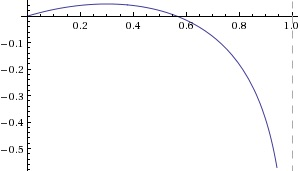
\includegraphics[width=\linewidth]{plotGF}}
      \caption{La función $g(f)$ siempre encuentra un máximo y después tiende a $-\infty$}\label{Fig:Gf}
    \end{minipage}
 \end{figure}
 
 A continuación se presenta un teorema que enumera las ventajas de maximizar $g(f)$, dentro de estas pautas se presentan propiedades básicas que cumplen el criterio de Kelly y dan a entender mejor su función en cada apuesta. La prueba de este teorema se omite en esta tesis, pero se puede revisar en Thorp\cite{thorp1969optimal} para el caso de una simple binomial y para un caso más general se deber revisar Breiman\cite{breiman1961optimal}.
 
\begin{itshape}

\paragraph{Teorema} % (fold)
\label{par:teorema}

\begin{enumerate}

	\item Si $g(f) > 0$, entonces $\lim_{n\to\infty}X_n = \infty$ casi seguro. Es decir, para cada $M$ se tiene que $p(\lim \inf{n\to\infty}X_n >M)=1$.

	\item Si $g(f) < 0$, entonces $\lim_{n\to\infty}X_n = 0$ casi seguro. Es decir, para cada $\varepsilon > 0 $ se tiene que $p(\lim \sup_{n\to\infty}X_n <\varepsilon)=1$.
	
	\item Si $g(f) = 0$, entonces $\lim \sup_{n\to\infty}X_n = \infty$ casi seguro y $\lim \inf_{n\to\infty}X_n = 0$ casi seguro.

	\item Dada una estrategia $\phi^*$ que maximiza $E(\log(X_n))$ y cualquier otra estrategia $\phi$ ``esencialmente diferente'' (No necesariamente una estrategia de apuestas fraccionada fija), entonces $\lim_{n\to\infty}X_n(\phi^*)/X_n(\phi)=\infty$ casi seguro.

	\item El tiempo esperado para que la cantidad de capital actual $X_n$ alcance alguna meta fija $C$ es asintóticamente menor con una estrategia que maximice $E(\log(X_n))$.

	\item Supóngase que el retorno en una unidad apostada en el i-ésimo ensayo es la variable aleatoria $U_i$, además supóngase que la probabilidad de éxito es $p_i$ donde $1/2 < p_i < 1$. Entonces, $E(\log(X_n))$ se maximiza escogiendo en cada ensayo la fracción $f_i^* = p_i -q_i$ que maximiza $E(\log(1+f_iU_i))$.

\end{enumerate}
% paragraph Teorema 1 (end)
\end{itshape}

De la parte 1 de este teorema se muestra que excepto para un número finito de términos, el capital del jugador $X_n$ sobrepasará una cota fija $M$ cuando $f$ se escoge dentro del intervalo $(0,f_c)$. Pero, si $f>f_c$, entonces la parte 2 muestra que la ruina será casi segura. La parte 3 demuestra que si $f=f_c$, entonces $X_n$ (casi seguro) oscilará aleatoriamente entre $0$ y $\infty$. Las partes 4 y 5 establecen que la estrategia de Kelly de maximizar $E(\log(X_n))$ es asintóticamente óptima ya que si se toma una estrategia ``esencialmente diferente'' como aquella tal que la diferencia, $E(\log(X_n^*)) - E(\log(X_n))$, entre la estrategia de Kelly y cualquier otra estrategia crece más rápido que la desviación estándar de $\log(X_n^*) - \log(X_n)$, asegurando $p(\log(X_n^*)-\log(X_n)>0) \to 1$. Finalmente, la parte 6 establece la validez de utilizar el método de Kelly para escoger $f_i*$ en cada uno de los ensayos (aun cuando las probabilidades cambian de un ensayo a otro) con el fin de maximizar $E(\log(X_n))$.

\subsubsection{Ejemplificando Kelly} % (fold)
Retómese la situación descrita al principio de esta sección de un jugador contra un adversario infinitamente rico. Supóngase que el jugador gana la apuesta con una probabilidad $p=0.53$, que su capital inicial es de $X_0$ y que su capital es infinitamente divisible y disponible para apostar. Aplicando el Teorema parte 5, se tiene que $f^* = p-q =0.53-0.47 = 0.06$. Es decir, el jugador debe apostar $6\%$ de su capital para hacerlo crecer $X_n$ a la mayor tasa posible con probabilidad cero de irse a la quiebra. De igual manera, si el jugador continuamente apuesta una fracción más pequeña que el $6\%$, también su capital se irá al infinito, pero la velocidad de crecimiento será menor.

Ahora, si se resuelve numéricamente la ecuación $g(f) = 0.53\log(1+f)+0.47\log(1-f)=0$ se obtiene que $f_c= 0.119712...$. Esto quiere decir que el usuario puede apostar hasta tantito menos del $12\%$ de su capital y como en el caso anterior, su capital se iría al infinito pero a menor escala que con el óptimo. Después del $12\%$, aunque el jugador pudiera ganar dinero a una velocidad mayor que la de la estrategia óptima, al final su capital se irá a cero (casi seguro). 

En cuanto a la tasa de crecimiento, se tienen que $g(f*)= 0.001801$ por lo que después de $n$ apuestas exitosas, su capital crecerá $0.001801n$ veces más dinero que con el que comenzó. De aquí se puede calcular el tiempo esperado de doblar la cantidad de dinero del capital, se tiene que $0.001801n=\log2$. Es decir que después de $n=385$ ensayos se estará doblando la cuenta del jugador.
% paragraph ejemplificando (end)

\subsubsection{Aplicando Kelly a las apuestas de futbol} % (fold)
\label{subsubsection:aplicando_kelly_a_las_apuestas_de_futbol}

El criterio de Kelly se puede extender a las apuestas de futbol. Retómese la situación original, pero ahora considerando que el jugador puede ganar $b$ pesos por cada peso invertido en la apuesta. Además, considérese que el jugador seleccionará sólo apuestas favorables, es decir que sólo apostará cuando la probabilidad de ganar $p>0$ sea ventajosa, i.e. $pb - q > 0$.
De la misma manera se maximiza la siguiente función\footnote{Esta optimización y la fórmula, que a la fecha es tan usada por todos los sitios de apuestas, tuvo su aparición en  Thorp \cite{thorp1969optimal}, aquí mismo se puede encontrar su demostración formal}:
\[g(f) = E\left(log(\frac{X_n}{X_0})\right)=p\log(1+bf)+q\log(1-f)\]
Y se obtiene que:
\[f^* = \frac{bp -q}{b}\]
Esta $f^*$ dicta la fracción del capital que el jugador debe apostar en \textbf{cada} apuesta. Es decir, que la cantidad a apostar depende de dos cosas: Primero, de la probabilidad de éxito de la apuesta. Segundo, del posible retorno de inversión de la apuesta (momio).

\subsubsection{Ejemplo. Kelly en apuestas de futbol}

\emph{Tómese el siguiente partido, Real Madrid vs Juventus. El análisis que se realizó del partido sugiere que la probabilidad de ganar de la Juventus es de $54\%$. Curiosamente, el momio de esta apuesta es $6.75$
¿Cuál es la cantidad de dinero que se debe jugar en esta favorable apuesta?}\linebreak[2]


La solución viene de evaluar $f^*$:
\[f^* = \frac{bp -q}{b} = \frac{(6.75-1)*0.54 - 0.46}{6.75-1} = 0.46\]
Por lo tanto, en este inimaginable escenario, se debe jugar el $46\%$ del capital total en esta apuesta.
\linebreak[2]



Hay tres quejas a considerar sobre Kelly: La primera tiene que ver con el supuesto de ``divisibilidad infinita'', ya que las casas de apuestas usualmente tienen una cantidad mínima para las apuestas y algunas casas tienen todas sus apuestas en función de múltiplos de estos mínimos (o créditos), esto implica que  (casi seguro) siempre se alcanza la ruina. La segunda, va más enfocada a los mercados financieros que implican la posibilidad de pérdidas (``commodity futures'' o ``securities short sales''), en estos casos se puede perder una cierta cantidad de dinero $a$ con probabilidad $q$. Entonces, al resolver, se tiene que la esperanza es igual a $m=bp-aq>0$, $f^*=m/ab >0$; para este caso, se sugiere al lector revisar Thorp y Kassouf \cite{thorp1967beat} y revisar en su detalle la generalización de la formulación y sus detalles. Finalmente, como se vio en los tiempos esperados para duplicar el capital, Kelly es muy lento en el crecimiento del capital al garantizar la ruina con probabilidad $0$; esto hace que en temporadas de futbol (con una cantidad de juegos) el criterio sirva únicamente de guía.

Browne \cite{browne2000can} llama al criterio de Kelly \cite{kelly1956new} como la estrategia óptima de crecimiento, o como la estrategia de utilidad logarítmica. Menciona que es óptima cuando en una variedad de circunstancias la ganancia crece multiplicativamente, únicamente. Hace énfasis que la mayoría de las propiedades de optimalidad son asintóticas en naturaleza (hacia un horizonte infinito), en su trabajo analiza las propiedades de la estrategia de Kelly a corto plazo.


 \section{Proceso para la selección de apuestas}

% Uno de los conceptos más imporantes en la teoría de probabilidad es el del valor esperado de una variable aleatoria\footnote{Retómese el concepto de variable aleatoria más usual, se puede utilizar la definición del capítulo 4 del libro de Ross \cite{ross2006first}, una función $X$ que genera valores aleatorios reales en un espacio muestral completamente definido.}, en palabras del señor Ross \cite{ross2006first} el valor esperado de $X$ se define como un promedio ponderado de los valores posibles que puede tomar $X$; se pondera cada valor con la probabilidad de que $X$ tome ese preciso valor.
%  \begin{itemize}
%
%  	\item Valor esperado de una variable discreta.
%
% 		\[E[X] = \sum_{x:p(x)>0}x p(x)\]
%  	\item Valor esperado de una variable continua.
% 	\[E[X] = \int_{-\infty}^{infty} f(x) dx\]	
 % \end{itemize}
 
 El proceso de la recomendación de apuestas se puede dividir en cinco pasos principales:

 \begin{enumerate}
 	\item \textbf{Determinación de apuestas redituables.} De todas las apuestas de las cinco ligas que haya en la jornada a recomendar, se escogen únicamente aquellas que sean redituables a largo plazo. Independientemente del nivel de riesgo de cada cliente, se generarán recomendaciones únicamente de apuestas que, al analizarlas, tengan ganancias esperadas.
 	\item \textbf{Selección de apuestas de acuerdo al riesgo del cliente.} Las estimaciones de cada partido tienen un intervalo de confianza. Con base en este intervalo y el perfil de riesgo del usuario se seleccionan las apuestas.
 	\item \textbf{Cálculo de la proporción del dinero a invertir por apuesta.} Al conocer la selección de las apuestas, se calcula la proporción de dinero a invertir para cada apuesta, este proceso sigue siendo dependiente de la confianza de la estimación del partido y de la aversión al riesgo del cliente.
 	\item \textbf{Determinación del nivel de reservas.} En este paso se cuenta con un conjunto seleccionado de apuestas y la proporción de dinero que se debe invertir para cada una de ellas. Acorde a su encuesta, se calcula el nivel óptimo de reservas que le permitan al cliente seguir apostando a pesar de que tenga una mala jornada y pierda todas las apuestas.
 	\item \textbf{Recomendación.} Todos estos elementos constituyen en su totalidad la recomendación de la semana que se presenta en el portal al cliente.
 \end{enumerate}
 
Para definir el escenario completo es necesario definir las variables que se utilizan en el proceso, así como las funciones de utilidad que modelan los perfiles de riesgo de los usuarios. Después de estas dos sub-secciones se retomará paso a paso la explicación del proceso de recomendación de apuestas.
 
\subsection{Variables necesarias}
\label{subsec:variables-necesarias}
En este apartado de la tesis se explica cómo se determinan los partidos que se recomiendan a los clientes.
Las variables que se necesitan utilizar son las siguientes:
\begin{enumerate}
	\item \textbf{Probabilidades.} Ya en apartados anteriores se habló de las probabilidades estimadas de que ocurran los tres diferentes resultados de cada encuentro de la jornada (Victoria del local, del visitante y empate). Estas probabilidades son alimentadas a través del portal administrativo.
	
	\item \textbf{Momios.} Los momios que generan las casas de apuestas para cada partido. En la mayoría de los escenarios el usuario escoge usar todos los momios de todos los bookies, en estos casos se tomarán los momios que ofrezcan mejores retornos para cada partido. Estos momios se toman de la información pública de las casas de apuestas.
	
	\item \textbf{Variables de riesgo.} Se tienen tres elementos principales que generan la noción de riesgo en el sistema:
	\begin{itemize}
		\item \textbf{Función de utilidad en selección.} Determina los partidos redituables de la jornada.
		\item \textbf{Función de utilidad del dinero.} Dicta la proporción de dinero a apostar en cada partido.
		\item \textbf{Variable de reserva.} Marca la cantidad de dinero que el cliente debería guardar para siguientes apuestas.
		Estas variables dependen de la encuesta que se le presenta al cliente al crear su cuenta.
	\end{itemize}
	
	\item \textbf{Variable de evolución de ingreso del cliente.} Se define como la cantidad de dinero que tiene el cliente en esta jornada entre la máxima cantidad de dinero que ha tenido. Esta variable genera una noción, en caso de que existan, de la magnitud de las pérdidas que ha tenido el cliente.
\end{enumerate}

\subsection{Funciones de utilidad}
Para modelar el comportamiento de un individuo ante el riesgo, se utilizan funciones de utilidad. Estas funciones representan la utilidad (o beneficio) que un individuo puede obtener por una apuesta. Las funciones más arriesgadas le dan valores mayores valores a las apuestas que que ofrecen las mejores ganancias y las funciones más conservadoras favorecen aquellas apuestas con mayores probabilidades.
En particular, se podría decir de manera intuitiva que el valor obtenido por una función de utilidad para una apuesta en particular es la cantidad de unidades de dinero que el individuo estaría dispuesto a invertir en esa apuesta.
El siguiente listado presenta las funciones que se utilizan actualmente en el sistema.
\begin{enumerate}
		\item \textbf{Polinomial - lineal:} 
		\[f_1(\alpha, p, m) = \left(\frac{p}{1-p} \right)^\frac{1}{1-\alpha}(m-1)^\frac{\alpha}{1-\alpha}\]
Parámetro $\alpha$ que va de cero a uno. Es una de las familias más volátiles en cuanto al riesgo, para valores cercanos a uno del parámetro tiende a ser muy arriesgada, casi sin diversificar, y para valores cercanos a cero tiende a ser muy conservadora y suele diversificar mucho más en las apuestas.

		\item \textbf{Polinomial - cuadrática:} 
		\[f_2(\alpha, p, m) = \left(\frac{p}{1-p} \right)^\frac{1}{2-\alpha}(m-1)^\frac{\alpha}{2-\alpha}\]
Esta familia de funciones es muy parecida a la anterior, también tiene un parámetro $\alpha$ entre cero y uno, sólo que en este caso no es tan extremista como en el caso anterior.
		
		\item \textbf{Exponencial - lineal:} 
		\[f_3(\alpha, p, m) = \left(\frac{1}{m-1} \right)ln\left(\frac{\alpha p(m-1)}{1-p}\right)\]
Esta familia de funciones tiene un parámetro $\alpha$ que es mayor a uno. Es una familia de funciones conservadoras que suelen proteger muy bien adelantándose a semanas malas, a costo que en semanas buenas no logran tan buenos beneficios.
		
		\item \textbf{Lineal - exponencial:} 
		\[f_4(\alpha, p, m) = ln\left(\frac{p(m-1)}{1-p}\right) + ln(\alpha)\]
Esta familia de funciones tiene un parámetro $\alpha$ que es mayor a uno. Es una familia de funciones que le gusta fuertemente diversificar, aparte tiende a favorecer un poco aquellas apuestas más riesgosas.

		\item \textbf{Logarítmica - polinomial:} 
		\[f_5(\alpha, p) = \left(\frac{p}{1-p}\right)^\frac{1}{\alpha}\]
Parámetro $\alpha$ mayor a uno. Es una familia de funciones muy conservadora ya que toma valores sin considerar los momios del mercado, al tomar en cuenta solamente las probabilidades de los partidos tiende a ser más estable en el tiempo.

		\item \textbf{Tangente - lineal:} 
		\[f_6(\alpha, p, m) = \frac{1}{m-1}\sqrt{\frac{pm - (1-\alpha)p - \alpha}{1-p}}\]
		Parámetro $\alpha$ entre cero y uno. Esta familia es la más conservadora de la lista, busca tener las menores pérdidas posibles y protege las inversiones cada semana.
\end{enumerate}

Estas seis funciones son las que utiliza Egobets para modelar la aversión al riesgo de sus clientes. Cuando ellos llenan la encuesta del perfil, realmente están seleccionando una de estas funciones.


\subsection{Paso 1 - Determinación de apuestas redituables}
\label{sec:paso-1}


Para seguir la explicación de los pasos del proceso se tomará un ejemplo práctico y las transformaciones que sufre durante el proceso. Al empezar las recomendaciones de una jornada se tiene un conjunto de datos muy parecido al que se da en el ejemplo. Tómese la tabla~\ref{momios-y-probas} como base del ejemplo. En esta tabla se presentan momios de alguna casa de apuesta (usualmente los mejores del mercado) para diez partidos distintos, cada uno cuenta con los momios para los tres tipos de apuestas: victoria del Local ($m_L$), empate ($m_E$) y victoria del visitante ($m_V$). Además se muestran las probabilidades estimadas por Egobets de los tres posibles resultados del encuentro: victoria del local ($\hat{p_L}$), empate ($\hat{p_L}$) y victoria del visitante ($\hat{p_L}$).

\begin{table}[ht]
\centering
\resizebox{\textwidth}{!}{%
\begin{tabular}{|c|ccc|ccc|}
\toprule
{\textbf{Partido}}                 & $\mathbf{m_L}$ & $\mathbf{m_E}$ & $\mathbf{m_V}$ & $\mathbf{\hat{p_L}}$ & $\mathbf{\hat{p_E}}$ & $\mathbf{\hat{p_V}}$ \\ \midrule
A & 2.6  & 3.2  & 2.75  & 0.31  & 0.23  & 0.46  \\ 
B & 2.1  & 3.3  & 3.5   & 0.37  & 0.3   & 0.32  \\ 
C & 1.11 & 8.5  & 21    & 0.84  & 0.1   & 0.04  \\ 
D & 4.5  & 3.75 & 1.72  & 0.29  & 0.27  & 0.45  \\ 
E & 2    & 3.4  & 3.75  & 0.37  & 0.31  & 0.31  \\ 
F & 1.53 & 4    & 6     & 0.61  & 0.17  & 0.21  \\ 
G & 2.1  & 3.25 & 3.6   & 0.51  & 0.24  & 0.25  \\ 
H & 1.9  & 3.4  & 4     & 0.42  & 0.29  & 0.29  \\ 
I & 1.8  & 3.5  & 4.5   & 0.46  & 0.29  & 0.25  \\ 
J & 1.9  & 3.4  & 4     & 0.5   & 0.26  & 0.23  \\ \bottomrule
\end{tabular}
}
\caption{Diez partidos con sus respectivos momios y las probabilidades estimadas por Egobets}
\label{momios-y-probas}
\end{table}

Para concretar el ejemplo, se fijarán las siguientes funciones y variables.
\begin{itemize}
	\item \textbf{Función de selección.} Tómese la \emph{Polinomial - lineal} $f_1$ con parámetro $\alpha = 0.4$.
	\item \textbf{Función de utilidad del dinero.} Úsese la \emph{Exponencial - lineal} con parámetro $\alpha = 3$
	\item \textbf{Variable de reserva.} Será $v_R = 15$.
	\item \textbf{Variable de ingreso.} Será $v_I = 0.80$.
\end{itemize}
	

Ahora para proceder al primer paso, defínase el valor esperado de una apuesta como la multiplicación de la probabilidad de que suceda el resultado por el momio que se tiene para esa apuesta. 
Con el ejemplo bien definido se procede a filtrar las apuestas con el primer paso. De manera intuitiva, se podría enunciar que el valor esperado de una apuesta corresponde a la cantidad de unidades de dinero que se obtienen por cada unidad de dinero invertida\footnote{Recuérdese que esta cantidad incluye la cantidad de dinero invertida en la apuesta. También recuérdese que la ganancia solamente se obtiene si se gana la apuesta.}

Entonces, el primer paso consiste en utilizar para las recomendaciones, sólo las apuestas con ganancias a largo plazo; las otras apuestas tendrán un valor esperado no positivo, es decir, no garantizan más que pérdidas a largo plazo. Más aun, se usarán solo las apuestas que garanticen un valor esperado mayor a $1.025$, esta restricción tiene dos ventajas, la primera es que las probabilidades que se usan son estimaciones por lo que ese $2.5\%$ funciona como protección para no caer en valores esperados negativos y la segunda es que si el rendimiento es tan pequeño toma mucho tiempo para un cliente ir acumulando ganancias. 

\begin{table}[ht]
\centering
\resizebox{\textwidth}{!}{%
\begin{tabular}{|c|ccc|ccc|ccc|c|}
\toprule
Partido & $\mathbf{m_L}$ & $\mathbf{m_E}$ & $\mathbf{m_V}$ & $\mathbf{\hat{p_L}}$ & $\mathbf{\hat{p_E}}$ & $\mathbf{\hat{p_V}}$ & $\mathbf{m_L\cdot\hat{p_V}}$ & $\mathbf{m_E\cdot\hat{p_E}}$ & $\mathbf{m_V\cdot\hat{p_V}}$ & \textbf{Apuesta} \\ \midrule
A & 2.6 & 3.2 & 2.75 & 0.31 & 0.23 & 0.46 & 0.81 & 0.74 & \textbf{1.27} & Visitante \\
B & 2.1 & 3.3 & 3.5 & 0.37 & 0.3 & 0.32 & 0.78 & 0.99 & \textbf{1.12} & Visitante \\
C & 1.11 & 8.5 & 21 & 0.84 & 0.1 & 0.04 & 0.93 & 0.85 & 0.84 & Ninguna \\
D & 4.5 & 3.75 & 1.72 & 0.29 & 0.27 & 0.45 & \textbf{1.31} & 1.01 & 0.77 & Local \\
E & 2 & 3.4 & 3.75 & 0.37 & 0.31 & 0.31 & 0.74 & \textbf{1.05} & \textbf{1.16} & Empate/Visitante \\
F & 1.53 & 4 & 6 & 0.61 & 0.17 & 0.21 & 0.93 & 0.68 & \textbf{1.26} & Visitante \\
G & 2.1 & 3.25 & 3.6 & 0.51 & 0.24 & 0.25 & \textbf{1.07} & 0.78 & 0.90 & Local \\
H & 1.9 & 3.4 & 4 & 0.42 & 0.29 & 0.29 & 0.80 & 0.99 & \textbf{1.16} & Visitante \\
I & 1.8 & 3.5 & 4.5 & 0.46 & 0.29 & 0.25 & 0.83 & 1.02 & \textbf{1.13} & Visitante \\
J & 1.9 & 3.4 & 4 & 0.5 & 0.26 & 0.23 & 0.95 & 0.88 & 0.92 & Ninguna\\ \bottomrule
\end{tabular}
}
\caption{Escogiendo apuestas que vale la pena realizar}
\label{redituables}
\end{table}

Obsérvese en la tabla~\ref{redituables} como en negritas se han señalado las posibles apuestas a realizar. De las treinta posibles apuestas, ahora sólo quedan 9 redituables. Hay dos partidos el `C' y el `J' que no ameritan apuesta alguna. Y el partido `E', por ejemplo, tiene dos posibles apuestas redituables.

\subsection{Paso 2 - Selección de apuestas}
\label{sec:paso-2}


Para determinar el portafolio de apuestas basta con calcular el valor de la función de utilidad de selección y se deben tomar aquellas ``$n$'' apuestas que tengan los mayores valores (Donde ``$n$'' es el número de apuestas a recomendar).
Ver tabla~\ref{seleccion}

\begin{table}[ht]
\centering
\resizebox{\textwidth}{!}{%
\begin{tabular}{|c|c|c|c|c|}
\toprule
\textbf{Partido} & \textbf{Apuesta} & \textbf{Momio} & $\mathbf{\hat{p}}$ & $\mathbf{f_1(\alpha, p, m)}$ \\ \midrule
A & Visitante & 2.75 & 0.46 & \textbf{1.07} \\
B & Visitante & 3.5 & 0.32 & 0.53 \\
D & Local & 4.5 & 0.29 & 0.49 \\
E & Empate & 3.4 & 0.31 & 0.48 \\
E & Visitante & 3.75 & 0.31 & 0.53 \\
F & Visitante & 6 & 0.21 & 0.31 \\
G & Local & 2.1 & 0.51 & \textbf{1.12} \\
H & Visitante & 4 & 0.29 & 0.48 \\
I & Visitante & 4.5 & 0.25 & 0.36\\ \bottomrule
\end{tabular}
}
\caption{Escogiendo apuestas que vale la pena realizar}
\label{seleccion}
\end{table}

\subsection{Paso 3 - Calcular cuanto dinero a cada apuesta}
\label{sec:paso-3}

Una vez determinado el portafolio de apuestas hace falta determinar la cantidad de dinero que se invertirá en éste. Esta sección y la próxima resolverán tal problema.
 Se empieza por determinar cuál es la proporción de dinero que se invertirá en cada apuesta. La solución es sencilla, ya se determinó en secciones anteriores que el valor definido por una función de utilidad puede ser comparado con la cantidad de unidades de dinero que una persona estaría dispuesta a invertir en una apuesta en particular. El único problema con este enfoque es que tales cantidades no se encuentran en ninguna escala (es decir, dólares, pesos, etc).Se hace lo siguiente: para cada apuesta se calcula el valor de su función de utilidad del dinero y después lo dividimos entre la suma de todos estos valores para todas las apuestas que se van a tomar, de esta forma se tiene los números como porcentajes.
 Regresando al ejemplo: (En este caso la función de utilidad del dinero era Exponencial-Lineal con parámetro 3)
Ver tabla~\ref{proporcion}

\begin{table}[ht]
\centering
\resizebox{\textwidth}{!}{%
\begin{tabular}{|c|c|c|c|c|}
\toprule
\textbf{Partido} & \textbf{Apuesta} & \textbf{Momio} & $\mathbf{\hat{p}}$ & $\mathbf{f_3(\alpha, p, m)}$ \\ \midrule
A & Visitante & 2.75 & 0.46 & 0.23 \\
G & Local & 2.1 & 0.51 & 0.35 \\ \bottomrule
\end{tabular}
}
\caption{Calculando la proporción del dinero que se debe invertir en estas apuestas}
\label{proporcion}
\end{table}


Los valores suman a 0.59, cuando se divide cada valor por 0.59 resulta: De la cantidad a apostar, se debe de apostar $40 \%$ en el partido A a visitante y $60 \%$ en el partido G a local.


\subsection{Paso 4 - Determinar nivel de reservas}
\label{sec:paso-4}

%[COMENTARIO]ESto no creo que vaya aquí, estas propiedades deberían estar definidas en otro lugar
% El sistema de reservas, en pocas palabras, tiene como intención proteger el dinero de los clientes en el corto plazo, de tal forma que si una semana resulta en pérdidas, éstas no vayan a afectar la tendencia a largo plazo de sus ingresos totales. Las ventajas de usar un sistema de reservas son las siguientes: primero, como ya se dijo, proteger el dinero del cliente en el corto plazo cuando haya pérdidas, en segundo lugar, permite al cliente mantener el mismo nivel de apuestas cada semana, y tercero, permite darle una estructura de fondo de inversión a las apuestas y así poder aprovechar el potencial interés compuesto que resulte de apostar. En contraste, las desventajas son: en cada semana se decide apostar menos dinero y por lo tanto las ganancias son menores en el corto plazo, además al ser una estrategia de largo plazo, los clientes que deseén incurrir en mayores riesgos no usarán este sistema de reservas.
%
% Un sistema de reservas da más flexibilidad de la que inicialmente se podría pensar, estas son algunas de las propiedades que serían deseables en un sistema de esta forma:
% \begin{enumerate}
% \item Se tenga la seguridad de que con alta probabilidad el apostador nunca va a perder todo su dinero.
%
% \item Que en aquellas semanas que son mas riesgosas se apueste menos dinero, para protegerse del riesgo.
%
% \item Que en aquellas semanas donde se pueden tener muchas ganancias se apueste una mayor cantidad de dinero, para tratar de aprovechar situaciones ventajosas.
%
% \item Que cuando se tengan pérdidas se apueste una mayor cantidad de dinero para tratar de recuperar el nivel anterior de ganancias lo más pronto posible.
% \end{enumerate}
% Como se ve, este sistema tiene la propiedad de ser dinámico y que depende tanto de las circunstancias de las apuestas como también del historial de ganancias del cliente.

Determinar el nivel de reservas es un algoritmo que depende del historial de ganancias del cliente así como de las circunstancias de las apuestas que se le presentan al cliente. A continuación se explica paso a paso como determinar el nivel de reservas.

\begin{enumerate}
	\item \textbf{Calcular la cantidad de partidos a los que se apuesta.}
	
	
Defínase $j$,$k$ como la cantidad de partidos a apostar y el número de apuestas a tomar, respectivamente.
En este pasó bastará con calcular $j$. Sin embargo, es importante notar que hay veces en las que puede haber más de una apuesta sugerida para un mismo partido, i.e. $k>j$. En estos casos se deberá ser cuidadoso de no contar doble los partidos que ya tengan apuestas.

	% Sea $k$ el número de a
	% \lstset{language=Pascal}
	% \begin{lstlisting}[frame=single]
	% begin
	% 	apuestas := 0;
	% 	aux2 := 0;
	% 	for i:= 1 to K do
	% 	begin
	% 		if (proporcion(i) >= 1/k) then
	% 			aux1 := aux1 + 1;
	% 		else
	% 			aux2 := aux2 + proporcion(i);
	% 	end;
	% 	partidosApostables := aux1 + round((k)aux2);
	% end.
	% \end{lstlisting}
	%
	\item \textbf{Calcular el valor esperado y varianza del portafolio de apuesta.}
	
	
	Sean $m_i$, $p_i$ y $prop_i$; el momio, la probabilidad y la proporción de dinero a apostar del partido $i$ respectivamente. Entonces el valor esperado de la apuesta sería:
	\[\mu = \sum_{i=1}^{k}{(prop_i)(m_i)(p_i)}\]
	Y el riesgo o varianza del portafolio de apuestas se calcula así:
	\[\sigma = \sqrt{\sum_{i=1}^{k}{(prop_i))^2(m_i)^2(p_i)(1-p_i)}}\]
	
	
	\item \textbf{Actualizar el riesgo del portafolio.}
	
	
	Sea $\rho$ el parámetro de reserva un número entero entre $10$ y $25$ dependiendo de la encuesta del cliente. Se actualiza el riesgo del portafolio al multiplicarlo por un escalar proveniente de la raíz cuadrada del cociente de la cantidad de partidos $j$ entre el parámetro de reserva $\rho$.
	\[\sigma = \left(\sqrt{\frac{j}{\rho}}\right)\sigma\]
	

	\item \textbf{Calcular probabilidad de riesgo.}
	
	Sea $X$ la variable de evolución del ingreso del cliente (Esta variable es completamente dependiente de las historia de perdidas y ganancias del cliente). Y sea $p_\sigma$ la probabilidad de riesgo y se calcula de la siguiente manera:
	\[p_\sigma = \frac{1}{1.749615}(I_1 + I_2) - 1.06 + X\]
	Donde $I_1$ es
	\[I_1 = 0.2925 +1.3772\mu - 1.127\rho\]
	e $I_2$ equivale a
	\[I_2 = \frac{3.11}{\mu}(1 + 0.792\sigma - \mu)((-0.567345 + 1.3772\mu -1.17\sigma)\mu X)^{0.123}\]
	
	
	\item \textbf{Calcular variable proxy.}
	
	 Sea $proxy$ la variable auxiliar que tome en cuenta la probabilidad de riesgo en el cálculo.
	 \[proxy = 0.2925 + 1.3772\mu -1.127\sigma - 0.9975p_\sigma\]
	
	\item \textbf{Calcular el nivel de reserva.}
	
	Finalmente, defínase $c_A$ cómo el porcentaje a apostar del ingreso total. El nivel de reserva será uno menos esta proporción.
	
	\begin{equation*}
	    c_A = \begin{cases}
	               0.05            & \text{si } \frac{j(proxy)}{\rho} < 0.05\\
	               1               & \text{si } \frac{j(proxy)}{\rho} >1\\
	              	\frac{j(proxy)}{\rho} & \text{en otro caso}
	           \end{cases}
	\end{equation*}
	
	$C_A$ representa, en porcentaje, la cantidad de dinero que se le recomendará al cliente que apueste en esa semana para el portafolio de apuestas en cuestión.
	
	\textbf{Calculando el nivel de reserva en el ejemplo.}
	
	Primero que nada es importante recordar cuanto valían las distintas variables y establecer los valores necesarios para el ejemplo.
	\begin{itemize}
		\item $k = 2$ (Cantidad apuestas a realizar)
		\item $\rho = 15$ (Parámetro de reserva en función de las preferencias del cliente)
		\item $X = 0.80$ (Evolución del ingreso del cliente)		
	\end{itemize}
	Ahora se procederá a calcular el nivel de reservas.
	\begin{enumerate}
		\item Se obtiene $j = 2$ (Cantidad de partidos en los que se apuesta)
		\item Se calcula el valor esperado 
		\[\mu = (0.4)(2.75)(0.46) + (0.6)(2.1)(0.51) = 1.1486\] 
		y el riesgo del portafolio 
		\[\sigma = \sqrt{(0.4)^2(2.75)^2(0.46)(0.54)+(0.6)^2(2.1)^2(0.51)(0.49)} = 0.835\]
		\item Se actualiza el riesgo $\sigma = \left(\sqrt{\frac{2}{15}}\right)0.835 = 0.3$
		\item Se calcula la probabilidad de riesgo
		\[I_1 = 0.2925 +1.3772(1.1486) - 1.127(0.3) = 1.53\]
		\[I_2 = \frac{3.11}{1.1486}(1 + 0.792(0.3) - \mu)((-0.567345 + 1.3772(1.1486)\]
		\[-1.17(0.3))(1.1486)(0.8))^{0.123} = 0.2272\]
		Entonces
		\[p_\sigma = \frac{1}{1.749615}(1.53 + 0.2272) - 1.06 + 0.8 = 0.74\]
		
		\item Se calcula la variable auxiliar $proxy = 0.2925 + 1.3772(1.1486) -1.127(0.3) - 0.9975(0.74) = 0.81$
		
		\item La cantidad a apostar es entonces es igual a $c_A = \frac{2(0.81)}{15} = 0.108$
		Por lo tanto, con esta aversión al riesgo y con base en el portafolio de apuestas de la tabla~\ref{proporcion}.
		
		\textbf{El nivel de reserva para esta recomendación es del} $\mathbf{89.2\%}$.
	\end{enumerate}
\end{enumerate}

\subsection{Paso 5 - Presentando la recomendación}
\label{sec:paso-5}
Ahora, con todos los pasos cumplidos lo único restante es poner las cifras juntas. Se toma la proporción calculada en~\ref{sec:paso-3} y se multiplica por la cantidad a apostar obtenida en~\ref{sec:paso-4}.
Más aún, si el usuario proporciona la cantidad de dinero que tiene disponible, las recomendaciones se pueden expresar en moneda.

Finalmente si para el ejemplo planteado en~\ref{sec:paso-1} se conoce que el usuario tiene $\$10'000.00$ para apostar, la recomendación de apuesta quedaría de la siguiente manera:
\begin{enumerate}
	\item Apueste $\$432$ pesos ($4.32\%$) en el partido A a favor del equipo visitante.
	\item Apueste $\$648$ pesos ($8.48\%$) en el partido G a favor del equipo local.
\end{enumerate}


 %Egobets
\chapter{Plataforma de recomendaciones}
\label{chap:software}
\graphicspath{{/Users/brunomedina/Dropbox/Tesis-Egobets/egobets-notas/resources/diagramas/}}

Egobets.com proporciona al cliente los servicios de asesoría de apuestas personalizada a través de un portal Web usable, práctico y profesional. En este capítulo se presenta el sistema desarrollado con los fundamentos teóricos descritos en los capítulos anteriores, una verdadera aplicación computacional de las matemáticas

% Se describen las cuatro piezas de software desarrolladas que conforman en su totalidad el sistema de Egobets. Las tres primeras permiten al usuario adminstrativo echar a andar toda la maquinaria. Y la última pieza, conocida como e
% A todo este conjunto de herramientas y programas que el usuario necesita para esta tarea se le conocerá como \emph{Back Office}.




\section{Diseño y arquitectura}
\label{sec:design}
Egobets.com es un sistema con arquitectura cliente-servidor montado sobre una máquina virtual con sistema operativo Ubuntu Linux en la nube de ``Amazon Web Services (AWS)''. En esta sección se presentan los diagramas que describen la arquitectura del sistema, se muestran las ventajas de utilizar el cómputo en la nube, se presentan las tecnologías más relevantes involucradas en el sistema y también se expone el patrón de diseño \textit{Modelo Vista Controlador} junto con su respectiva representación gráfica de base de datos.
\subsection{Ventajas de correr Egobets en la nube}
\begin{figure}[!htb]\centering
   \begin {minipage}{1\textwidth}
     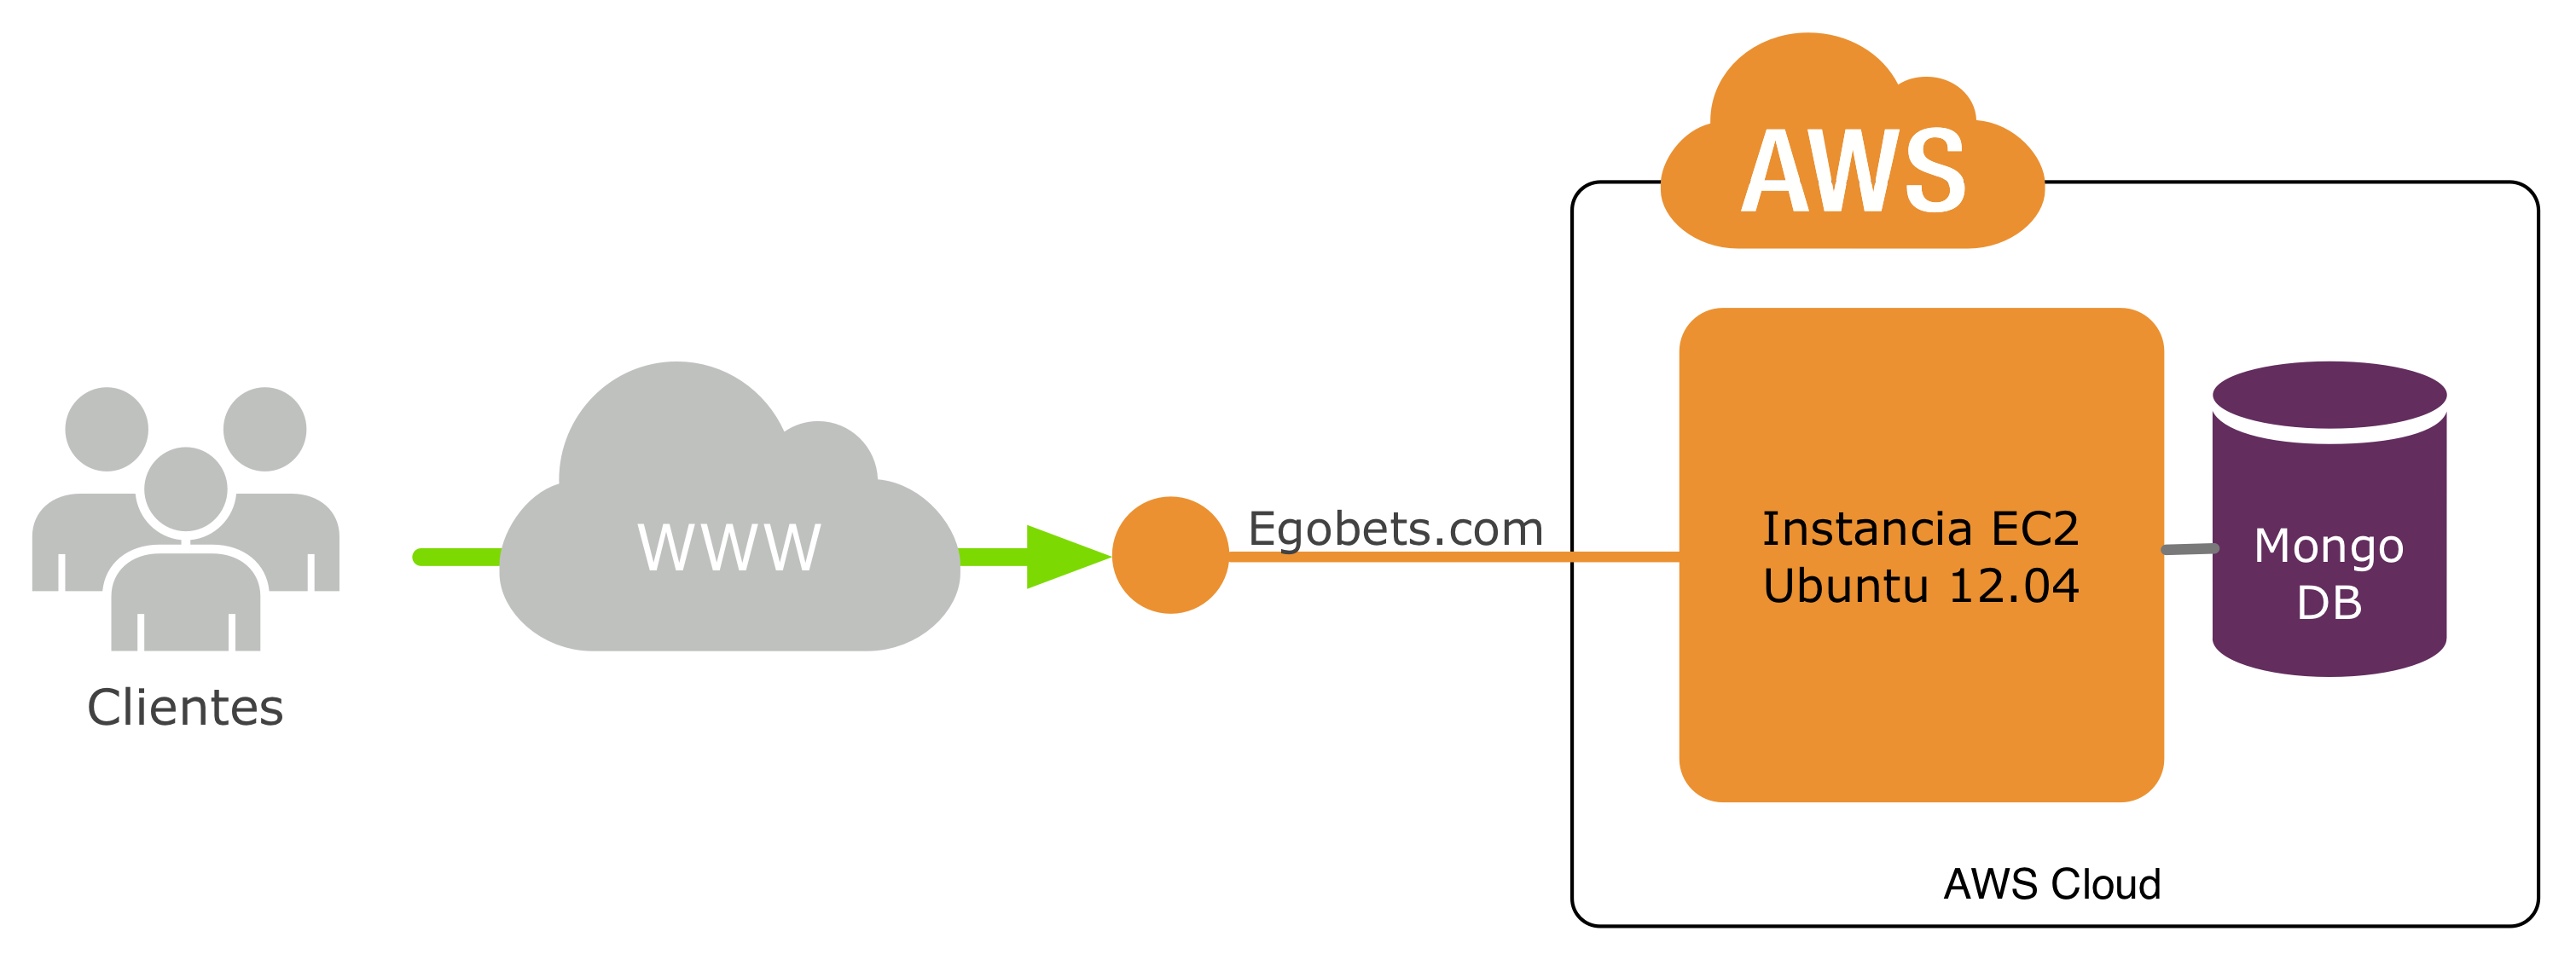
\includegraphics[width=\linewidth]{diagrama-portal-publico}
     \caption{Arquitectura Cliente Servidor sobre Nube de AWS}\label{Fig:diagrama-portal-publico}
   \end{minipage}
\end{figure}

El sistema usa la nube de AWS para ofrecer sus servicio a los usuarios (Véase la imagen~\ref{Fig:diagrama-portal-publico}), más aún se puede decir que el software corre en un esquema tipo ``SaaS''\footnote{Software as a Service. ``Es el más conocido de los niveles de cómputo en la nube. El SaaS es un modelo de distribución de software que proporciona a los clientes el acceso a éste a través de la red (generalmente Internet). De esta forma, ellos no tienen que preocuparse de la configuración, implementación o mantenimiento de las aplicaciones, ya que todas estas labores se vuelven responsabilidad del proveedor. Las aplicaciones distribuidas a través de un modelo de Software como Servicio pueden llegar a cualquier empresa sin importar su tamaño o ubicación geográfica.'' \cite{godinez2010nube}.}, esto implica que el usuario simplemente ingresa a su cuenta en un navegador de internet y puede ver las asesorías para sus apuestas.
Del artículo ``Cómputo en Nube: Ventajas y Desventajas'' de Martínez y Gutiérrez \cite{godinez2010nube}  se retoman las siguientes ventajas de este paradigma:
\begin{itemize}
	\item \textbf{Costos.} Podría ser la ventaja más atractiva que presenta el cómputo en la nube, y si no lo es, al menos es la más evidente de todas las que ofrece esta tecnología. Al dejar la responsabilidad de la implementación de la infraestructura al proveedor, el cliente no tiene que preocuparse por comprar equipos de cómputo, capacitar personal para la configuración y mantenimiento de éstos, y en algunos casos, por el desarrollo del software. Además el usuario de estos servicios únicamente paga por los recursos que utiliza, permitiéndole diseñar un plan de pago normalmente a partir del tiempo en que éste se utiliza (memoria, procesamiento, almacenamiento). Para Egobets, esta cualidad es vital, ya que en el comienzo después de haber implantado el software, la cantidad de usuarios es mínima y los ingresos también. Conforme crece la bolsa de clientes también irá creciendo la potencia de la infraestructura.

	\item \textbf{Competitividad.} Al no tener que adquirir equipos costosos, las pequeñas empresas pueden tener acceso a las más nuevas tecnologías a precios a su alcance pagando únicamente por consumo. De este modo las organizaciones de cualquier tipo podrían competir en igualdad de condiciones en áreas de TI con empresas de cualquier tamaño. La ventaja competitiva no está en aquel que tiene los recursos de cómputo sino en quien los emplea mejor. En particular a Egobets le permite utilizar este tipo de tecnología a la par de otros sistemas gigantes que tienen mucho más tiempo en el mercado y mucho mayores ingresos.

	\item \textbf{Disponibilidad.} El proveedor está obligado a garantizar que el servicio siempre esté disponible para el cliente. En este sentido, la virtualización juega un papel fundamental, ya que el proveedor puede hacer uso de esta tecnología para diseñar una infraestructura redundante que le permita ofrecer un servicio constante de acuerdo a las especificaciones del cliente. A manera anecdótica, en Egobets se tuvo un problema con uno de los discos duros de un servidor, bastó con crear una nueva máquina virtual de la imagen que ya se poseía y clonar el código necesario, en menos de cinco minutos el servicio estaba de vuelta en línea.

	\item \textbf{Abstracción de la parte técnica.} Como se mencionó al hablar de costos, el cómputo en la nube permite al cliente la posibilidad de olvidarse de la implementación, configuración y mantenimiento de equipos; transfiriendo esta responsabilidad al proveedor del servicio. En Egobets jamás se ha tenido que realizar ningún tipo de mantenimiento a ningún equipo de hardware de los servicios en la nube.

	\item \textbf{Acceso desde cualquier punto geográfico.} El uso de las aplicaciones diseñadas sobre el paradigma del cómputo en la nube puede ser accesible desde cualquier equipo de cómputo en el mundo que esté conectado a Internet. El acceso normalmente se hace desde un navegador web, lo que permite a la aplicación ser utilizada no únicamente desde una computadora de escritorio o una computadora portátil, sino que va más allá, permitiendo al usuario hacer uso de la aplicación incluso desde dispositivos móviles como smartphones. El sistema montado en Egobets.com, por ejemplo, no tiene ninguna restricción hacia ningún país del mundo. Al contrario, la información se encuentra replicada en varios servidores al rededor del mundo para acelerar la entrega de información al usuario dónde sea que éste se encuentre.

	\item \textbf{Escalabilidad.} El cliente no tiene que preocuparse por los detalles de crecer la infraestructura sobre la que corre su aplicación, pues esto es una de las funcionalidades incluidas en un servicio de cómputo en la nube. Además, éste proceso suele ser transparente para el cliente, por lo que la aplicación debe de continuar disponible para el usuario en todo momento aún cuando se esté realizando el proceso de actualización del lado del proveedor. Si se quisiera ampliar el poder de cómputo de los servidores de Egobets.com, bastaría con realizar un par de clicks y esperar unos minutos a que la infraestructura se auto-escale.

Es por estas razones que Egobets funciona tan bien en el paradigma del cómputo en la nube.

\end{itemize}

\subsection{Servidor LNNP}

Este acrónimo representa un sistema de infraestructura de internet\footnote{LNNP viene a retomar el acrónimo LAMP (Linux, Apache, MySQL y PHP) que es una de las configuraciones de servidores más populares en el mundo.} LNNP viene de:
\begin{itemize}
	\item \textbf{L}inux, el kernel del sistema operativo.
	\item \textbf{N}ginx, el servidor Web.
	\item \textbf{N}oSQL, el tipo de base de datos.
	\item \textbf{P}HP, el lenguaje de programación.
\end{itemize}

Una de las principales ventajas de utilizar esta configuración es que la mayoría del software utilizado están disponibles bajo licencias de código abierto, las cuales otorgan a los programadores que utilizan este software la capacidad de ver el código fuente y, de ser necesario, modificarlo y compartirlo libremente \cite{lozano2008software}.

La máquina virtual de AWS tiene instalado Ubuntu LTS 12.04, que corre el kernel creado por Linus Torvalds, \textbf{Linux} \cite{torvalds2001just}. Algunas de las ventajas de usar Linux son:
		\begin{itemize}
 			\item El costo de licencia es nulo y su uso no tiene algún otro costo monetario.
 			\item Hay miles de aplicaciones libres para hacer más robusto el servidor.
 			\item Tener las aplicaciones en versiones recientes y probadas, bien configuradas y aplicar los parches de manera inteligente, contribuyen a que el servidor se encuentre seguro y sea funcional.
 			\item Cuenta con una comunidad de programadores y usuarios que continuamente mejoran el sistema.
 		\end{itemize}

Encima del sistema operativo, se tiene \textbf{Nginx}: un servidor web de alto performance creado por Igor Sysoev para el sitio \emph{www.rambler.ru}, el segundo sitio más grande de Rusia \cite{reese2008nginx}. Nginx es capaz de servir más peticiones por segundo con menos recursos que las alternativas, gracias a su arquitectura. Grosso modo, consiste en un proceso maestro que delega a sus procesos \emph{trabajadores} toda la carga de trabajo. Cada trabajador maneja varias solicitudes de manera asíncrona utilizando funcionalidades especiales, en caso de Egobets, del kernel de Linux\footnote{Se puede leer más al respecto de como funciona internamente Nginx en Zhu \cite{zhu2010nginx}}. Esto permite a Nginx, manejar un gran número de solicitudes simultáneas con muy poca sobrecarga.

A un lado, se tiene la base de datos de tipo No-SQL. \textbf{MongoDB}, derivado de la palabra \emph{humongous}, Membrey \cite{membrey2010definitive} le describe como una nueva especie de base de datos carente de conceptos de tablas, esquemas, SQL, o renglones. No tiene transacciones, joins, llaves externas, o cualquier otra de las características que suelen causar dolores de cabeza matutinos. En pocas palabras, MongoDB es una base de datos orientada a documentos, optimizada para ser veloz, escalable y fácil de integrar con cualquier lenguaje.

Finalmente el lenguaje en el que está programado el portal es \textbf{PHP}, cuyo acrónimo recursivo significa: \emph{PHP Hypertext Preprocessor}. Según su página web \cite{phpWeb}: ``es un lenguaje de scripting, el cual puede ser embebido dentro de páginas HTML. Gran parte de su sintaxis fue tomada de C, Java y Perl (...)''. El objetivo del lenguaje es permitir a desarrolladores Web escribir páginas generadas dinámicamente con agilidad.
PHP está enfocado principalmente a la programación de scripts del lado del servidor, por lo que se puede hacer cualquier cosa como recopilar datos de formularios, generar páginas con contenidos dinámicos, o enviar y recibir cookies. Aunque PHP puede hacer mucho más.
				 Ventajas:
	\begin{itemize}
		\item Es uno de los lenguajes con mayor adopción para desarrollo web \cite{tiobeIndex}.
	\end{itemize}

Encima de PHP se utiliza una tecnología llamada CodeIgniter que tiene la propiedad de utilizar el patrón de diseño MVC. Este patrón de diseño separa la lógica del código en categorías y con esto facilita su desarrollo y mantenimiento. En el siguiente apartado se detalla más esta arquitectura.

\section{Patrón de diseño MVC}

El portal público de Egobets.com está desarrollado en una de las arquitecturas más utilizadas en los sistemas de información, Modelo Vista Controlador (MVC) \cite{alfredo2005ingenieria}. Esta arquitectura se basa en tres dimensiones principales: \emph{Modelo} correspondiente a la información, \emph{Vista} correspondiente a la presentación o interacción con el usuario y \emph{Control} correspondiente al comportamiento. Como ya se mencionó el sistema utiliza esta arquitectura a través de \emph{CodeIgniter}.

\begin{figure}[!htb]\centering
   \begin {minipage}{1\textwidth}
     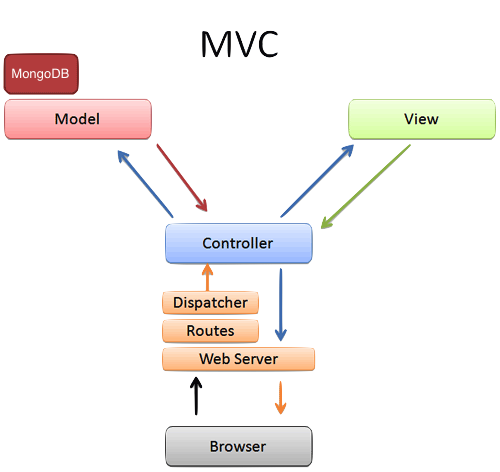
\includegraphics[width=\linewidth]{mvc-architecture-mongo}
     \caption{Patrón de diseño Modelo Vista Controlador (MVC)}\label{Fig:mvc}
   \end{minipage}
\end{figure}

	\begin{figure}[!htb]\centering
	   \begin {minipage}{1\textwidth}
	     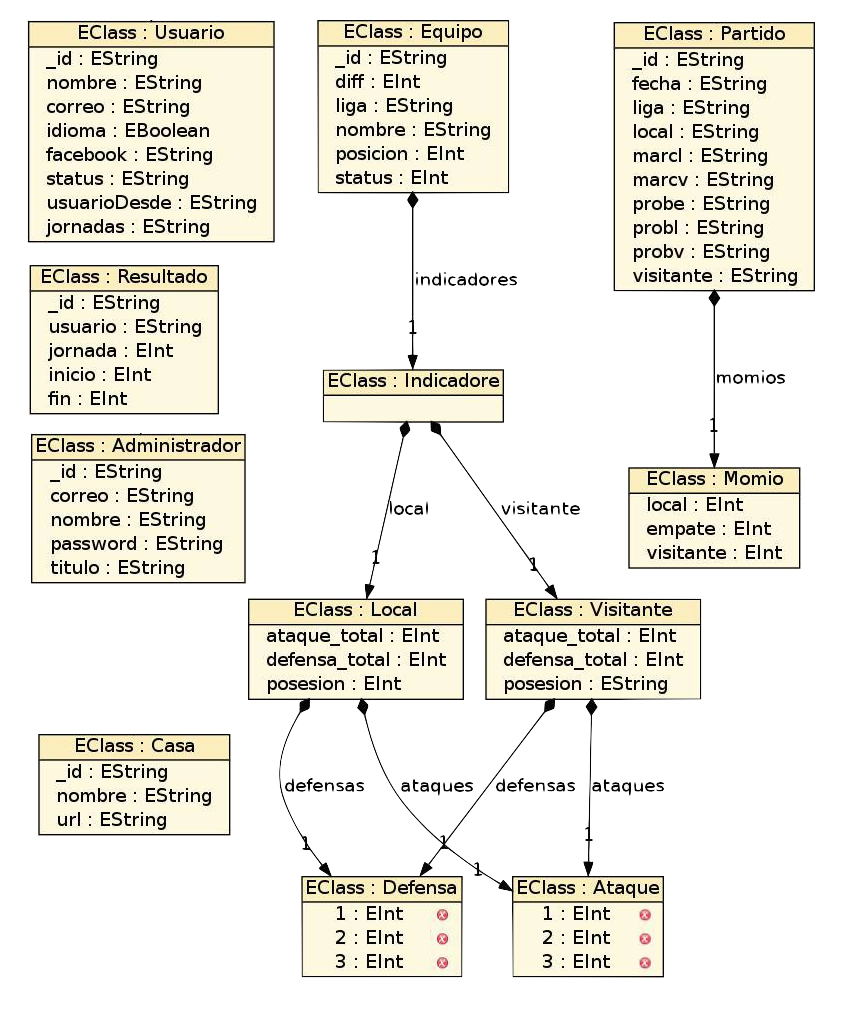
\includegraphics[width=\linewidth]{mongoDB/schema/bd-egobets}
	     \caption{Representación UML de las colecciones de la base de datos de Egobets}\label{Fig:db-egobets}
	   \end{minipage}
	\end{figure}

CodeIgniter es un framework\footnote{Es una estructura de software compuesta de componentes personalizables e intercambiables para el desarrollo de una aplicación. En otras palabras, un framework se puede considerar como una aplicación genérica incompleta y configurable a la que se le puede añadir las últimas piezas para construir una aplicación concreta \cite{upton2007codeigniter}.} de PHP que ahorra tiempo de programación, robustece cualquier sistema y permite al programador alcanzar un grado mayor de sofisticación en su código.

	De su página Web \cite{codeigniterWeb} se pueden destacar las siguientes propiedades:
	\begin{itemize}
		\item Tamaño pequeño. CodeIgniter 2.2 tiene una descarga 2.2MB, incluyendo la guía del usuario.
		\item Documentación clara. La guía que se incluye cuenta con guía y tutoriales para empezar a trabajar de manera muy práctica.
		\item Compatibilidad con casi cualquier servicio de alojamiento. Sólo necesita PHP 5.1.6 y tiene soporte con las bases de datos más comunes incluido MySQL.

		\item Casi no necesita configuración. Todas las variables y opciones de configuración vienen predefinidas a los estándares convenidos en internet.

	\end{itemize}


	Por la naturaleza de la arquitectura MVC es necesario conocer la definición de la estructura de datos para después poder describir en mayor detalle los elementos del sistema. Ahora, hay que recordar que Egobets no utiliza una base de datos relacional por lo que se presenta un diagrama de clases para representar las colecciones que se tienen en la base de datos de Mongo DB.
	\textbf{Definición de la base de datos}
	La base de datos cuenta con seis colecciones principales (Véase la figura~\ref{Fig:db-egobets}):

	\begin{itemize}
		\item Usuario. Se trata de los usuarios que se enrolan al sistema y utilizan los servicios de portal, como las asesorías de apuestas o las predicciones de los partidos.
		\item Administrador. Estos usuarios son los que tienen privilegios para ingresar al portal administrador y gestionar la información del sistema.
		\item Equipo. En esta colección se almacenan todos los equipos de las cinco ligas junto con la posición en la que se encuentra  y la fortaleza con la que cuenta en ese momento.
		\item Partido. Se guardan los partidos de las cinco ligas junto con los marcadores estimados y después los reales. De igual manera se tienen los momios de las casas de apuestas para ese partido.
		\item Casa. En esta colección se almacenan los datos de las casas de apuestas de las cuales se recuperan sus momios para hacer los cálculos de las asesorías de apuestas.
		\item Resultado. Aquí se guarda la cantidad de dinero que obtiene o pierde un usuario en cada jornada.
	\end{itemize}
	Como se puede observar, hay conexiones entre algunas clases. Esto se debe a que las colecciones que tiene MongoDB permiten objetos complejos, de tal manera que un objeto puede contener un arreglo de otros objetos. Para ver un ejemplo de los datos almacenados en la base de datos véase el Apéndice \ref{chap:dbs}.

	Con base en la estructura de datos definida, retómese el patrón de diseño MVC, la propiedad más interesantes de CodeIgniter. Este patrón fue descrito por el noruego Trygve Reenskaug en 1979, y facilita la descripción del sistema de Egobets de una manera más organizada \cite{upton2007codeigniter} \cite{alfredo2005ingenieria}. En los siguientes apartado se describirán  los componentes de Egobets en estas tres dimensiones.


		 \subsection{Modelos}

		La información representa el dominio del problema y la base de datos se abstrae como un conjunto de objetos sobre los cuales recaen todas la acciones. En el modelo, los objetos básico definidos, reflejan las colecciones de la base de datos y a través del conector de base de datos, el modelo modifica los documentos en la base de datos conforme sea requerido.
		En particular, ya se dijo que los datos del sistema de Egobets son los definidos en la figura~\ref{Fig:db-egobets} y la definición de los objetos se pueden ver en el Apéndice~\ref{chap:dbs}. Ahora, recordando que PHP no es un lenguaje cuyos paradigma (inicial) se orientara objetos\footnote{PHP es un lenguaje que soporta objetos, y en particular PHP5 integra más este paradigma, pero no es un lenguaje orientado a objetos. Por ejemplo, muchas de sus funciones principales no pertenecen a ningún objeto.}, los datos que tiene definidos en el modelo son completamente dependientes de la estructura de la base de datos, entonces los objetos utilizados por los modelos son exactamente los mismos definidos en la BD y extraídos con las consultas.

		Como lo menciona Upton en su libro \cite{upton2007codeigniter}, la parte más fundamental es el escribir operaciones ``ABCD''. Es necesario poder Agregar, Borrar, Cambiar y Desplegar la información de las colecciones de la bases de datos. Estas funciones, aunque conceptualmente fáciles de entender, son bastante complejas y escribirlas puede consumir mucho tiempo; sin embargo, son la base de un modelo bien definido, fácil de mantener y reutilizable.

		En concreto, para el portal público de Egobets las siguientes son las funciones utilizadas en los modelos:
		\begin{itemize}
			\item \emph{Usuarios}
				\begin{itemize}
					\item Agregar - A través del modelo, se permite crear un nuevo \emph{usuario} de la plataforma.
					\item Cambiar - Se pueden cambiar los detalles del perfil de un \emph{usuario}, así como las casas de apuestas a las que está suscrito, también es posible actualizar las jornadas ya pagadas del usuario.
					\item Desplegar - Se pueden obtener todos los datos de un usuario en función de su identificador o buscar algún texto en su perfil. También se pueden mostrar los amigos que tiene en Facebook \cite{facebookDocuWeb} en el sistema y las casas de apuestas a las que está suscrito en Egobets.
				\end{itemize}
			\item \emph{Resultados}
			\begin{itemize}
				\item Agregar - Se recibe la información de la cantidad de dinero ganada o perdida por cada usuario e inserta esta información en la colección de \emph{Resultados}.
				\item Desplegar - Se obtienen los \emph{resultados} de ganancias o pérdidas en función del usuario. También se genera la información base para hacer las gráficas de la evolución de dinero en el tiempo.
			\end{itemize}
			\item \emph{Transacciones}
				\begin{itemize}
					\item Agregar - Se permite iniciar e insertar una nueva \emph{transacción} a la base de datos con un estatus de pendiente de pago.
					\item Cambiar - Se puede cambiar y asignar un estatus de pagada junto con una fecha de pago a una \emph{transacción} a través de este modelo.
					\item Desplegar - Para algún usuario, se pueden obtener todas las \emph{transacciones} realizadas.
				\end{itemize}
			\item \emph{Equipos}
				\begin{itemize}
					\item Desplegar - El modelo  de \emph{Equipos} despliega todos los \emph{equipos} registrados en el sistema y estos pueden ser filtrados directamente por:  nombre, identificador o liga a la que pertenecen. También se despliegan los equipos favoritos por cliente.
				\end{itemize}
			\item \emph{Partidos}
				\begin{itemize}
					\item Desplegar - Se muestran todos los \emph{partidos} registrados en el sistema y se pueden filtrar por: el equipo que juega en ellos, el identificador del partido o la liga a la que pertenecen. También este modelo permite obtener las estrellas de cada partido, estas estrellas denotan la confiabilidad que tiene la predicción del resultado de ese partido.
				\end{itemize}
		\end{itemize}

		\subsection{Vistas}

		\graphicspath{{/Users/brunomedina/Dropbox/Tesis-Egobets/egobets-notas/resources/vistas/}}

		Las vistas reflejan el estado del modelo y corresponden a las interfaces que se le presentan al usuario para el manejo de la información. Por lo general, pueden existir múltiples vistas sobre un mismo modelo, por ejemplo puede existir una vista que despliegue un listado de  partidos por liga y al mismo tiempo existir una vista que muestre una gráfica con la cantidad de goles anotados por los equipos locales a través del tiempo. Estas vistas utilizan los mismos modelos, pero la información que despliega es completamente distinta y tiene fines diferentes.

		También una vista puede implementar varios modelos, es decir, mostrar información compleja compuesta por varios elementos de la base de datos. Un ejemplo sería una vista que presente los datos de un partido junto con las estadísticas generales de cada equipo y una gráfica representativa de la cantidad de dinero gastada por los usuarios en las distintas apuestas del partido.

		Las vistas que se tienen en el sistema se pueden enumerar de la siguiente manera:
		\begin{itemize}
			\item \emph{\textbf{Vistas relativas al perfil del usuario}}

			\begin{figure}[!htb]\centering
			   \begin {minipage}{0.7\textwidth}
			     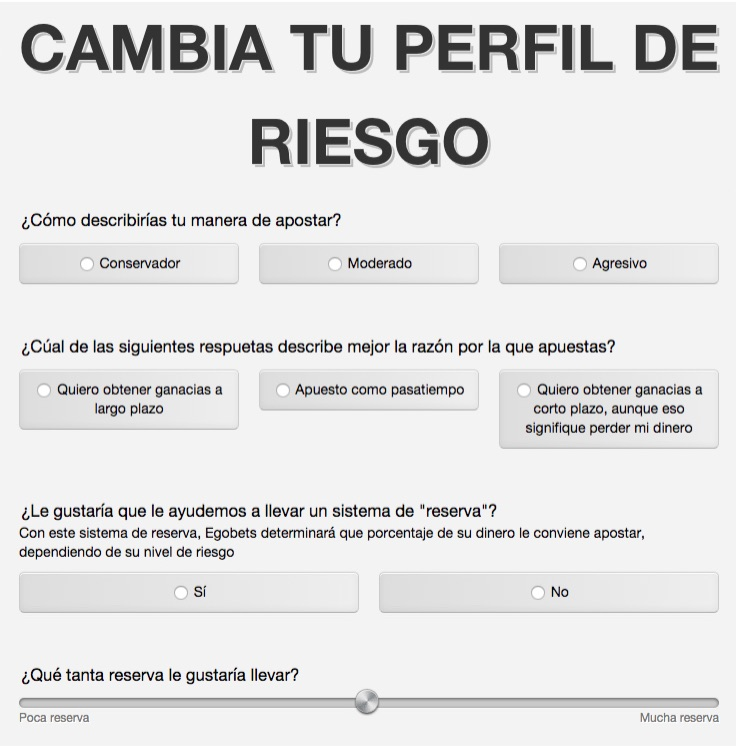
\includegraphics[width=\linewidth]{encuesta}
			     \caption{La encuesta define el perfil de riesgo del usuario}\label{Fig:encuesta}
			   \end{minipage}
			\end{figure}

			En este conjunto de vistas se le permite al usuario gestionar toda la información que tiene que ver con su perfil. Se tienen desde las pantallas para crear una cuenta, hasta las pantallas para editar la encuesta que define las recomendaciones que el usuario recibe.
			A continuación se enlistan estas vistas:
			\begin{itemize}
				\item Sign up. Permite al usuario crear una nueva cuenta para utilizar el sistema (Se puede utilizar Facebook \cite{facebookDocuWeb} para crear el perfil más rápidamente).
				\item Inicio de Sesión. A través de esta pantalla el usuario ingresa sus datos para entrar al sistema.
				\item Restablecer contraseña. Permite al usuario ingresar su correo electrónico para generar una nueva contraseña.
				\item Mi Perfil. En esta vista un usuario puede cambiar sus preferencias como el idioma, si requiere ser notificado cuando haya nuevas recomendaciones y seleccionar las casas de apuestas que utiliza.
				\item Mis Amigos. A través de esta pantalla se pueden ingresar los correos electrónicos de otras personas que tienen cuenta en Egobets para después comparar resultados de sus ganancias.
				\item Encuesta. Como ya se mencionó el riesgo del usuario depende de esta pantalla. El usuario puede ajustarla cada vez que guste cambiar su estrategia de apuesta. Ver imagen~\ref{Fig:encuesta}


			\end{itemize}


			\item \emph{\textbf{Vistas Estáticas}}



			Estas vistas no necesitan ser actualizadas casi nunca, es decir, su contenido es estático. Las páginas estáticas son:
			\begin{itemize}
				\item FAQ. Preguntas frecuentes que ayudan al usuario a comprender más a fondo el sistema (Ver imagen~\ref{Fig:faq}).

				\begin{figure}[!htb]\centering
				   \begin {minipage}{0.75\textwidth}
				     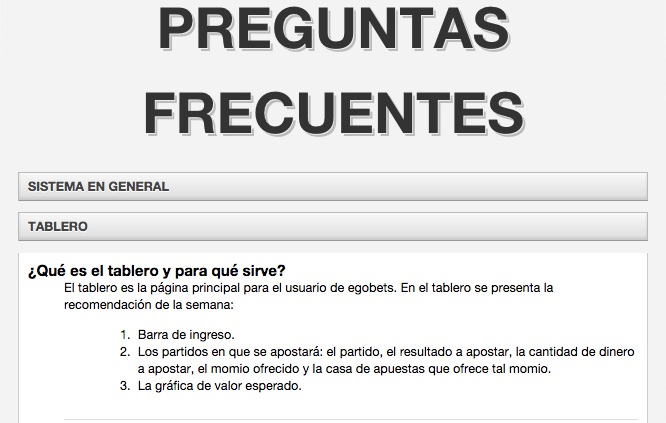
\includegraphics[width=\linewidth]{faq}
				     \caption{La encuesta define el perfil de riesgo del usuario}\label{Fig:faq}
				   \end{minipage}
				\end{figure}

				\item Home Page. La página que recibe a todos los que ingresan al sitio y presenta una bienvenida a los posibles clientes junto con una explicación de lo que es Egobets.com. Además de que contiene el aviso legal.
				\item Términos y condiciones. Presenta el contrato de uso al que se comprometen los clientes al utilizar el sistema.
			\end{itemize}


			\item \emph{\textbf{Vistas relativas a la operación del sistema}}


			En estas vistas se presenta la información de todas las ligas, equipos, partidos y las recomendaciones de apuestas.

			\begin{itemize}

				\item Tablero. La recomendación de apuestas de esta jornada es mostrada al usuario. Se le indica al usuario la cantidad de dinero en porcentaje a apostar en cada una de las apuestas recomendadas y los mejores momios para ese partido por casa de apuestas (Ver figura~\ref{fig:dashboard}).

				\begin{figure}[!htb]\centering
				   \begin {minipage}{0.9\textwidth}
				     \includegraphics[width=\linewidth]{dashboard}
				     \caption{Pantalla de inicio del usuario con recomendaciones de apuestas}\label{fig:dashboard}
				   \end{minipage}
				\end{figure}
				\item Mis Equipos. Una tabla con los equipos preferidos del usuario junto con sus variables de ataque y de defensa.
				\item Tabla de posiciones de la liga. Muestra los nombres de los equipos de la liga seleccionada, variables de ataque y defensa calculadas por el sistema  y el cambio en la tabla de posiciones que han tenido. Se permite al usuario agregar a sus favoritos cualquier equipo para tener un acceso directo a ellos.
				\item Detalle del Equipo. Se presenta el nombre del equipo, su posición en la liga y las estadísticas de ataque y defensa cuando es local o visitante. También se muestran el listado de los partidos próximos que tiene el equipo.
				\item Partidos de la jornada. Consiste en una tabla con los partidos próximos ordenados por fecha del juego. La tabla incluye los equipos participantes, quien es el favorito, el marcador esperado por el sistema y la fecha del juego.
				\item Detalle del partido. Se tienen los equipos que participan, el resultado más probable (junto con su confiabilidad en estrellas), el marcador esperado, la posesión del balón esperada y las estadísticas de ataque y defensa. Estas estadísticas se muestran divididas en las tres categorías. Medio centro, delanteros y definición, para el ataque. Y medio centro, defensas y portero, para la defensa. Cada una de estas variables despliega al ser presionada un histograma con la magnitud esperada de esa variable durante los noventa minutos del partido en intervalos de quince minutos. (Ver imagen~\ref{Fig:partido}).
				\begin{figure}[!htb]\centering
				   \begin {minipage}{0.8\textwidth}
				     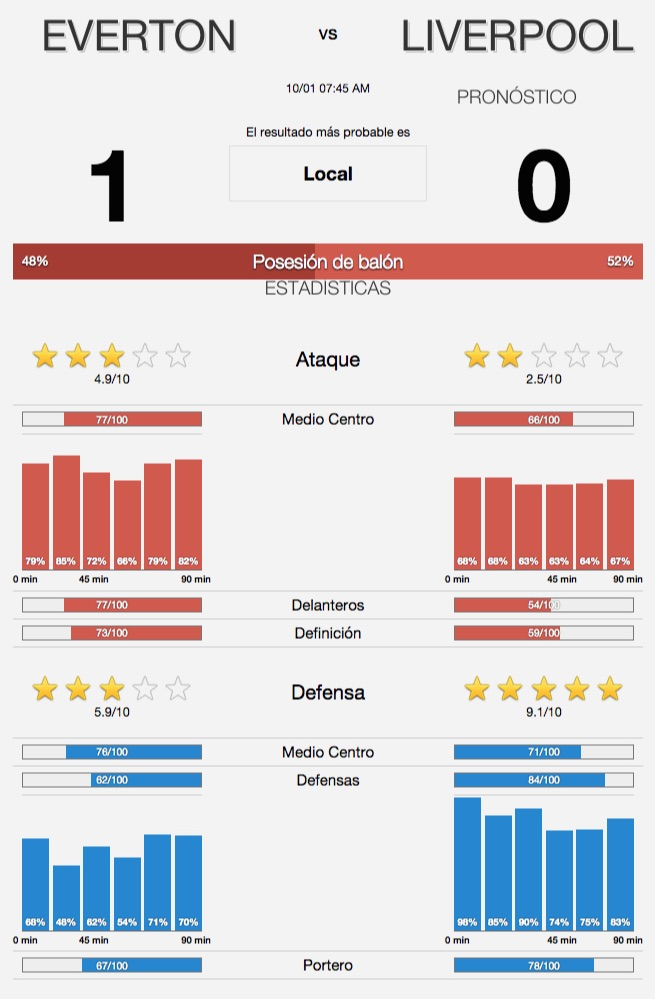
\includegraphics[width=\linewidth]{partido}
				     \caption{Partido con recomendación y estadísticas de los equipos}\label{Fig:partido}
				   \end{minipage}
				\end{figure}

				\item Partidos anteriores. Finalmente esta tabla muestra un comparativo de todos los partidos predichos y su resultado real. Se remarcan los aciertos del sistema y puede ser filtrada por liga.

			\end{itemize}

		\end{itemize}


		Todas la vistas descritas en los párrafos anteriores consisten en archivos HTML5\footnote{HTML viene de HyperText Markup Language, este lenguaje de marcado llegó a la versión 5 utilizada hoy en día el 24 de Octubre del 2014 en el consorcio de la World Wide Web (Básicamente el consorcio de Internet). Para más información leer What is HTML5 de MacLauhlin \cite{mclaughlin2011html5}.} creados dinámicamente en función del código PHP de las vistas. Cada una de estas pantallas cuentan con un archivo CSS\footnote{Cascade Style Sheet, } que aplica el estilo y el diseño al lenguaje de marcado HTML. A su vez, se utiliza Javascript para las animaciones, validaciones y cambios en las propiedades tanto del CSS como del HTML; un ejemplo claro del uso de Javascript es la animación de los gráficos de las estadísticas de los equipos.

		\subsection{Controladores}
		Corresponden a la manipulación de la información a través de sus diversas presentaciones, ofrecen opciones para cambiar el estado del modelo, son los encargados de consultar los modelos y proveer a las vistas los datos dinámicos a mostrar. Básicamente, los controladores implementan el comportamiento o el control de la lógica del sistema, especificando cuándo y como el sistema cambia de estado. Este comportamiento requiere la interacción de múltiples modelos y vistas.
		A continuación se muestra un listado de los controladores del sistema de Egobets junto con las funciones específicas que puede realizar cada uno de ellos.:
		\begin{itemize}
			\item \textbf{Usuario.}
			\begin{itemize}
				\item Restablecer/crear/cambiar un password de una cuenta de usuario.
				\item Calcular el perfil de riesgo del cliente realizando y procesando los resultados de la encuesta.
			\end{itemize}
			\item \textbf{Perfil.} Despliega la información completa del perfil de un usuario,
			\begin{itemize}
				\item Desplegar la información completa del perfil de un usuario junto con los botones necesarios para editarla.
				\item Agregar/quitar una cuenta de Facebook \cite{facebookDocuWeb} al perfil.
				\item Agregar/quitar casas de apuestas al usuario.
 				\item Desplegar información del historial de pagos del usuario.
				\item Agregar/quitar casas de apuestas al usuario.
			\end{itemize}
			\item \textbf{Dashboard.}
			\begin{itemize}
				\item Desplegar la información completa de la recomendación de apuestas de esta jornada al usuario en función de su perfil de riesgo, las casas de apuestas utilizadas y la reserva correspondiente a este usuario.
				\item Agregar la información de las ganancias o pérdidas del usuario en esta semana.
			\end{itemize}
			\item \textbf{Amigos.}
			\begin{itemize}
				\item Desplegar una tabla de posiciones del usuario entre sus amigos respecto a las ganancias de cada uno de ellos. También muestra el listado con la información de sus amigos.
				\item Agregar/quitar amigos de Facebook \cite{facebookDocuWeb} o por correo.
				\item Buscar amigos en el sistema con su correo electrónico.
			\end{itemize}
			\item \textbf{Ayuda.}
			\begin{itemize}
				\item Desplegar la información completa del perfil de un usuario junto con los botones necesarios para editarla.
				\item Agregar/quitar una cuenta de Facebook \cite{facebookDocuWeb} al perfil.
				\item Agregar/quitar casas de apuestas al usuario.
 				\item Desplegar información del historial de pagos del usuario.
				\item Agregar/quitar casas de apuestas al usuario.
			\end{itemize}
			\item \textbf{Sesión.}
			\begin{itemize}
				\item Desplegar la página de inicio de sesión.
				\item Iniciar la sesión del usuario con Facebook o a través de una combinación de correo y password.
				\item Cerrar la sesión de un usuario.
 				\item Crear un nuevo usuario desde cero o con Facebook \cite{facebookDocuWeb} login.
			\end{itemize}
			\item \textbf{Partido.}
			\begin{itemize}
				\item Desplegar la información de los resultados estimados para la jornada en curso.
				\item Desplegar la información de los partidos de la semana pasada con sus respectivos marcadores y las predicciones dadas por el sistema.
			\end{itemize}
			\item \textbf{Equipo.}
			\begin{itemize}
				\item Desplegar la tabla de los equipos favoritos del usuario.
				\item Desplegar las ligas disponibles en el sistema.
				\item Desplegar la tabla de posiciones con todos los equipos que juegan en una liga.
				\item Desplegar la pantalla de detalle de un equipo.
			\end{itemize}
			\item \textbf{Pagos.}
			\begin{itemize}
				\item Desplegar las opciones para comprar jornadas de recomendaciones.
				\item Procesar la transferencia correcta de parte de Paypal de los pagos realizados por el usuario.
			\end{itemize}
			\item \textbf{Ayuda.}
			\begin{itemize}
				\item Desplegar el archivo de preguntas y respuestas de manera correcta.
			\end{itemize}
			\item \textbf{Favoritos.}
			\begin{itemize}
				\item Agregar/Borrar equipos de los favoritos del usuario.
			\end{itemize}

		\end{itemize}

% Todas estas funciones realizadas por los controles definen por completo el sistema de Egobets. Es importante mencionar una función extra que se llama auth(); la cual corre en los constructores de cada uno de los controladores para asegurar que un usuario malintencionado no pueda realizar acciones a nombre de otro. Es decir, que si un usuario cuenta con una combinación válida de nombre de usuario y contraseña, el sistema, por ejemplo, no le permita obtener las ganancias que ha obtenido su peor enemigo en el sistema. De no contar con estas validaciones, se podría construir una llamada HTTP de tal manera que se pudiera obtener esta información.

Todas las funciones listadas en este capítulo conforman en su totalidad el sistema del portal público de egobets.com. Las funciones descritas en el capítulo 3 se ponen a disposición del usuario a través de las interfaces ya definidas y le proporcionan la recomendación de apuestas acorde a su perfil de riesgo. De igual manera, el usuario puede actualizar todos los datos necesarios de su perfil para generar recomendaciones más acorde a sus preferencias.

% En la siguiente sección de este documento, se retoma la función más interesante\footnote{Se considera más interesante una función que muestra recomendaciones de apuestas, que una función que permite al usuario cambiar el idioma del portal. El objetivo de esta tesis es el de mostrar una manera programática de obtener recomendaciones que permitan al usuario apostar de manera estratégica con el fin de obtener ganancias, no el de proveer documentación para la replicación de este sistema a través de ingeniería de software.} del sistema y se explica a mayor detalle su funcionamiento.


% \section{Servicio de asesoría de apuestas}
% \graphicspath{{/Users/brunomedina/Dropbox/Tesis-Egobets/egobets-notas/resources/}}
% \label{sec:service}
%
% En el Capítulo~\ref{chap:mate} se describió el algoritmo detrás de la generación de asesorías de apuestas desde un punto de vista teórico. En este apartado previo a las conclusiones, se hablará de como a través de varias herramientas se logra conseguir la información necesaria para presentarle al usuario una recomendación de apuestas como la de la figura~\ref{fig:dashboard}
%
% 				\begin{figure}[!htb]\centering
% 				   \begin {minipage}{0.9\textwidth}
% 				     \includegraphics[width=\linewidth]{vistas/dashboard}
% 				     \caption{Pantalla de inicio del usuario con recomendaciones de apuestas}\label{fig:dashboard}
% 				   \end{minipage}
% 				\end{figure}
%
% Como ya se mencionó, el algoritmo para generar la asesoría de apuestas se basa en los siguientes pasos:
%  \begin{enumerate}
%  	\item Determinación de apuestas redituables.
%  	\item Selección de apuestas de acuerdo al riesgo del cliente.
%  	\item Cálculo de la proporción del dinero a invertir por apuesta.
%  	\item Determinación del nivel de reservas.
%  	\item Presentar la recomendación.
%  \end{enumerate}
%
% Ahora en términos del sistema estos cinco pasos se llevan a cabo en milisegundos cada vez que el usuario entra a su perfil\footnote{En realidad se genera únicamente si no se tiene la recomendación ya guardada en el cache. Este caché se actualiza cada que hay cambios en los partidos, o cuando el usuario cambia su perfil de riesgo al contestar la encuesta nuevamente.}. Todo este laborioso trabajo que se definió con tanto esfuerzo en el Capítulo~\ref{chap:mate} se ve reducido a una librería de aproximadamente unas quinientas cincuenta líneas de código.
%
% En la sección~\ref{subsec:variables-necesarias} se habla de cuatro variables principales necesarias para poder realizar el algoritmo. Sin embargo, lo que es necesario para poder correr el sistema es: Obtener la información de los partidos, estimar las probabilidades de los partidos y generar las variables de riesgo en función de la encuesta. Estos serán los siguientes apartados del documento.
%
% \begin{figure}[!htb]\centering
%    \begin {minipage}{1\textwidth}
%      \includegraphics[width=\linewidth]{diagramas/sistemas}
%      \caption{Diagrama de herramientas y perfiles}\label{Fig:Sistemas}
%    \end{minipage}
% \end{figure}
%
% \subsection{Información de los partidos y pronósticos}
%
% Se desarrolló un sistema web que recupera al principio de cada temporada todos los partidos que se hayan jugado en las temporadas pasadas, así como el calendario de próximos partidos por jugar. Para lograr la extracción de esta información el sistema cuenta con un ``Web Scraper'' que consigue la información de la página de ESPN y la transforma en objetos que después son persistidos en la base de datos. Finalmente, esta información se organiza en un documento CSV para ser descargado por los administradores.
%
% El proceso que se lleva a cabo en el \emph{Back Office} para alimentar el \emph{Portal público} (Ver la figura~\ref{Fig:flujo}), se puede describir de la siguiente manera:
% \begin{enumerate}
% 	\item A través del \emph{Sistema de recopilación} los administradores descargan de la página de Internet de ESPN los resultados de todos los partidos de la temporada junto con la información de los próximos partidos por jugar  de cada una de las ligas Europeas.
% 	\item Los datos recopilados permiten a los administradores generar un conjunto de archivos de texto con toda la información de los resultados de los últimos partidos y las fechas de los próximos partidos.
% 	\item Los administradores usan estos archivos para alimentar el \emph{Sistema de estimación} y calcular los pronósticos de los próximos partidos y las probabilidades de los resultados.
% 	\item Se obtienen los archivos que contienen la información de los próximos partidos así como la información de los equipos por liga y su desempeño en la temporada en curso.
% 	\item En el \emph{Portal administrativo} se ingestan los archivos obtenidos con la información de los próximos partidos, resultados de partidos anteriores y las estadísticas de los equipos en la temporada en curso.
% 	\item Finalmente, con la nueva información ingresada, los usuarios podrán disfrutar en el \emph{Portal público} sus recomendaciones personalizadas de apuestas.
% \end{enumerate}
%
% \begin{figure}[!htb]\centering
%    \begin {minipage}{1\textwidth}
%      \includegraphics[width=\linewidth]{diagramas/flujo}
%      \caption{Proceso de alimentación del sistema}\label{Fig:flujo}
%    \end{minipage}
% \end{figure}
%
% \subsubsection{Web Scraper}
% El proceso de ``Web Scraping'' consiste en extraer y crear representaciones estructuradas con la información de un sitio Web en particular. HTML, el lenguaje de marcado usado para darle estructura a la información de las páginas web está sujeta a muchos cambios, especialmente cuando se actualiza su estilo. Ya que las técnicas de extracción se basan en el lenguaje de marcado, un solo cambio puede llevar a extraer datos incorrectos o incompletos \cite{cording2011algorithms}.
%
% Las técnicas de ``Web Scraping'' permiten, por ejemplo, que una compañía monitoree los precios de los productos de sus competidores. De igual manera le permiten a Egobets, conseguir la última información detallada con la información de las fechas de los partidos, marcadores, tiros a gol, posesión del balón y nombres de los equipos.
%
% Si el dueño de la información no provee de una API abierta, el remedio (como en el caso de Egobets) es el de escribir un programa que apunte a la información desplegada en la página Web. Las propiedades buscadas en un scraper son:
% \begin{itemize}
% 	\item Ser tan tolerante como pueda ser posible a cambios en el lenguaje de marcado.
% 	\item Ser lo suficientemente rápido como para ofrecer respuestas en milisegundos y evitar ``time-outs'' durante el consumo del servicio.
% 	\item No tener restricciones en los patrones que conforman la estructura del HTML del sitio. En específico esto implica que el servicio debe ser lo suficientemente bueno como para interpretar de la mejor manera la información aún incluso si el HTML se encuentra mal formado
% \end{itemize}
%
% Cording, P. \cite{cording2011algorithms} presenta en su tesis de maestría un estudio de como realizar un scraper que base su funcionamiento en la coincidencia aproximada de los patrones de un árbol, esta es la base de muchas de las librerías que existen (incluyendo la que se usa en este trabajo). Para realizar esta tarea se utiliza una librería de código abierto que permite manipular DOM\footnote{W3schools \cite{domWeb} lo define como: ``Documento W3C Object Model (DOM) es una interfaz de la plataforma y de lenguaje neutro que permite a los programas y scripts acceder y actualizar dinámicamente el contenido, la estructura y el estilo de un documento''. La especificación formal se puede leer en la recomendación \cite{wood1998document}.} de HTML y conseguir la información necesaria, esta libreria se llama: PHP Simple HTML DOM Parser.
%
% \textbf{Un ejemplo de uso}
%
% Supóngase el siguiente HTML:
%
% \lstset{language=HTML}
% \begin{lstlisting}[frame=single]
% <div class="team-names">
% 	<div class="team-name">
% 		<span>
% 			<img src="http://espncdn.com/teamlogos/soccer/500/102.png" alt="Villarreal" width="22">
% 			Villarreal
% 		</span>
% 	</div>
% 	<div class="team-name">
% 		<span>
% 			<img src="http://espncdn.com/teamlogos/soccer/500/93.png" alt="Athletic Bilbao" width="22">
% 			Athletic Bilbao
% 		</span>
% 	</div>
% </div>
% \end{lstlisting}
%
% Ahora analícese el siguiente código:
%
% \lstset{language=PHP}
% \begin{lstlisting}[frame=single]
% 	$aux = $table->find('.team-name',0);
% 	$nomEquipoLocal = $aux;
% 	$partido['prints']['local_nom']= $nomEquipoLocal;
% 	$idEspnEquipoLocal = trim(strstr(substr(strstr($aux->innertext, 'soccer/500/'), strlen('soccer/500/')),'.png',true));
% \end{lstlisting}
%
%
% Con este código se pueden obtener los nombres del equipo local y el identificador que le asigna ESPN a sus equipos. Esto es gracias a que \emph{``find('.team-name',0)''} recorre todo el árbol DOM y encuentra todas las ocurrencias de la clase con nombre \emph{``team-name''} el cero que se le proporciona a la función \emph{find} regresa el primer elemento encontrado. De ahí, la propiedad \emph{``->innertext''} muestra la cadena de caracteres plana que contiene ese elemento, por lo que basta con hacer un manejo de cadenas de caracteres para obtener el identificador del equipo que se nombra el archivo PNG del logo del equipo. Para más ejemplos y documentación de como utilizar la librería dirigirse a \cite{sourceparserWeb}.
%
%
% % \end{enumerate}
%
% \subsection{Generar las variables en función de la encuesta}




%
% \begin{enumerate}
% 	\item \emph{Recomendación personalizada de apuestas en fútbol:} Cada persona es diferente y debe ser tratada de forma única, en Egobets se determina el perfil de riesgo de cada usuario mediante una encuesta y se le recomienda apuestas a su medida, de tal forma que pueda obtener ganancias y sentirse cómodo al mismo tiempo.
% 	\item \emph{Pronósticos:} Para cada partido se proporcionan, entre otros: marcador final más probable, resultado más probable y el nivel de posesión de balón de cada equipo.
% 	\item \emph{Estadísticas:} A través de éstas se pueden analizar las fortalezas y debilidades de los equipos favoritos del usuario.
% \end{enumerate}
%
% \subsection{Encuesta}
% \label{subsec:encuesta}
%
%
% \textbf{Perfil de riesgo}
%
%
% El perfil de riesgo sirve para poder personalizar la asesoría de apuestas y se calcula a través de las respuestas proporcionadas en la encuesta de perfil de riesgo.
%
% De forma genérica hay tres perfiles de riesgo:
% \begin{enumerate}
% 	\item Agresivo: Toma riesgos altos para poder obtener la mayor cantidad de ganancias posibles en el corto plazo.
% 	\item Conservador: Apuesta a lo más seguro para proteger su dinero lo más posible, busca ganancias al largo plazo.
% 	\item Moderado: Término medio entre agresivo y conservador.
% \end{enumerate}
%
% \textbf{Sistema de reservas}
%
% En \emph{Egobets.com} se entiende que cada persona es diferente, que cada apuesta es diferente y debe ser analizada de forma individual, por eso se ha desarrollado el sistema de reservas que determina cuánto dinero apostar en la recomendación de la semana.
%
% La reserva es la cantidad de dinero que no se apostará, sirve para poder seguir apostando en semanas posteriores en el caso en que se lleguen a tener pérdidas.
%
%
% Se toman en cuenta tres factores: la volatilidad de la apuesta, la ganancia esperada de ésta y el nivel de riesgo deseado del cliente. Se combina esta información en un modelo probabilístico que proporciona la cantidad a apostar. Mediante este sistema se busca de proteger al cliente de pérdidas potenciales.
%
% Beneficios:
% \begin{enumerate}
%
% 	\item Protege su dinero de pérdidas potenciales.
% 	\item Permite recuperarse con mayor velocidad de semanas con pérdidas.
% 	\item Permite dar una estructura de fondo de inversión a las apuestas al obtener un sistema de interés compuesto.
%
% \end{enumerate}
%
% Costos:
% \begin{enumerate}
% 	\item Se restringe la cantidad de ganancias a corto plazo.
% \end{enumerate}
%
% Es un sistema a largo plazo, no se recomienda a personas que desean incurrir en riesgos elevados en beneficio de la posibilidad de obtener mayores ganancias.
%
%
% \subsection{Tablero de apuestas}
%
% El tablero es la página principal para el usuario de \emph{Egobets.com}. En el tablero se presenta la recomendación de la semana:
% \begin{enumerate}
%
% \item Barra de ingreso.
% \item Los partidos en que se apostará: el partido, el resultado a apostar, la cantidad de dinero a apostar, el momio ofrecido y la casa de apuestas que ofrece tal momio.
% \item La gráfica de valor esperado.
% \end{enumerate}
%
% En \emph{Egobets.com} se le da seguimiento a cada uno de nuestros clientes. Con esta información se puede monitorear la evolución del ingreso y así dar las recomendaciones de acuerdo al nivel de ganancias o pérdidas. Es importante que esta información sea verdadera para poder brindar el mejor servicio posible.
% \begin{enumerate}
%
% 	\item \textbf{¿Se pueden hacer recomendaciones de resultados que no sean los más probables?}
% \end{enumerate}
%
%
% Sí, depende del perfil de riesgo y de lo que pague la casa de apuestas en tal partido. En algunas ocasiones es recomendable apostar en contra del favorito si el pago es suficientemente grande. Si se tiene activado el sistema en contra de favoritos (en el menú perfil) o si el perfil es muy agresivo se presentarán muchas recomendaciones de este tipo.
%
% La gráfica de valor esperado es una herramienta visual que permite ver cuáles son los posibles resultados de la recomendación de la semana. En \emph{Egobets.com} se conoce que todas las apuestas tienen un riesgo y mediante esta gráfica se puede cuantificar: Cada barra representa la probabilidad de que se gane o pierda la cantidad indicada debajo de ella, mientras más grande sea la barra mayores probabilidades hay de que tal resultado ocurra.
%
%
%
% \subsection{Pronósticos}
% Pronósticos: Se pronostica el marcador final, la posesión del balón y el ganador del encuentro. Al poner el apuntador sobre el resultado más probable aparece el grado de confiabilidad del pronóstico.
%
%
% En \emph{Egobets.com} se presentan los equipos mediante un power ranking. Con base en las estadísticas de los partidos y dados sus resultados, se pronostica cuál será la tabla de posiciones al finalizar dicha liga.
%
%
% \subsection{Estadísticas}
%
%
% En orden de aparición: Una estrella indicando si el equipo está o no marcado como uno de los favoritos, la posición en el power ranking, el nombre del equipo, el índice de ataque general del equipo, el índice de defensa general del equipo y por último el cambio dentro de la tabla de power ranking.
%
% \begin{enumerate}
%
% \item Índice de ataque general: Con calificación de una a cinco estrellas o de uno a diez (abajo). Representa la capacidad general del equipo para atacar.
% \item Índices de medio centro, delanteros y definición: Con una calificación de cero a cien. Representan la capacidad de controlar el medio centro, de atacar a portería y de precisión de los tiros, respectivamente.
% \item Índice de defensa general: Con calificación de una a cinco estrellas o de uno a diez (abajo). Representa la capacidad general del equipo para defender.
% \item Índices de medio centro, defensas y portero: Con una calificación del cero a cien. Representan la capacidad de defender en el centro, de los defensas y del portero, respectivamente.
% \item Al hacer click en las variables mencionadas en 2 o 4 se tienen acceso a la evolución de tales variables desde el minuto 0 hasta el 90 de un partido.
% \end{enumerate}
%
% \begin{enumerate}
%
% 	\item \emph{Resultados de la jornada anterior:} Se presenta el partido, el marcador real, el marcador pronosticado y el resultado pronosticado. Esto con el fin de que los usuarios puedan comparar lo pronosticado y lo que en verdad ocurrió.
% 	\item \emph{Pronósticos de la jornada actual:} Se presenta el partido, el resultado pronosticado (o favorito), el marcador pronosticado y la fecha del encuentro. Además al poner el apuntador encima de un partido se presenta el grado de confiabilidad del pronóstico.
% \end{enumerate}
%
% Además para cada tabla se pueden presentar los resultados de una liga en particular al seleccionarla en el recuadro de arriba.
%
% \section{Alimentando el sistema}
% \label{sec:inserting-data}
%
% \begin{figure}[!htb]\centering
%    \begin {minipage}{1\textwidth}
%      \includegraphics[width=\linewidth]{sistemas}
%      \caption{Diagrama de sistemas y usuarios}\label{Fig:Sistemas}
%    \end{minipage}
% \end{figure}
%
% \begin{figure}[!htb]\centering
%    \begin {minipage}{1\textwidth}
%      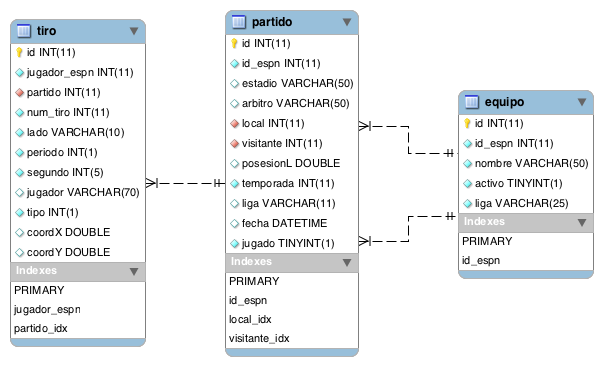
\includegraphics[width=\linewidth]{erd-pronosticos}
%      \caption{Diagrama de entidad-relación de la BD del recopilador}\label{Fig:erd-pronosticos}
%    \end{minipage}
% \end{figure}
%
% El proceso que se lleva a cabo en el \emph{Back Office} para alimentar el \emph{Portal público} (Ver la figura~\ref{Fig:flujo}), se puede describir de la siguiente manera:
% \begin{enumerate}
% 	\item A través del \emph{Sistema de recopilación} los administradores descargan de la página de Internet de ESPN los resultados de todos los partidos de la temporada junto con la información de los próximos partidos por jugar  de cada una de las ligas Europeas.
% 	\item Los datos recopilados permiten a los administradores generar un conjunto de archivos de texto con toda la información de los resultados de los últimos partidos y las fechas de los próximos partidos.
% 	\item Los administradores usan estos archivos para alimentar el \emph{Sistema de estimación} y calcular los pronósticos de los próximos partidos y las probabilidades de los resultados.
% 	\item Se obtienen los archivos que contienen la información de los próximos partidos así como la información de los equipos por liga y su desempeño en la temporada en curso.
% 	\item En el \emph{Portal administrativo} se ingestan los archivos obtenidos con la información de los próximos partidos, resultados de partidos anteriores y las estadísticas de los equipos en la temporada en curso.
% 	\item Finalmente, con la nueva información ingresada, los usuarios podrán disfrutar en el \emph{Portal público} sus recomendaciones personalizadas de apuestas.
%
% \begin{figure}[!htb]\centering
%    \begin {minipage}{1\textwidth}
%      \includegraphics[width=\linewidth]{flujo}
%      \caption{Proceso de alimentación del sistema}\label{Fig:flujo}
%    \end{minipage}
% \end{figure}
% \end{enumerate}
%
%


% \section{Descripción General}
% \label{sec:description}
%
% El ecosistema de Egobets consiste principalmente de cuatro piezas de software. Ver la figura~\ref{Fig:Sistemas}.
%
%
%
%
% \begin{figure}[!htb]\centering
%    \begin {minipage}{1\textwidth}
%      \includegraphics[width=\linewidth]{sistemas}
%      \caption{Diagrama de sistemas y usuarios}\label{Fig:Sistemas}
%    \end{minipage}
% \end{figure}
%
% El Sistema de recopilación de información y estadísiticas de los partidos (\emph{Sistema de recopilación}), el \emph{Portal administrativo} y el \emph{Portal público} corren bajo una arquitectura cliente servidor en la nube de Amazon Web Services; mientras que el Sistema de estimación de probabilidades (\emph{Sistema de estimación}) corre en un ordenador personal.
%
%

%
% \subsection{Piezas de software y su interacción}
%
% \begin{figure}[!htb]\centering
%    \begin {minipage}{1\textwidth}
%      \includegraphics[width=\linewidth]{flujo}
%      \caption{Diagrama de flujo de información}\label{Fig:flujo}
%    \end{minipage}
% \end{figure}
%
% El proceso que se lleva a cabo en el \emph{Back Office} para alimentar el \emph{Portal público} (Ver la figura~\ref{Fig:flujo}), se puede describir de la siguiente manera:
% \begin{enumerate}
% 	\item A través del \emph{Sistema de recopilación} los administradores descargan de la página de Internet de ESPN los resultados de todos los partidos de la temporada junto con la información de los próximos partidos por jugar  de cada una de las ligas Europeas.
% 	\item Los datos recopilados permiten a los administradores generar un conjunto de archivos de texto con toda la información de los resultados de los últimos partidos y las fechas de los próximos partidos.
% 	\item Los administradores usan estos archivos para alimentar el \emph{Sistema de estimación} y calcular los pronósticos de los próximos partidos y las probabilidades de los resultados.
% 	\item Se obtienen los archivos que contienen la información de los próximos partidos así como la información de los equipos por liga y su desempeño en la temporada en curso.
% 	\item En el \emph{Portal administrativo} se ingestan los archivos obtenidos con la información de los próximos partidos, resultados de partidos anteriores y las estadísticas de los equipos en la temporada en curso.
% 	\item Finalmente, con la nueva información ingresada, los usuarios podrán disfrutar en el \emph{Portal público} sus recomendaciones peronalizadas de apuestas.
% \end{enumerate}
%
%
% \subsection{Sistema de recopilación de información y estadísticas de los partidos}
% \graphicspath{{/Users/brunomedina/Dropbox/Tesis-Egobets/egobets-notas/resources/recopilador/}}
%
%
% \subsubsection{Tecnologías destacadas}
%
% \begin{itemize}
% 	\item \textbf{Servidor LAMP.} Esta es una de las configuraciones más populares para servidores web.
% 		Una de las principales ventajas de utilizar una arquitectura LAMP es que la mayoría del software utilizado corre bajo la ``Licencia Pública General de GNU'', esta licencia de uso permite a los programadores que utilizan este software, ser capaces de ver el código fuente y en muchos casos le permiten modificarlo y compartirlo \cite{lozano2008software}.
% 	El famoso acrónimo representa lo siguiente :
% 	\begin{itemize}
% 		\item Apache. El servidor HTTP, encargado de recibir y procesar las llamadas HTTP, nació hace diecisiete años como un proyecto por desarrollar un software robusto, de grado comercial, modular y gratuito para servir peticiones (Web) HTTP. Algunas de las ventajas con las que cuenta son \cite{apacheWeb}:
% 		\begin{itemize}
% 			\item Gran variedad de módulos. Existen muchos módulos que la comunidad desarrolla para atacar las problemáticas diarias, gracias a que su comunidad es muy activa estos desarrollos nunca acaban.
% 			\item Fácil de administrar. El soporte de la comunidad y su extensivo uso permite que sea muy sencillo encontrar documentación de como realizar las funciones básicas de administración de servidores como la creación de nuevos dominios, implantación de certificados SSL, etc.
% 			\item No importa el sistema operativo, Apache corre en UNIX, Windows, Mac y en la gran mayoría de sistemas operativos.
% 			\item Corre bajo la licencia pública general de GNU.
% 		\end{itemize}
%
% 		\item MySQL. Base de datos relacional que permite al sistema persistir toda la información recuperada del internet. Las principales características de MySQL son \cite{mysqlWeb}:
% 		\begin{itemize}
% 			\item Sistema de administración. El servidor MySQL provee las herramientas para agregar, ingresear, procesar y desplegar la información guardada en la base de datos.
% 			\item Las bases de datos MySQL son relacionales. La información se guarda en tablas separadas en vez de poner todo junto en un solo lugar. Las estructuras de base de datos están organizadas en archivos físicos optimizados para la velcidad. El modelo lógico con objetos como bases de datos, tablas, vistas, tuplas y columnas ofrece un ambiente de programación flexible. Y MySQL se asegura de que se respeten los tipos de relaciones entre tablas como puede ser uno a uno, uno a varios, únicas, u opcionales. Una base de datos bien diseñada nunca permitirá información incosistente, duplicada, huerfana, fuera de fecha o perdida.
% 			\item Corre bajo la licencia Pública General de GNU. Por lo que se puede modificar y ser utilizado por cualquiera.
% 		\end{itemize}
% 				\item PHP:
%
%
% 	\item Code Igniter. Es un framework\footnote{Es una estructura de software compuesta de componentes personalizables e intercambiables para el desarrollo de una aplicación. En otras palabras, un framework se puede considerar como
% una aplicación genérica incompleta y configurable a la que se le puede añadir las últimas piezas para construir una aplicación concreta.} de PHP que ahorra tiempo en le programación, robustece tu sistema y permite al programador alcanzar un grado mayor de sofisticación en su código. Uno de los puntos interesantes de este framework es que utiliza el patrón de diseño conocido como Modelo Vista Controlador (MVC), este patrón fue descrito por el noruego Trygve Reenskaug en 1979.
% 	Sobre el libro de Upton \cite{upton2007codeigniter} se tiene una aproximación a este patrón de diseño en CodeIgniter:
% 	\begin{itemize}
% 		\item Modelos, son objetos que representan los datos. Estos objetos reflejan las tabla de la base de datos y pueden modificarla conforme sea requerido. Los modelos también realizan operacioens a los datos según sea necesario.
% 		\item Vistas, reflejan el estado del modelo. Son las responsables de desplegar la información al usuario final. En este caso específico, todas las vistas son representaciones HTML del contenido.
% 		\item Controladores, ofrecen opciones para cambiar el estado del modelo. Son los encargados de consultar los modelos. Proveen a las vistas los datos dinámicos a mostrar.
% 	\end{itemize}
% 	De su página Web \cite{codeigniterWeb} se pueden destacar las siguientes propiedades:
% 	\begin{itemize}
% 		\item Tamaño pequeño. CodeIgniter 2.2 tiene una descarga 2.2MB, incluyendo la guía del usuario.
% 		\item Documentación clara. La guía que se incluye cuenta con guía y tutoriales para empezar a trabajar de manera muy práctica.
% 		\item Compatibildad con casi cualquier servicio de alojamiento. Sólo necesita PHP 5.1.6 y tiene soporte con las bases de datos más comunes incluído MySQL.
%
% 		\item Casi no necesita configuración. Todas las variables y opciones de configuración vienen predefinidas a los estandares convenidos en internet.
%
% 	\end{itemize}
%
%
% 	\item PHP Simple HTML DOM Parser
% 	Es un script de PHP que permite interpretar el HTML DOM de una página web y permite manipularlo de manera muy sencilla. Requiere PHP 5 o mayor, soporta archivos HTML mal formados y permite encontrar las etiquetas HTML con selectores como lo haría jQuery. Con una simple línea de código basta para extraer los contenidos de una página HTML \cite{htmlparserWeb}.
% 	\cite{chen2009php} \cite{chowdhury2014intelwiki}
% 	\item Bootstrap. Es un framework elegante, intuitivo y poderoso que agiliza y facilita el desarrollo Web de front-end Su principal objetivo es facilitar el desarrollo de sitios móviles y responsive.
% 	Documentación amplia y detallada, docenas de elementos HTML, componentes CSS e increíbles plugins de jQuery son algunas de sus principales características\cite{bootstrapWeb}.
% 	\cite{otto2010bootstrap}
% 	\cite{cochran2012twitter}
%
% \end{itemize}
%

% % Definir lo que es un scraper
% %
% %
% % Definir las páginas que se buscan y como se recorren
% %
% % Definir los objetos finales de la base de datos que se consumen.
% %
% %
%
%
% \subsubsection{Descripción de su funcionamiento}
%
% \begin{enumerate}
% 	\item \textbf{Equipos de la temporada.}
% 	Para poder comenzar la recuperación de información, es importante contar con los equipos que estén jugando esta temporada. Dependiendo de los resultados de la temporada anterior, los equipos que hayan quedado hasta abajo en la tabla de posición descienden a ligas menores y a su vez suben los mejores de estas ligas. Ver figura~\ref{Fig:los-equipos}
% 	\begin{figure}[!htb]\centering
% 	   \begin {minipage}{1\textwidth}
% 	     \frame{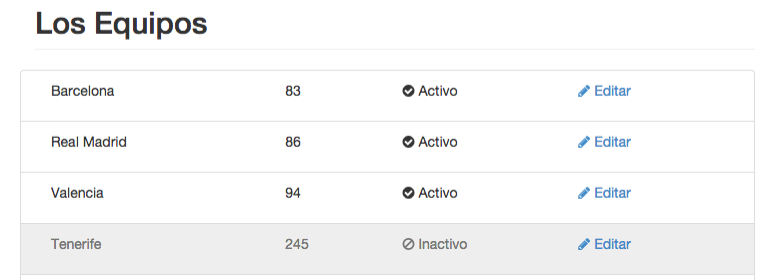
\includegraphics[width=\linewidth]{los-equipos}}
% 	     \caption[Ejemplo de equipos de la liga española]{Ejemplo de equipos de la liga española\footnotemark }\label{Fig:los-equipos}
% 	   \end{minipage}
% 	\end{figure}
%
%
% 	\item \textbf{Calendario de próximos partidos.}
% 	\begin{figure}[!htb]\centering
% 	   \begin {minipage}{1\textwidth}
% 	     \frame{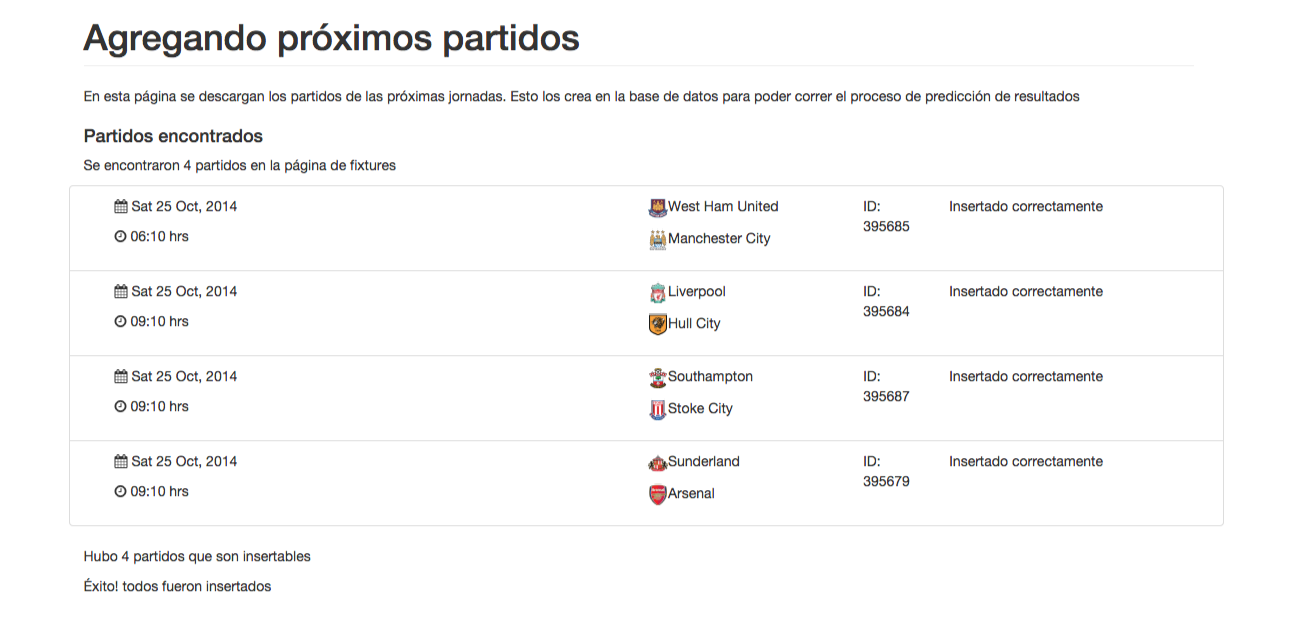
\includegraphics[width=\linewidth]{proximos-partidos}}
% 	     \caption{Recuperación de próximos partidos}\label{Fig:proximos-partidos}
% 	   \end{minipage}
% 	\end{figure}
%
% 	\item \textbf{Estadísticas e información de partidos jugados.}
% 	\begin{figure}[!htb]\centering
% 	   \begin {minipage}{1\textwidth}
% 	     \frame{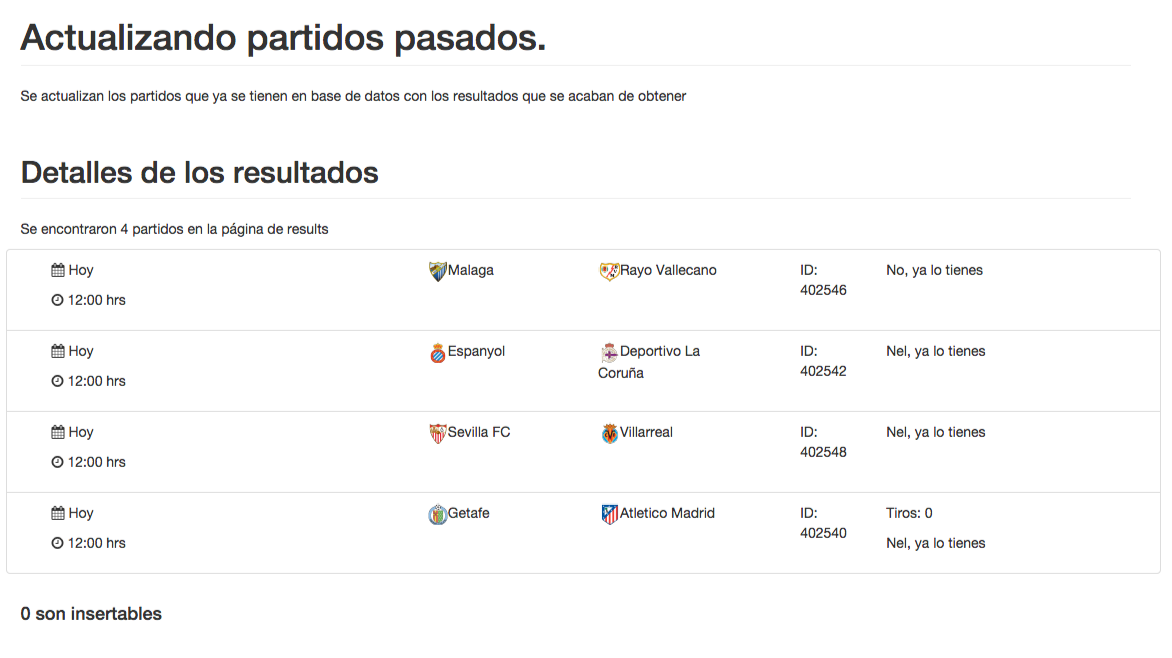
\includegraphics[width=\linewidth]{pasados-partidos}}
% 	     \caption{Recuperación de resultados de partidos ya jugados}\label{Fig:pasados-partidos}
% 	   \end{minipage}
% 	\end{figure}
% 	\item \textbf{Generación de archivos con resultados.}
% 	Es importante mencionar que se usan aproximadamente los últimos quinientos partidos para la generación de los archivos, esto implica que se deben tener en base de datos los equipos que participaron en las pasadas dos temporadas de juegos. Por este motivo de pueden encontrar equipos que se encuentran en el sistema con la bandera de inactivos.
%
% \end{enumerate}
%
%
%
%
%
%
%
%
%
%
%
%
%
% \subsection{Sistema de estimación de probabilidades}
% Adicionalmente en esta sección se describirá el funcionamiento del Sistema de Estimación. Sin embargo, al ser un conjunto de programas en \emph{Fortran} que son ajenos al autor, no se profundizará en los detalles del desarrollo del mismo. Sin embargo, se dará la pauta para entender como se podrían generar probabilidades y pronósticos de los partidos.
%
% \subsubsection{Predicciones}
%
%
%
% \cite{rue2000prediction}
%
% \cite{baio2010bayesian}
%
% \cite{dixon2004value}
%
% \cite{koopman2013dynamic}
%
%  \subsubsection{Tecnologías destacadas}
%
% \begin{itemize}
% 	\item \textbf{Fortran}
% 	\cite{robison1996c++}
% 	\cite{veldhuizen1997will}
% \end{itemize}
%
% \subsubsection{Descripción de su funcionamiento}
%
% Montecarlo
% Poisson
% Nonormal
% Markov
%
%
% \subsection{Portal administrativo}
%
% \subsubsection{Sitio web para los administradores}
%
%  \cite{alfredo2005ingenieria}
%
%  \subsubsection{Tecnologías destacadas}
%
%  \begin{itemize}
%  	\item LNNP
%  	\item Code Igniter
%  	\item Raphael
%  \end{itemize}
%
%  \subsubsection{Diagrama de base de datos}
%
%  \subsubsection{Descripciónde su funcionamiento}
%
%  \begin{itemize}
%  	\item CRUD
%  	\item Ingesta de archivos
%
%  \end{itemize}
%
%
% \section{Portal público Egobets.com}
%
% \subsection{Características principales}
% \subsubsection{Sitio web para los jugadores}
% \subsubsection{Tecnologías destacadas}
%
%  \begin{itemize}
%  	\item LNNP
%  	\item Code Igniter
%  	\item Parallax
%  \end{itemize}
%
% \subsubsection{Módulos}
%
%  \begin{itemize}
%  	\item Tablero
%  	\item Mis Equipos
%  	\item Ligas
%  	\item Partidos
%  	\item Perfil
%  	\item Pagos
%  	\item Perfil de riesgo
%  	\item Sistemas de reserva
%  \end{itemize}
%
%
%
 %Conclusiones
% Reestructurando a sólo 4 capítulos
%% \chapter{Portal público}
% \section{Perfil de usuario}
% \section{Encuesta de adversidad al riesgo}
% \section{Ahorro precaucional}
% \section{Sugerencia de apuestas}
% \section{Pagos en línea}
% \section{Power ranking}
%
\chapter{Conclusiones}

En esta tesis se describió el sistema de recomendación de apuestas personalizadas para las ligas europeas de futbol: Egobets, una aplicación de las matemáticas a la computación. De este trabajo se puede concluir lo siguiente:



\begin{itemize}


	\item Existe más de un modelo que permita predecir los resultados de los partidos de las ligas europeas de futbol. Más aún, el modelo de Maher (1982)\cite{maher1982modelling} proporciona predicciones lo suficientemente confiables como para considerar su uso en una estrategia de apuestas de hoy en día.

	\item Conociendo las probabilidades de los partidos, aún siendo estimadas, es posible encontrar una estrategia de apuestas que genere rendimientos positivos. Por ejemplo, Koopman en su artículo \cite{koopman2013dynamic} expone un ejemplo donde, mediante una estrategia de apuestas simple, por cada $75$ unidades apostadas recibe $25$ unidades de ganancia.

	\item La adversidad al riesgo de un apostador se puede modelar con funciones de utildad, esto permite que las recomendaciones de apuestas sean personalizadas y hagan sentir al usuario cómodo mientras apuestan.
	
	\item Considerando que las temporadas del futbol tienen varias jornadas, se integra un sistema de reservas cuya función principal consiste en maximizar la tasa de crecimiento de las ganancias del jugador. Vancura \cite{vancura2000finding} muestra varias estrategias de reservas que buscan conseguir estos resultados.

\item En el sistema de Egobets.com se provee de una asesoría de apuestas integral para cada semana de la temporada donde se utilizan las predicciones de los resultados de los partidos, el perfil de riesgo del usuario y el sistema de reservas.

\item Los momios que publican las casas de apuestas se enfocan a predecir el mercado, por lo tanto se pueden mejorar las probabilidades propuestas.

\item  El porcentaje de aciertos en los pronósticos es del $70\%$ para la liga española, $61\%$ en la italiana, $52\%$ en la inglesa, $52\%$ en la alemana y $48\%$ en la francesa.

\item En los resultados observados, Egobets reporta un rendimiento desde el $29\%$ hasta el $83\%$ dependiendo del nivel de riesgo por apuesta del usuario.

\item El computo en la nube es esencial para los sistemas como Egobets, sus ventajas como escalabilidad permiten mantener costeables y funcionales los servicios.

\item El enfoque de un desarrollo al diseño y la usabilidad permiten que el usuario se enfoque en realizar únicamente lo que debe realizar.

\item MongoDB proporciona el beneficio de guardar información sin una estructura definida. Esto permite mucha mayor flexibilidad en los documentos que se persisten y la información que contienen\cite{puniaimplementing}.

\end{itemize}

% - Los juegos de azar de los casinos contemplan un margen para la casa que les garantiza ganancias a futuro.
% - Es claro que, más allá del azar, la habilidad y destreza de los equipos dominan los resultados de una temporada de futbol.
% - Los momios que publican las casas de apuestas se enfocan a predecir el mercado, por lo tanto se pueden mejorar las probabilidades propuestas.
% - Existe más de un modelo que permita predecir los resultados de las ligas de futbol, desde Maher \cite{maher1982modelling} estas predicciones han sido lo suficientemente confiables como para considerar su uso en apuestas.
% - Conociendo las probabilidades de los partidos, aún siendo estimadas, es posible encontrar una estrategia de apuestas que genere rendimientos positivos como demostró Koopman en su artículo \cite{koopman2013dynamic} mediante una simple estrategia de apuestas considerando valores esperados positivos.
%
%
% - Además de tener las probabilidades y la estrategia de apuestas, Vancura \cite{vancura2000finding} señala que el criterio de Kelly \cite{kelly1956new} maximiza asintóticamente la tasa de crecimiento de las ganancias, por lo que se integra esquema de reservas a la solución propuesta.
%
% - Con el fin de buscar una asesoría personalizada se propone un esquema de recomendaciones basadas en el perfil de riesgo del apostador.
%
% - En el sistema de Egobets.com se provee de una asesoría de apuestas integral para cada semana de la temporada donde se utilizan las predicciones de los resultados de los partidos, el perfil de riesgo del usuario y el sistema de reservas.
%
%
% - El porcentaje de aciertos en los pronósticos es del $70\%$ para la liga española, $61\%$ en la italiana, $52\%$ en la inglesa, $52\%$ en la alemana y $48\%$ en la francesa.
%
%
% - En los resultados observados, Egobets reporta un rendimiento desde el $29\%$ hasta el $83\%$ dependiendo del nivel de riesgo por apuesta del usuario.
%
% - Las ganancias dependen del acierto de las predicciones, sin embargo tener estas ganancias con la probabilidad de aciertos que se tiene verifica las sospechas de que se puede tener una estrategia redituable de apuestas a pesar del pronóstico de los partidos.
%
% - El computo en la nube es esencial para los sistemas como Egobets, sus ventajas como escalabilidad permiten mantener costeables y funcionales los servicios.
%
% - El enfoque de un desarrollo al diseño y la usabilidad permiten que el usuario se enfoque en realizar únicamente lo que debe realizar
%
% - MongoDB proporciona el beneficio de guardar información sin una estructura definida. Esto permite mucha mayor flexibilidad en los documentos que se persisten y la información que contienen\cite{puniaimplementing}. Mientras que las bases de datos relacionales resultan mucho más eficientes en consultas complejas. En general, un esquema combinado de ambos tipos de bases de datos pueden resultar en un sistema de información eficaz y completo \cite{faraj2014comparative}.
%
%
% Beneficios:
%
% - Egobets ofreca recomendaciones personalizadas de apuestas, cada persona es diferente y es tratada de forma única. Gracias a la encuesta se determina el perfil de riesgo del usuario y se le asesora de tal manera que obtenga ganancias y se sienta cómodo  al mismo tiempo.
%
%
% Acciones a futuro
% - Mejorar el sistema de predicción de resultados.
% - En un futuro este sistema podría modificarse para abarcar más mercado.
% 	- Otras ligas, por ejemplo la mexicana
% 	- Otros deportes, por ejemplo futbol americano.
% - Incluso se varios de los autores hablan de que modelos parecidos a estos podrían servir para predecir elecciones.
%



\textbf{Acciones a futuro}
Un sistema tan complejo como este genera muchas áreas de oportunidad, una de ellas sería implementar las nuevas investigaciones para ejorar el sistema de predicción de resultados, otro detalle sería encontrar las funciones de utilidad más prolíficas del sistema y centrar a los usuarios sobre esas. Adicionionalmente, se podría trabajar en hacer más autónomo el sistema para generar las recomendaciones. Finalmente, sobre este sistema se podría incluso podrían modificar la lógica y adaptar el modelo para abarcar más mercados, como:
\begin{itemize}

	\item Otras ligas, por ejemplo la mexicana.

		\item Otros deportes, por ejemplo futbol americano.

	\item Incluso se varios de los autores hablan de que modelos parecidos a estos podrían servir para predecir elecciones.

\end{itemize}



%
Partiendo de los siguientes dos supuestos: a) un jugador promedio busca maximizar las ganancias de sus apuestas en función de su adversidad al riesgo y, b) apostar siempre conviene más que no apostar. Se plantea una manera de encontrar la apuesta óptima para un partido. Con base en este planteamiento se sigue el análisis a una jornada: ¿A qué partidos de la jornada el usuario le debería apostar? Finalmente, considerando que el usuario busca apostar en todas las jornadas de la temporada, se ataca el problema de la evolución del dinero a apostar durante toda la temporada.


\section{Ahorro precaucional}



\section{Evolución de la cantidad a Apostar}


%----------------------------------------------------------------------------------------
%	APÉNDICES
%----------------------------------------------------------------------------------------

\addtocontents{toc}{\vspace{2em}} % Agrega espacios en la toc

\appendix % Los siguientes capítulos son apéndices
%  Incluye los apéndices en el folder de apéndices
\chapter{La ruina del jugadorl}\label{chap:ruina}

http://www.columbia.edu/~ks20/stochastic-I/stochastic-I-GRP.pdf


http://www.ifp.illinois.edu/~sgorant2/gambler.html


Two gamblers Alice and Bob play the following game: Alice repeatedly tosses a fair coin. 
After each toss that comes up H, Bob pays Alice one dollar. After each toss that comes up T, 
Alice pays Bob one dollar. The game continues until either one or the other gambler runs out o
f money. If Alice starts with \$A and Bob starts with \$B,
. What is the probability that, when the game ends, Alice has all the cash?
. What is the expected duration of the game?
 
== Solution
Lets solve the problem using the Doob's Optional stopping Theorem for martingales.
Let $X_1,X_2,\cdots$ be the increments of Alice's wealth. Hence $X_i= 1$, depending on H or T. 
Hence, change in Alice's cash is
\( 
S_n = \sum_{i=1}^n X_i 
\)
Define  
\(
\tau = \min\{t: S_t = +B \mbox{ or } S_t = -A \}
\)
Clearly $\tau$ is a stopping time relative to the natural filtration
$\mathcal{F}_n = \sigma(X_1,X_2,X_3,\cdots,X_n)$. 
$\tau' = \tau \wedge n$ is also a stopping time.

=== (1) Probability of Alice winning
The sequence $S_n$ is a martingale relative to the natural filtration $\mathcal{F}_n$. 
Hence, using Optional Stopping Theorem for $n < \infty$,
\( 
 0 = {E}[S_0] = {E}[S_{\tau \wedge n}] = -A P(\tau \leq n \mbox{ and } S_{\tau} = -A) + B P(\tau \leq n \mbox{ and } S_{\tau} = +B) + E[S_n \chi_{\tau > n}]
 \)                                               
 As $n \to \infty$, the probability that  $\tau > n$ converges to zero. 
 The last term in the above equation is the expectation of a bounded martingale $S_n$
 bounded between $A$ and $B$ and converges to 0. Thus,
 \(
  0 = - A P(S_{\tau} = -A) + B P(S_{\tau} = +B) 
 \)
 Hence, probability that Alice has all the cash $S_{\tau} = +B$ is
 \(
 P(S_{\tau} = +B) = \frac{A}{A+B}.
 \)
 
=== (2) Expected duration of game.
The sequence $(S_n^2-n)$ is a martingale relative to the natural filtration $\mathcal{F}_n$.
Hence, using Optional Stopping Theorem for $n < \infty$,
\( 
 0 = {E}[S^2_0] = {E}[S_{\tau \wedge n}^2 - (\tau \wedge n)]
 \)                                                                                                          
 As $n \to \infty$, the probability that  $\tau > n$ converges to zero. 
Hence,
\(
E[\tau] = E[S_{\tau}^2] = A^2  P(S_{\tau} = -A) + B^2  P(S_{\tau} = +B) = AB 
\)                               
Hence, the expected duration of the game is AB.
\chapter{Formatos de archivos para la ingesta en el Portal de Administrativo}\label{chap:archivos}

Los tipos de archivos que el sistema procesa son archivos de texto plano, en codificación UTF-8 con ó sin BOM, en formato CSV, en el que la separación de valores se logra mediante tabulaciones, ó el caracter ``\textbackslash t'', y cada línea se termina con el caracter de nueva línea de Unix, es decir ``\textbackslash n''; el archivo debe contener todos los campos y estar en el orden indicado.

Con esto en mente, todas las variables presentadas aquí deberán ser escritas en el mismo renglón separadas por comas. Se ordenan en dos columnas únicamente para el ahorro de espacio.

\section{Formato de archivo para Partidos}

\begin{multicols}{2}
	\begin{enumerate}
	    \setlength{\itemsep}{1pt}
	    \setlength{\parskip}{0pt}
	    \setlength{\parsep}{0pt}
		\item Identificador único del equipo local,
		\item Identificador único del equipo visitante,
		\item Marcador local,
		\item Marcador visitante,
		\item Probabilidad local,
		\item Probabilidad empate,
		\item Probabilidad visitante,
		\item Fecha del partido, expresada en segundos desde la época Unix (1 de enero
		de 1970) en UTC.
	\end{enumerate}
\end{multicols}

\section{Formato de archivo para Equipos}
\begin{multicols}{2}
	\begin{enumerate}
	    \setlength{\itemsep}{1pt}
	    \setlength{\parskip}{0pt}
	    \setlength{\parsep}{0pt}
		\item Identificador único del equipo, 
		\item Variable local 1,
		\item Variable local 2,
		\item Variable local 3,
		\item Variable local 4,
		\item Variable local 5,
		\item Variable local 6,
		\item Variable local 7,
		\item Variable de ataque 1-1, 
		\item Variable de ataque 1-2,
		\item Variable de ataque 1-3, 
		\item Variable de ataque 1-4, 
		\item Variable de ataque 1-5, 
		\item Variable de ataque 1-6, 
		\item Variable de ataque 1-1, 
		\item Variable de ataque 1-2, 
		\item Variable de ataque 1-3, 
		\item Variable de ataque 1-4, 
		\item Variable de ataque 1-5, 
		\item Variable de ataque 1-6,
		\item Variable de ataque 2-1,
		\item Variable de ataque 2-2,
		\item Variable de ataque 2-3,
		\item Variable de ataque 2-4,
		\item Variable de ataque 2-5, 
		\item Variable de ataque 2-6, 
		\item Variable de ataque 3-1, 
		\item Variable de ataque 3-2, 
		\item Variable de ataque 3-3, 
		\item Variable de ataque 3-4, 
		\item Variable de ataque 3-5, 
		\item Variable de ataque 3-6, 
		\item Variable de defensa 1-1, 
		\item Variable de defensa 1-2, 
		\item Variable de defensa 1-3, 
		\item Variable de defensa 1-4, 
		\item Variable de defensa 1-5, 
		\item Variable de defensa 1-6, 
		\item Variable de defensa 1-1,
		\item Variable de defensa 1-2, 
		\item Variable de defensa 1-3, 
		\item Variable de defensa 1-4, 
		\item Variable de defensa 1-5, 
		\item Variable de defensa 1-6, 
		\item Variable de defensa 2-1, 
		\item Variable de defensa 2-2, 
		\item Variable de defensa 2-3, 
		\item Variable de defensa 2-4, 
		\item Variable de defensa 2-5, 
		\item Variable de defensa 2-6, 
		\item Variable de defensa 3-1, 
		\item Variable de defensa 3-2, 
		\item Variable de defensa 3-3, 
		\item Variable de defensa 3-4, 
		\item Variable de defensa 3-5, 
		\item Variable de defensa 3-6, 
		\item Variable de posesión
	\end{enumerate}
\end{multicols}

\graphicspath{{/Users/brunomedina/Dropbox/Tesis-Egobets/egobets-notas/resources/marco/}}

\chapter{Ligas europeas de fútbol}\label{chap:equipos}
En esta sección se presenta información relevante de cada una de las ligas europeas de fútbol. Esta información hace más comprensible los procesos de calificació y eliminación de los equipos. También se da un listado de los equipos participantes de las ligas.


\section{Bundesliga (Alemania)}


Fundada el 28 de Julio de 1962 en la convención anual de la \emph{DFL Deutsche Fußball Liga GmbH}, la primer temporada se jugó en 1963. La liga evolucionó en función de la reunificación de Alemania y la integración de la liga del Este \cite{hesse2003tor} Hoy en día la \emph{Bundesliga} es conocida como una de las ligas con mayor afluencia en sus partidos, en la temporada 2011/12 hubo un promedio de 44,293 espectadores por partido. Se vendieron 18.8 millones de entradas en total.

\begin{figure}[!htb]\centering
   \begin {minipage}{0.4\textwidth}
     
\includegraphics[width=\linewidth]{logo-bundesliga}
   \end{minipage}
\end{figure}
\begin{chapquote}{Gary Lineker, \textit{ex-futbolista inglés.}}
	``El fútbol es un deporte que inventaron los ingleses, que lo saben jugar los brasileños y en el que siempre ganan los alemanes.''
\end{chapquote}


La \emph{DFL} se encarga de la operación de las ligas de fútbol: \emph{Bundesliga} y \emph{2. Bundesliga}; que son las más importantes de Alemania. Cuenta con treinta y seis clubs de fútbol los cuales juegan se dividen en ambas divisiones (Ver~\ref{sec:equipos-ger}) Todos miembros de la Asociación  de la Liga cuentan con una licencia\footnote{Cada temportada todos los clubs deben cumplir los criterios deportivos, legales, administrativos, financieros y de infraestructura del Lizenzierungsordnung (LO) y sus respectivos apéndices} para poder jugar y deben seguir los sistemas de entrenamiento y procedimientos disciplinarios.

Dieciocho equipos juegan en cada división, cada equipo juega una vez de local y otra de visitante contra cada uno de los otros diecisiete equipos de la liga. Esto significa que al ser $n=18$ equipos se tienen $\sum\limits_{i=1}^{n-1} i= \sum\limits_{i=1}^{17} i= 153 $ partidos en una temporada. Al término de estos partidos se calculan los puntos que cada equipo tiene y se hace la tabla de posiciones, los dos peores equipos de la \emph{Bundesliga} son intercambiados con los dos mejores de la \emph{2. Bundesliga}. Mientras que el tercer mejor equipo de la \emph{2. Bundesliga} disputa un partido con el tercer peor equipo de la \emph{Bundesliga} para decidir quien se queda en la primera división. Análogamente, el equipo con más puntos se vuelve el campeón de la liga.

Los puntos de la tabla son dados por las victorias de cada equipo, una victoria suma tres puntos a la tabla; las derrotas o empates no suman nada. Si en la tabla hay equipos con la misma cantidad de puntos, para el desempate se deben consideran criterios como: diferencias de goles, cantidad de goles anotados en la temporada,  diferencia de goles que resulten de los partidos jugados entre ellos y la cantidad de goles como visitantes. Si todos estos criterios no deciden el desempate, se deberá jugar un partido en una cancha neutral para decidir su posición en la tabla.

La regulación de la cantidad de jugadores extranjeros en los equipos sigue la regulación d ela UEFA desde el 21 de Diciembre del 2005. Actualmente hay 977 jugadores con un contrato profesional, 503 en la \emph{Bundesliga} y 474 en la \emph{2. Bundesliga}. El cuarenta y siete por ciento de la primera división son extranjeros (234 jugadores) y el treinta y seis por ciento  en la segunda liga (171 jugadores)

En total, 43 clubs han ganado la Bundesliga desde su fundación. Los tres equipos con más campeonatos son: \emph{FC Bayern Munich} con 23 títulos, \emph{BFC Dynamo Berlin} con 10 y \emph{1. FC Nürnberg} con 9. Los tres máximos goleadores de la liga son: \emph{Ger Müller} (1965-1979) con 365 goles, \emph{Klaus Fischer} (1968-1988) con 268 y \emph{Jupp Heyncke}s con 220. \cite{bundesliga}


\subsection{Equipos Alemanes}
\label{sec:equipos-ger}
\begin{multicols}{2}
	\begin{itemize}
	    \setlength{\itemsep}{1pt}
	    \setlength{\parskip}{0pt}
	    \setlength{\parsep}{0pt}

		\item 1. FC Kaiserslautern

		\item 1. FC Köln GmbH \& Co.KGaA

		\item 1. FC Nürnberg

		\item 1. FSV Mainz 05

		\item Bayer 04 Leverkusen Fußball GmbH

		\item Borussia Dortmund GmbH \& Co. KGaA

		\item Borussia VfL 1900 Mönchengladbach GmbH

		\item DSC Arminia Bielefeld GmbH \& Co. KGaA

		\item Eintracht Frankfurt Fußball AG

		\item FC Augsburg 07

		\item FC Bayern München AG

		\item FC Carl Zeiss Jena e.V.

		\item FC Energie Cottbus

		\item FC Erzgebirge Aue

		\item FC Hansa Rostock

		\item FC Schalke 04

		\item FC St. Pauli

		\item Hamburger SV

		\item Hannover 96 GmbH \& Co. KGaA

		\item Hertha BSC Berlin KGmbH aA

		\item Karlsruher SC

		\item MSV Duisburg GmbH \& Co.KGaA

		\item Offenbacher Fußballclubs Kickers 1901 e.V.

		\item SC Freiburg

		\item SC Paderborn 07 e.V.

		\item SpVgg. Greuther Fürth GmbH \& Co. KG

		\item SV Wehen 1926 Wiesbaden

		\item TSG Hoffenheim

		\item TSV Alemannia Aachen

		\item TSV München von 1860 GmbH \& Co. KGaA

		\item TuS Koblenz 1911 e.V.

		\item VfB Stuttgart 1893 e.V.

		\item VfL Bochum

		\item VfL Osnabrück

		\item VfL Wolfsburg-Fußball GmbH

		\item Werder Bremen GmbH \& Co. KGaA

	\end{itemize}
\end{multicols}


\section{Liga BBVA (España)}

La Primera División de España comenzó a disputarse en la temporada 1928-29, siendo el FC. Barcelona el primer equipo que se proclamó Campeón. Hasta ese momento, el fútbol español se organizaba en torno al Campeonato de España. Las primeras temporadas se disputaron con los primeros campeones y subcampeones del Campeonato de España. Conocida hoy en día como la \emph{Liga BBVA}\footnote{Nombre proveniente del patrocinio del Banco Bilbao Vizcaya Argentaria. Segunda División ahora se conoce como la \emph{Liga Adelante}. Curiosamente la Segunda División solía tener el nombre de \emph{Liga BBVA} } (por motivos de patrocinio, es considerada hoy en día como la liga de más fuerte del mundo y de mayor importancia. \cite{strongest-league}

\begin{figure}[!htb]\centering
   \begin {minipage}{0.5\textwidth}
     
\includegraphics[width=\linewidth]{logo-bbva}
   \end{minipage}
\end{figure}

La Liga de Fútbol Profesional (LFP) se fundó el 26 de julio de 1984. Es una asociación deportiva integrada por todas las sociedades anónimas deportivas y clubes de fútbol de Primera y Segunda División que participan en competiciones oficiales profesionales de España. La LFP forma parte de la Real Federación Española de Fútbol pero tiene autonomía jurídica en su organización y funcionamiento. 

En la actualidad, la Liga de Fútbol Profesional está formada por un total de 42 equipos: 20 en Primera División y 22 en Segunda División (Ver~\ref{sec:equipos-esp}). Igual que la liga Alemana, cada equipo juega una vez de local y otra de visitante contra cada uno de los otros diecinueve equipos de la liga. Esto significa que al ser $n=19$ equipos se tienen 190 partidos en una temporada. Con estas 38 jornadas los equipos suman puntos en la tabla de posiciones, los primeros 3 entran a la fase de grupos de la \emph{Liga de Campeones de la UEFA}. Los últimos tres equipos en la tabla de posiciones descienden a la \emph{Liga Adelante}, mientras que los mejoes 2 de la Segunda División suben a Primera. El tercer ascenso a Liga BBVA es el ganador de un mini torneo entre el tercer vs quinto y cuarto vs sexto mejor clasificados.

Cada victoria suma tres puntos al Club vencedor, en caso de empate ambos equipos se llevan un punto. Las reglas de desempate son las siguientes: 
\begin{itemize}

	\item El que tenga una mayor diferencia entre goles a favor y en contra según el resultado de los partidos jugados entre ellos.

	\item El que tenga la mayor diferencia de goles a favor teniendo en cuenta todos los obtenidos y recibidos en el transcurso de la competición.

	\item El club que haya marcado más goles.

\end{itemize}

En caso de que haya tres equipos o más empatados se siguen los siguientes criterios para el desmpate:

\begin{itemize}

	\item La mejor puntuación de la que a cada uno corresponda a tenor de los resultados de los partidos jugados entre sí por los clubes implicados.

	\item La mayor diferencia de goles a favor y en contra, considerando únicamente los partidos jugados entre sí por los clubes implicados.

	\item La mayor diferencia de goles a favor y en contra teniendo en cuenta todos los encuentros del campeonato.

	\item El mayor número de goles a favor teniendo en cuenta todos los encuentros del campeonato.

	\item El club mejor clasificado en función de las regulaciones de fair play.

\end{itemize}

Se inscriben 25 jugadores cada temporada a cada Club, de los que 3 pueden ser ajenos a la Unión Europea. Sin embargo, todos aquellos que se puedan nacionalizar por sus lazos familiares pueden jugar en el equipo sin ocupar una plaza de extracomunitaria.

59 equipos han jugado en esta ligas desde su comienzo. Los únicos 3 que nunca han descendido son: Athletic Club, FC Barcelona y Real Madrid CF. Los campeones máximos son \emph{Real Madrid CF} con 32 títulos, \emph{FC Barcelona} con 22 y \emph{Club Atlético Madrid} con 10. Loa goleadores más prolíficos son: \emph{Telmo Zarra} (1921-2006) con 251 goles, \emph{Lionel Messi} (1987) con 250 y \emph{Hugo Sánchez} (1958) con 234. \cite{primera}


\subsection{Equipos Españoles}\label{sec:equipos-esp}
\begin{multicols}{2}
	\begin{itemize}
	    \setlength{\itemsep}{1pt}
	    \setlength{\parskip}{0pt}
	    \setlength{\parsep}{0pt}
		\item Alavés
		\item Albacete
		\item Alcorcón
		\item Almería
		\item Athletic
		\item Atlético
		\item Celta
		\item Córdoba
		\item Deportivo
		\item Eibar
		\item Elche
		\item Espanyol
		\item FC Barcelona
		\item FC Barcelona B
		\item Getafe
		\item Girona
		\item Granada
		\item Las Palmas
		\item Leganés
		\item Levante
		\item Llagostera
		\item Lugo
		\item Málaga
		\item Mallorca
		\item Mirandés
		\item Numancia
		\item Osasuna
		\item Ponferradina
		\item R. Betis
		\item R. Madrid
		\item R. Sociedad
		\item Racing
		\item Rayo
		\item Recreativo
		\item Sabadell
		\item Sevilla
		\item Sporting
		\item Tenerife
		\item Valencia
		\item Valladolid
		\item Villarreal
		\item Zaragoza
		
	\end{itemize}
\end{multicols}

\section{Ligue 1 (Francia)}

Fundada el 11 de septiembre de 1932 bajo el nombre de \emph{National} que después cambió a \emph{Division 1}

\begin{figure}[!htb]\centering
   \begin {minipage}{0.5\textwidth}
     
\includegraphics[width=\linewidth]{logo-ligue1}
   \end{minipage}
\end{figure}

\subsection{Equipos Franceses}\label{sec:equipos-fra}
\begin{multicols}{2}
	\begin{itemize}
	    \setlength{\itemsep}{1pt}
	    \setlength{\parskip}{0pt}
	    \setlength{\parsep}{0pt}
		\item AC Ajaccio
		\item AC Arles Avignon
		\item AJ Auxerre
		\item Amiens SC
		\item Angers SCO
		\item AS Beauvais
		\item AS Cannes
		\item AS Monaco
		\item AS Nancy-Lorraine
		\item AS Red Star 93
		\item AS Saint-Etienne
		\item ASOA Valence
		\item Besançon RC
		\item CA Bastia
		\item Chamois Niortais
		\item Châteauroux
		\item Clermont Foot
		\item CS Louhans-Cuiseaux
		\item CS Sedan
		\item Dijon FCO
		\item EA Guingamp
		\item ES Wasquehal
		\item ESTAC Troyes
		\item Evian TG FC
		\item FC Gueugnon
		\item FC Libourne Saint Seurin
		\item FC Lorient
		\item FC Martigues
		\item FC Metz
		\item FC Mulhouse
		\item FC Nantes
		\item FC Rouen 1899
		\item FC Sète 34
		\item FC Sochaux-Montbéliard
		\item GF38
		\item GFC Ajaccio
		\item Girondins de Bordeaux
		\item Havre AC
		\item Le Mans FC
		\item LOSC Lille
		\item Montpellier Hérault SC
		\item Nîmes Olympique
		\item OGC Nice
		\item Olympique d'Alès
		\item Olympique de Charleville
		\item Olympique de Marseille
		\item Olympique Lyonnais
		\item Paris Saint-Germain
		\item Perpignan FC
		\item RC Lens
		\item RC Strasbourg
		\item SA Epinal
		\item SC Toulon
		\item SM Caen
		\item Stade Brestois 29
		\item Stade Briochin
		\item Stade de Reims
		\item Stade Lavallois
		\item Stade Poitevin
		\item Stade Rennais FC
		\item Toulouse FC
		\item Tours FC
		\item US Boulogne CO
		\item US Créteil-Lusitanos
		\item US Dunkerque
		\item US Orléans
		\item Valenciennes FC
		\item Vannes OC
	\end{itemize}
\end{multicols}


\section{Premier (Inglaterra)}

La \emph{DFL Deutsche Fußball Liga GmbH} se encarga de la operación de la \emph{Bundesliga} y \emph{2. Bundesliga}, las más importantes ligas de fútbol de alemania. Cuenta con treinta y seis clubs 

\subsection{Equipos Ingleses}\label{sec:equipos-eng}
\begin{multicols}{2}
	\begin{itemize}
	    \setlength{\itemsep}{1pt}
	    \setlength{\parskip}{0pt}
	    \setlength{\parsep}{0pt}

	\item Arsenal

		\item Aston Villa

		\item Barnsley

		\item Birmingham City

		\item Blackburn Rovers

		\item Blackpool

		\item Bolton Wanderers

		\item Bradford City

		\item Burnley

		\item Cardiff City

		\item Charlton Athletic

		\item Chelsea

		\item Coventry City

		\item Crystal Palace

		\item Derby County

		\item Everton

		\item Fulham

		\item Hull City

		\item Ipswich Town

		\item Leeds United

		\item Leicester City

		\item Liverpool

		\item Manchester City

		\item Manchester United

		\item Middlesbrough

		\item Newcastle United

		\item Norwich City

		\item Nottingham Forest

		\item Oldham Athletic

		\item Portsmouth

		\item Queens Park Rangers

		\item Reading

		\item Sheffield United

		\item Sheffield Wednesday

		\item Southampton
		
	\end{itemize}
\end{multicols}


\section{Serie A (Italia)}

La \emph{DFL Deutsche Fußball Liga GmbH} se encarga de la operación de la \emph{Bundesliga} y \emph{2. Bundesliga}, las más importantes ligas de fútbol de alemania. Cuenta con treinta y seis clubs 


\subsection{Equipos Italianos}\label{sec:equipos-ita}
\begin{multicols}{2}
	\begin{itemize}
	    \setlength{\itemsep}{1pt}
	    \setlength{\parskip}{0pt}
	    \setlength{\parsep}{0pt}
		\item AC Milan
		\item AS Roma
		\item Atalanta
		\item Cagliari
		\item Cesena
		\item Chievo Verona
		\item Empoli
		\item Fiorentina
		\item Genoa
		\item Verona
		\item Inter Milan
		\item Juventus
		\item Lazio
		\item Napoli
		\item Palermo
		\item Parma
		\item Sampdoria
		\item Sassuolo
		\item Torino
		\item Udinese
	\end{itemize}
\end{multicols}


\chapter{Manual de uso del portal administrativo}\label{chap:ruina}

\graphicspath{{/Users/brunomedina/Dropbox/Tesis-Egobets/egobets-notas/resources/admin/}}

\section{Inicio de Sesión}
Se ingresa al sistema a través la dirección de internet: 
\begin{tightcenter}
	\textbf{https://admin.egobets.com}
\end{tightcenter}Se presenta la pantalla de inicio de sesión donde se introcue el nombre de usuario y contraseña. Véase las figuras~\ref{Fig:Login1} y~\ref{Fig:Login2}
\pagebreak
\begin{figure}[!htb]\centering
   \begin{minipage}{0.49\textwidth}
     \frame{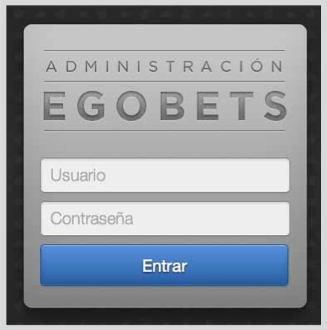
\includegraphics[width=\linewidth]{login}}
     \caption{Login}\label{Fig:Login1}
   \end{minipage}
   \begin {minipage}{0.49\textwidth}
     \frame{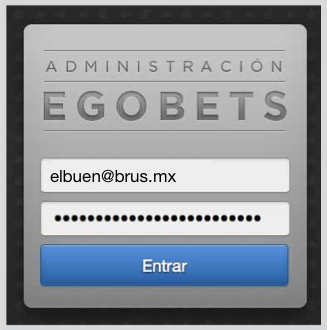
\includegraphics[width=\linewidth]{login-lleno}}
     \caption{Ingreso de datos}\label{Fig:Login2}
   \end{minipage}
\end{figure}

Al dar click en el botón de \underline{Entrar}, se habrá iniciado sesión, y se está habilitado para comenzar a trabajar.

Una vez que se haya terminado de usar el sistema, se debe cerrar la sesión, lo cual se puede hacer dando click sobre el botón de Salir. Véase figura~\ref{Fig:Logout}

\begin{figure}[!htb]\centering
   \begin {minipage}{0.49\textwidth}
     \frame{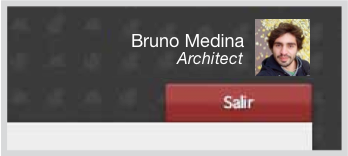
\includegraphics[width=\linewidth]{logout}}
     \caption[Cerrar Sesión]{Cerrar Sesión}\label{Fig:Logout}
   \end{minipage}
\end{figure}

Al hacerlo, se terminará de manera segura la sesión .
\section{Ingesta}
A través de este módulo se alimenta el sistema con la información necesaria para que la aplicación trabaje correctamente.

Lo elementos que se ingresan en este módulo son:

\begin{itemize}
\item Próximos partidos
\item Resultados de partidos anteriores
\item Estadísticas de los equipos en la temporada
\end{itemize}

Al entrar a esta sección, se encuentra un campo para seleccionar el tipo de ingesta que se quiere realizar, en este caso hay dos opciones:

\begin{itemize}
\item Partidos  
\item Equipos
\end{itemize}
Véase figura~\ref{Fig:ingesta}

\begin{figure}[!htb]\centering
   \begin {minipage}{0.8\textwidth}
     \frame{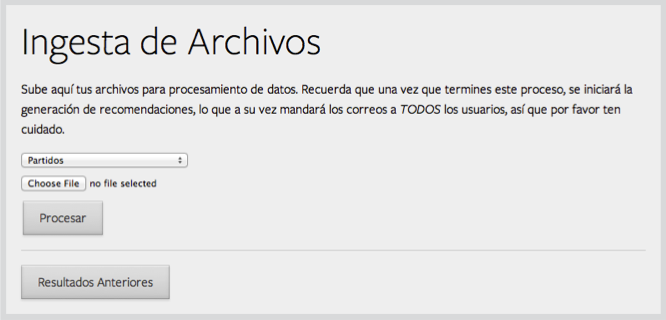
\includegraphics[width=\linewidth]{ingesta}}
     \caption[Subir y procesar archivos]{Subir archivos y procesarlos\footnotemark}
	 \label{Fig:ingesta}
   \end{minipage}
\end{figure}
\footnotetext{Toda la información referente a los archivos que se deben subir se encuentra en el~\ref{chap:archivos} }




\subsubsection{Partidos}
\begin{figure}[!htb]\centering
   \begin {minipage}{1\textwidth}
     \frame{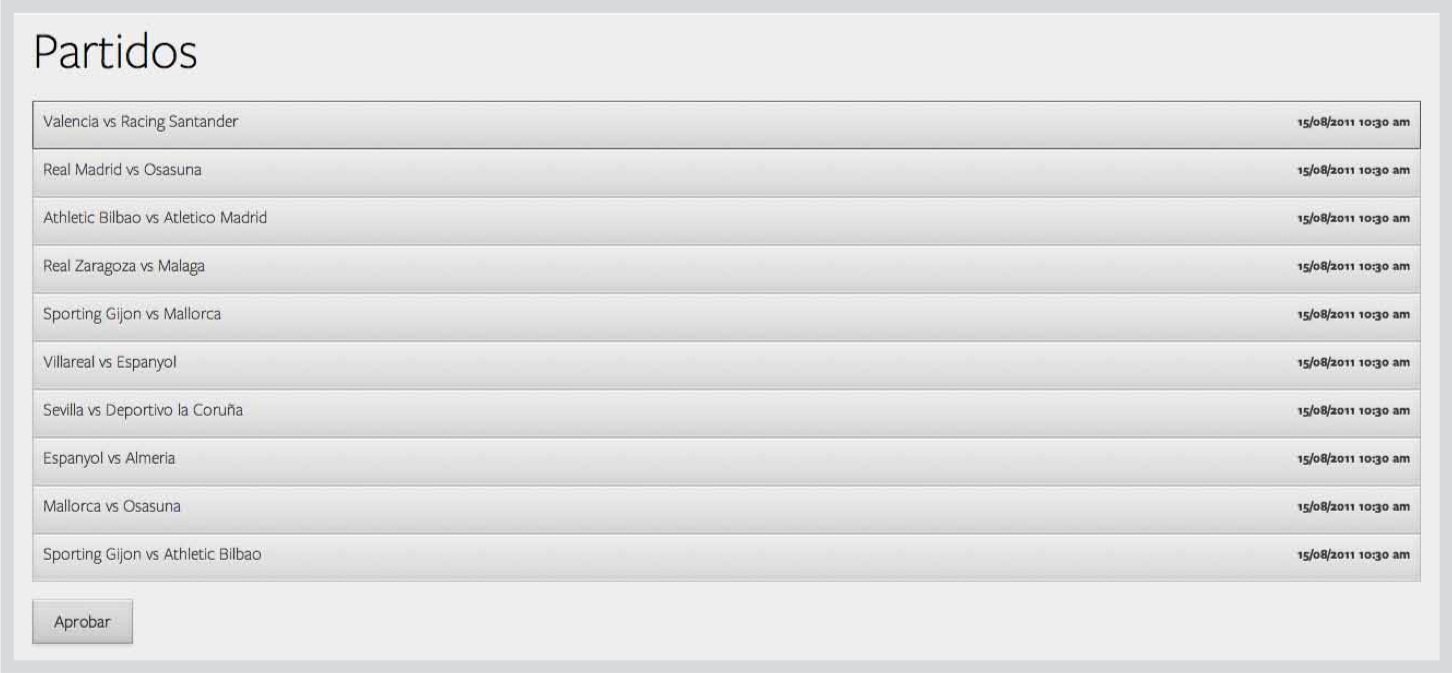
\includegraphics[width=\linewidth]{partidos}}
     \caption{Partidos procesados por el sistema}
	 \label{Fig:partidos}
   \end{minipage}
\end{figure}

Para subir la información de los partidos de la jornada que comienza, se selecciona del menú la opción de \textbf{Partidos}, y se presiona el botón \underline{Seleccionar archivo} donde se elige el archivo correspondiente.
Una vez seleccionado el archivo a ingestar y el tipo de datos que contiene, se oprime el botón de \underline{Procesar}, lo cual comienza el proceso de ingesta.\footnote{Una vez que comenzado el proceso de ingesta (ya sea de equipos ó partidos), se tienen sólo 10 minutos para verificar que los datos sean correctos. De no hacerlo, el sistema no procesará el archivo hasta que se suba nuevamente}

Con el archivo ya procesado, se puede verificar la interpretación que el sistema realizó del archivo. Se pueden observar en pantalla los siguientes datos:
\begin{itemize}
\item Identificador único y nombre del equipo local
\item Identificador único y nombre del equipo visitante
\item Marcadores de equipo local y visitante
\item Probabilidades de local, empate y visitante
\item Fecha en la que se llevará a cabo el partido
\end{itemize}

Si hay algún error en la información se puede presionar \underline{Cancelar} e intentarlo nuevamente, si la información es la correcta se oprime el botón de \underline{Aceptar}.


\subsubsection{Equipos}
\begin{figure}[!htb]\centering
   \begin {minipage}{1\textwidth}
     \frame{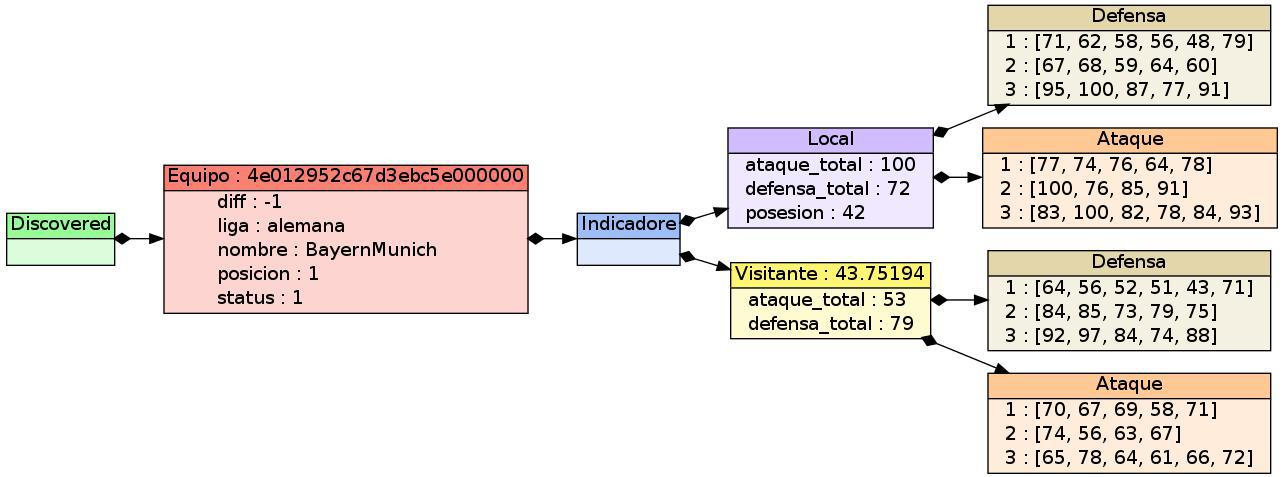
\includegraphics[width=\linewidth]{equipos}}
     \caption{Actualizando datos de los equipos}
	 \label{Fig:equipos}
   \end{minipage}
\end{figure}

Para la ingesta de datos de los equipos se selecciona la pestaña de \underline{Equipos} en la pestaña y luego se presiona el botón \textbf{Seleccionar archivo}.
Una vez que se seleccione el archivo a ingestar y el tipo de datos que contiene, se oprime el botón de \underline{Procesar}, para comenzar el proceso de ingesta.
Cuando el archivo termina de ser procesado el sistema presentará la interpretación del archivo, donde se podrán verificar los siguientes datos:
\begin{itemize}
\item Nombre del equipo
\item Indicadores de ataque y promedio de ataques:
	\begin{itemize}
		\item Medio Centro
		\item Delanteros
		\item Definición
	\end{itemize}
\item Indicadores de defensa y promedio de defensas:
	\begin{itemize}
		\item Medio centro,
		\item Defensa
		\item Portero
		\item Posesión
	\end{itemize}
\end{itemize}

Si hay algún error en la información se puede presionar \underline{Cancelar} e intentarlo nuevamente, si la información es la correcta se oprime el botón de \underline{Aceptar}.


\subsubsection{Resultados Anteriores}

Al dar clic en el botón de \underline{Resultados Anteriores} se pueden ver y modificar los resultados de los partidos de la semana pasada. En esta pantalla se actualizan los marcadores, al terminar se da click en \underline{Guardar Resultados}.

\begin{figure}[!htb]\centering
   \begin {minipage}{0.64\textwidth}
     \frame{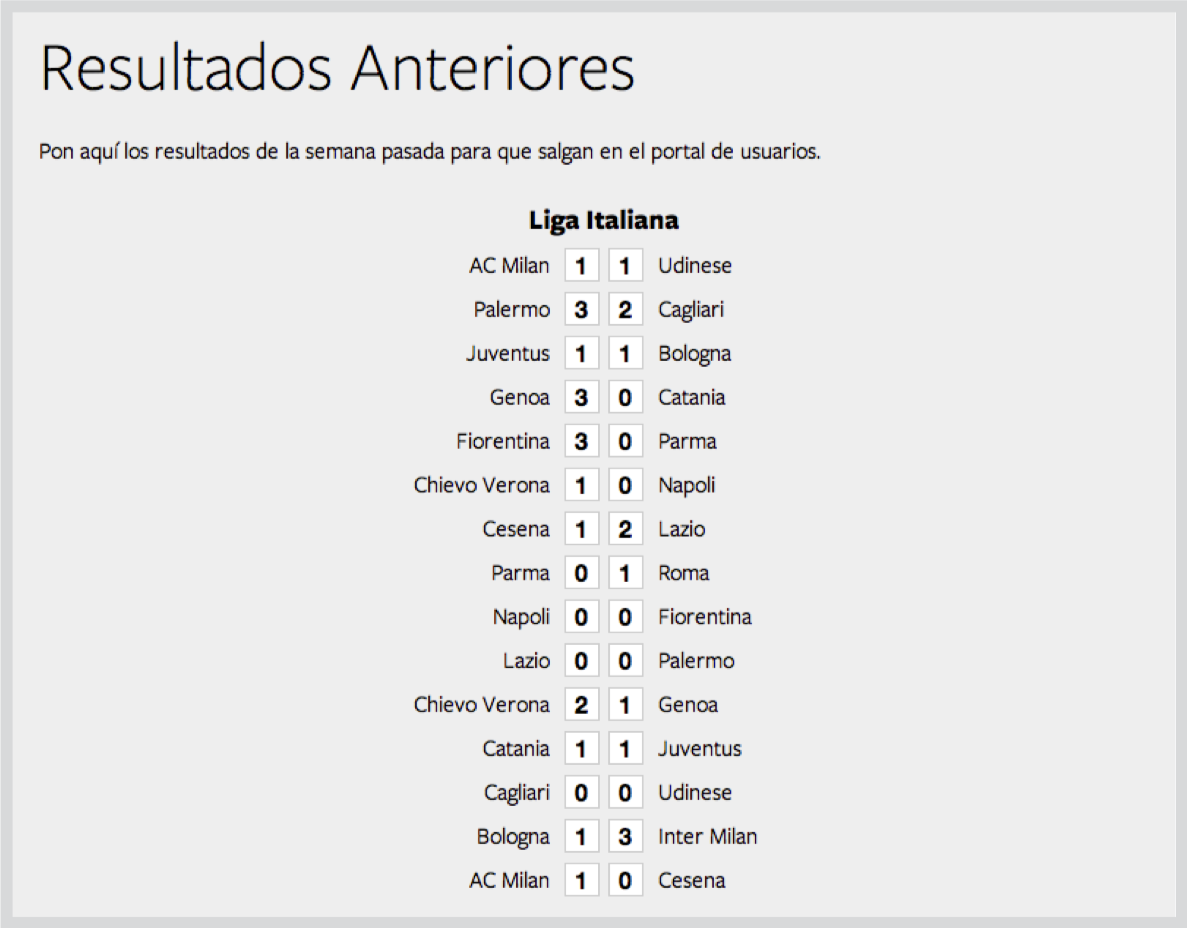
\includegraphics[width=\linewidth]{resultados-anteriores}}
     \caption[Actualizar resultados Anteriores]{Actualizando marcadores de la liga italiana}
	 \label{Fig:Resultados-anteriores}
   \end{minipage}
\end{figure}

Si el marcador de un partido que ya tenía resultado se deja en blanco no será modificado al guardar y se mostrará el resultado que tenía previamente.

\section{Usuarios}

Se muestran de quince en quince todos los usuarios inscritos a Egobets, para ver los siguientes quince usuarios se da click en el botón \underline{Siguiente}. Cada usuario tiene un botón de \underline{Detalles} y \underline{Eliminar}.
\begin{figure}[!htb]\centering
   \begin {minipage}{1\textwidth}
     \frame{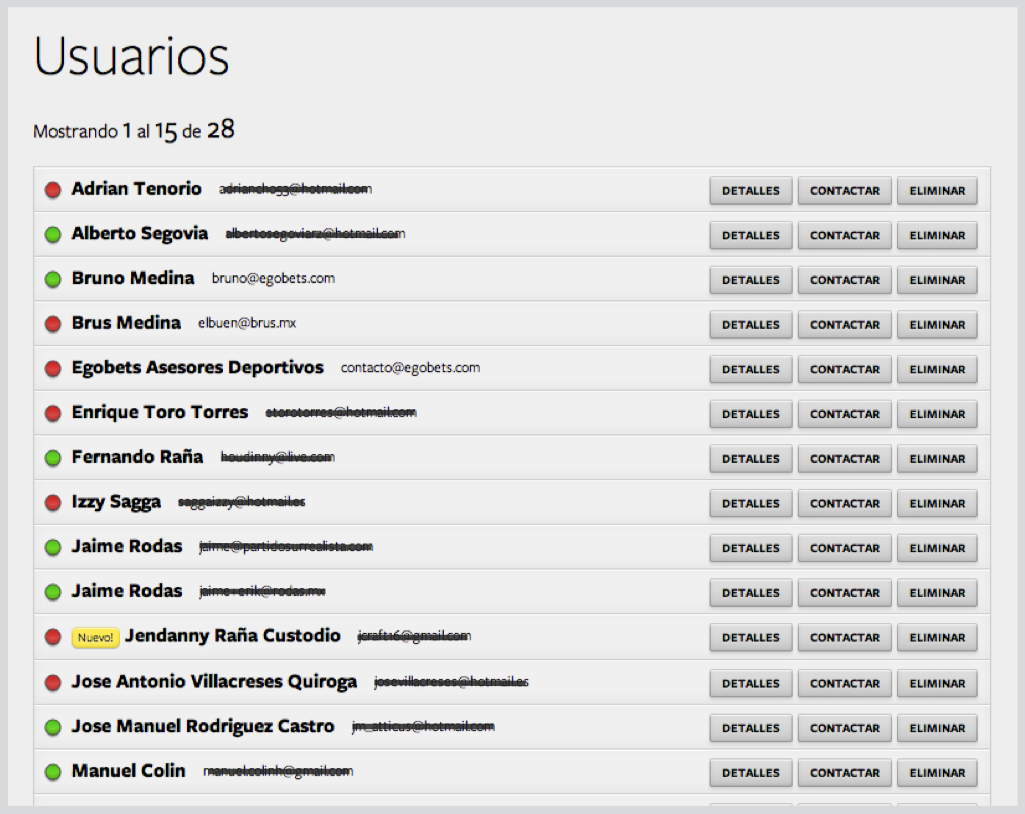
\includegraphics[width=\linewidth]{usuarios}}
     \caption{Listado de Usuarios}
	 \label{Fig:usuarios}
   \end{minipage}
\end{figure}

\subsubsection{Detalles de Usuario}

El botón Detalles en el listado presenta la información más detallada del usuario. Aquí se puede ver su información y preferencias:

\begin{figure}[!htb]\centering
   \begin {minipage}{1\textwidth}
     \frame{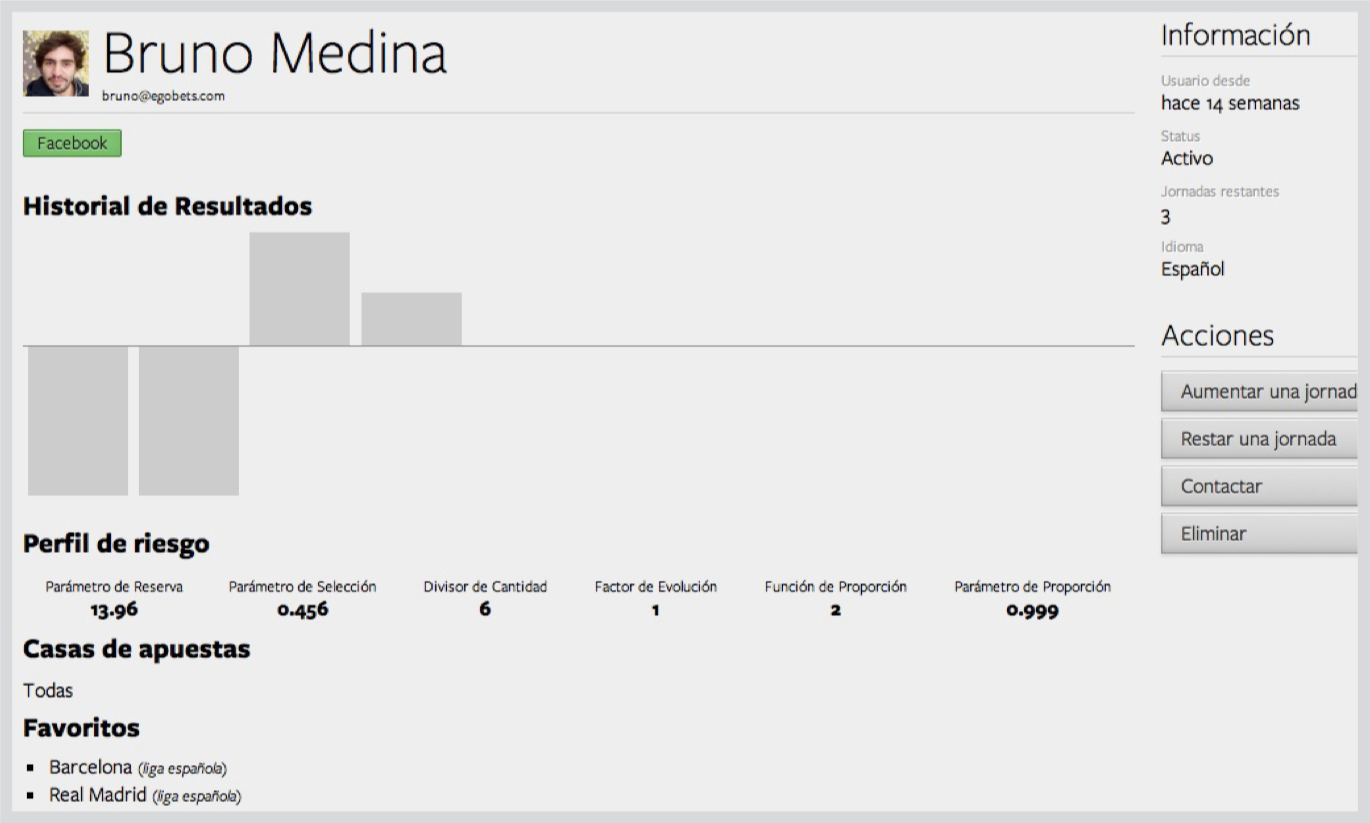
\includegraphics[width=\linewidth]{detalle-usuario}}
     \caption{Vista del detalle de usuario}
	 \label{Fig:Detalle-usuario}
   \end{minipage}
\end{figure}

\begin{itemize}
	\item \textbf{Historial.} Indica las últimas ganancias y pérdidas por jornada
	\item \textbf{Perfil de riesgo.} Despendiendo de la encuesta realizada por usuario se tiene su adversidad al riesgo.
	\item \textbf{Casas de apuesta.} En el sistema se tienen varias Casas que proporcionan distintos momios para los partidos.
	\item \textbf{Favoritos.} Los equipos favoritos del usuario
	\item \textbf{Transacciones realizadas.} Los últimos pagos realizados.
	\item \textbf{Usuario desde.} Tiempo que lleva como usuario de Egobets.
	\item \textbf{Estatus de actividad.} Al ser un sistema de paga los usuarios pagan por jornada para recibir la asesoría de apuestas.
		\begin{itemize}
			\item Activo: el usuarios está recibiendo recomendaciones.
			\item Inactivo: el usuario no está recibiendo recomendaciones.
		\end{itemize}
	\item \textbf{Jornadas restantes.} La cantidad de Jornadas que el usuario va seguir recibiendo asesorías.
	\item \textbf{Idioma.} En que lenguaje lee el portal el usuario (Inglés o Español)
\end{itemize}

\textbf{Acciones Administrativas}
\begin{itemize}
\item \textbf{Aumentar/Restar una Jornada.}
Una jornada le permite al usuario recibir la asesoría de los siguientes partidos.
Los administradores del sistema le pueden otorgar o quitar a los usuarios jornadas con tan solo click en el botón.

\item \textbf{Contactar.}
Permite al administrador enviar un correo desde su progama predeterminado de correo al usuario.

\item \textbf{Eliminar.} Todos los datos del usuario son eliminados del sistema.
\end{itemize}

\begin{figure}[!htb]\centering
   \begin {minipage}{0.5\textwidth}
     \frame{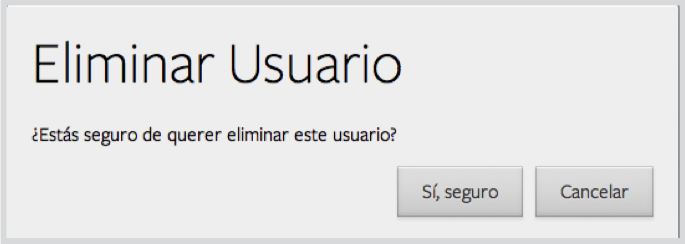
\includegraphics[width=\linewidth]{eliminar-usuario}}
     \caption[Confirmar la eliminación de un usuario]{Confirmar la eliminación de un usuario\footnotemark}
	 \label{Fig:Eliminar-usuario}
   \end{minipage}
\end{figure}

\footnotetext{La información de los usuarios eliminados no podrá ser rescatada.}

\section{Pagos}
Los pagos de los usuarios se cambian por la sugerencia de apuestas de una jornada. En esta sección se muestra un listado de las transacciones monetarias más recientes y su información general.

\begin{figure}[!htb]\centering
   \begin {minipage}{1\textwidth}
     \frame{\includegraphics[width=\linewidth]{Transacciones}}
     \caption{Listado con los últimos pagos realizados}
	 \label{Fig:Transacciones}
   \end{minipage}
\end{figure}

Los detalles de las transacciones son:
\begin{itemize}
	\item Fecha en la que la transacción se inicio.
	\item Número de transacción en la cuenta de PayPal de Egobets.
	\item Nombre y el correo del usuario que realiza la transacción, al dar clic sobre su nombre serán dirigidos a la información detallada de dicho usuario
	\item Cantidad de jornadas por las que se realiza la transacción
	\item Cantidad monetaria por la que se realiza la transacción
	\item Estatus de la transacción:
	\begin{itemize}
		\item Pendiente: se ha iniciado la transacción para la compra de jornadas, sin embargo aun no ha concluido.
		\item Pagada: se realizó exitosamente y las jornadas han sido agregadas al usuario.
	\end{itemize}
\end{itemize}

\section{Estadísticas}

Esta sección muestra las estadísticas y gráficas a los usuarios administrativos con información relevante de: ganancias y pérdidas de los usuarios, resultados de las predicciones, preferencias de los usuarios, pagos y partidos.

\subsubsection{Resultados Netos}

Indica el promedio de las ganancias y pérdidas de todos los usuarios en las últimas cinco jornadas, esta información se puede ver de manera porcentual o en cantidad neta.
Véase figura~\ref{Fig:mayor-ganancia}
\begin{figure}[!htb]\centering
   \begin {minipage}{0.4\textwidth}
     \frame{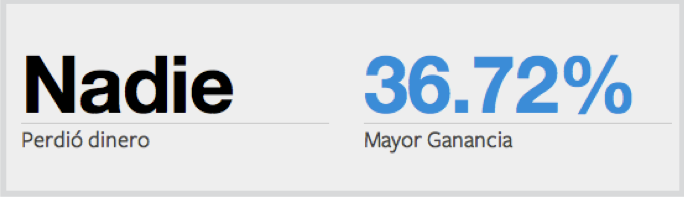
\includegraphics[width=\linewidth]{mayor-ganancia}}
     \caption{Ganancias y pérdidas de los usuarios}
	 \label{Fig:mayor-ganancia}
   \end{minipage}
\end{figure}


\textbf{Mayor Pérdida.}
Indica la mayor pérdida porcentual que se ha dado en la última jornada y al dar click presenta el perfil de dicho usuario.

\textbf{Mayor Ganancia.}
Indica la ganancia porcentual mayor que se ha dado en la última jornada y al dar click presenta el perfil de dicho usuario.


\subsubsection{Usuarios y sus Datos}

\textbf{Total.} Número total de usuarios registrados y al dar click presenta la sección de \underline{Usuarios}.

\textbf{Nuevos.} Número de usuarios registrados recientemente y al dar click presenta la sección de \underline{Usuarios}.

Véase figura~\ref{Fig:nuevos-usuarios}
\begin{figure}[!htb]\centering
   \begin {minipage}{0.4\textwidth}
     \frame{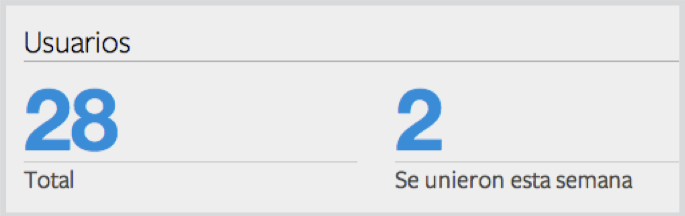
\includegraphics[width=\linewidth]{nuevos-usuarios}}
     \caption{Usuarios recién inscritos}
	 \label{Fig:nuevos-usuarios}
   \end{minipage}
\end{figure}

Además, el sistema muestra la siguiente información general, porcentaje de usuarios que:
\begin{itemize}
	\item Usan Facebook para conectarse a Egobets
	\item Usan apuestas dobles
	\item Usan reserva
	\item Ven Egobets en inglés
	\item Se encuentran activos.
\end{itemize}
Véase figura~\ref{Fig:graficas-usuarios}
\begin{figure}[!htb]\centering
   \begin {minipage}{1\textwidth}
     \frame{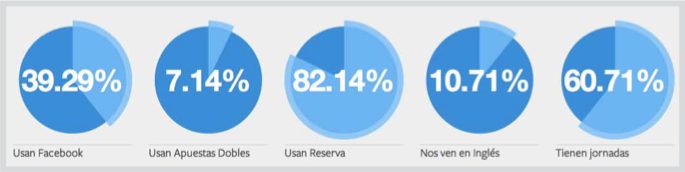
\includegraphics[width=\linewidth]{graficas-usuarios}}
     \caption{Datos estadísticos de los usuarios}
	 \label{Fig:graficas-usuarios}
   \end{minipage}
\end{figure}
 
\subsubsection{Pagos Recibidos}

\begin{figure}[!htb]\centering
   \begin {minipage}{0.5\textwidth}
     \frame{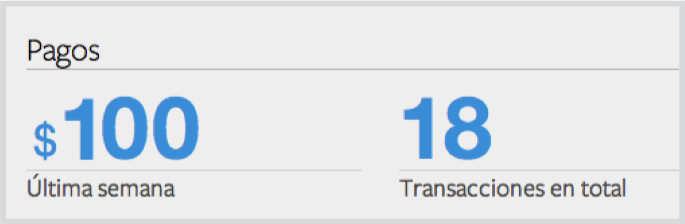
\includegraphics[width=\linewidth]{ultimos-pagos}}
     \caption{Pagos más recientes}
	 \label{Fig:ultimos-pagos}
   \end{minipage}
\end{figure}

\textbf{Última Semana.}
Se representan las ganancias monetarias que obtenidas durante la última semana. Al dar click se muestra la sección de \textbf{Pagos}.

\textbf{Transacciones en total.}
Indica el número de transacciones que se han realizado durante todo el tiempo del sistema.

\subsubsection{Partidos y Predicciones}

\begin{figure}[!htb]\centering
   \begin {minipage}{0.5\textwidth}
     \frame{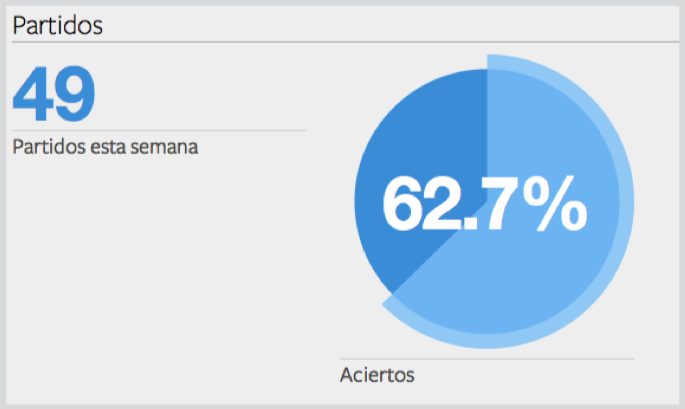
\includegraphics[width=\linewidth]{partidos-acertados}}
     \caption{Partidos acertados}
	 \label{Fig:partidos-acertados}
   \end{minipage}
\end{figure}

\textbf{Aciertos}
Presenta la cantidad de partidos de esta semana y al dar clic nos lleva a la sección de \underline{Ingesta}.

\textbf{Aciertos}
Representan con una gráfica la cantidad de aciertos obtenidos en las predicciones hechas en partidos pasados. Al presionarla se dirige el navegador a los \underline{Resultados Anteriores} dentro de la sección de \underline{Ingesta}.

\section{Correos}

En esta sección se puede enviar correos a un subconjunto de usuarios registrados en Egobets. Los mensajes deberán ser escritos en Español y en Inglés para que el correo recibido dependa del lenguaje elegido por el usuario al crear su cuenta. Los grupos de usuarios con los que nos se puede comunicar son:

\begin{itemize}
	\item Todos los usuarios
	\item Usuarios activos: aquellos que tienen jornadas pagadas
	\item Usuarios inactivos: aquellos que ya no tienen jornadas pagadas
	\item Usuarios registrados: aquellos que se registraron pero no han confirmado su correo
\end{itemize}
Véase figura~\ref{Fig:correos}

\begin{figure}[!htb]\centering
   \begin {minipage}{0.8\textwidth}
     \frame{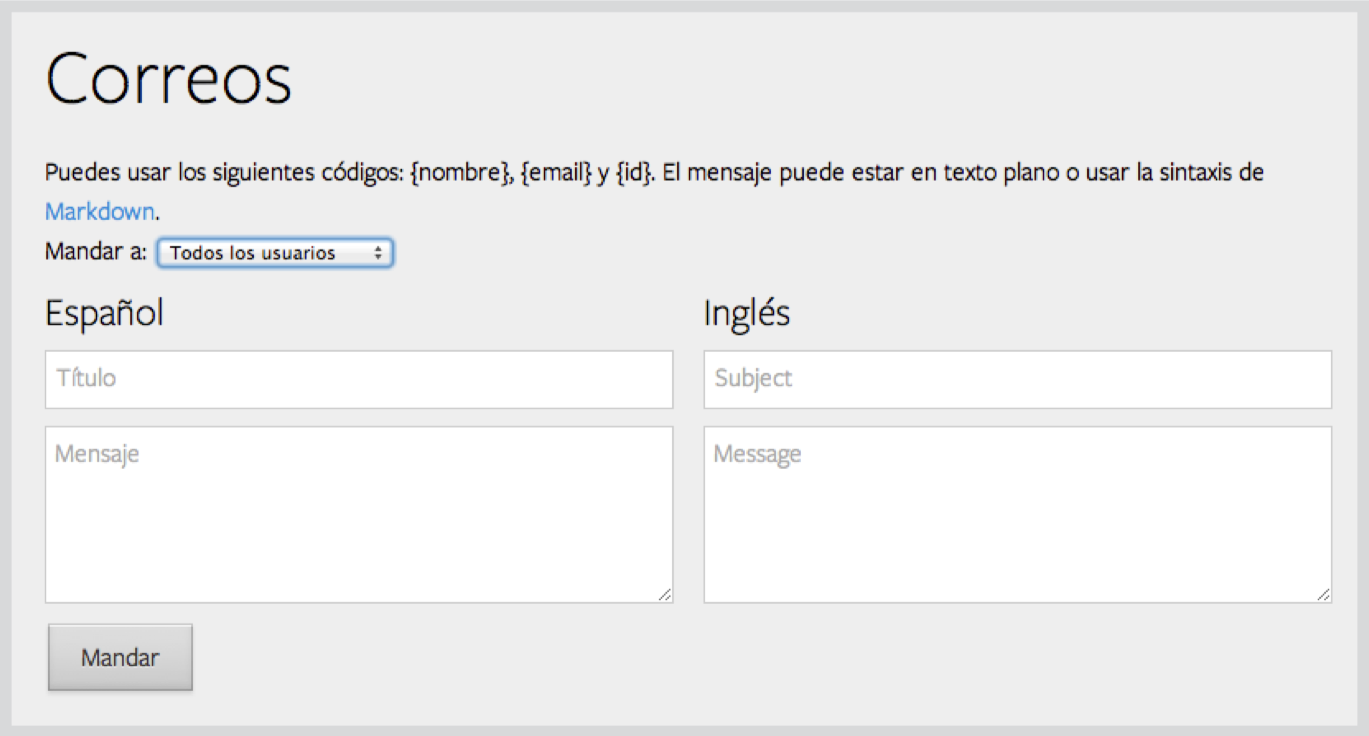
\includegraphics[width=\linewidth]{correos}}
     \caption{Comunicación con los usuarios}
	 \label{Fig:correos}
   \end{minipage}
\end{figure}

Para redactar los textos, se debe usar la sintaxis de Markdown\footnote{El hipervínculo de \underline{Markdown} redirige a una página dónde se puede aprender sobre el uso de esta sintaxis.}.
Se pueden usar textos de reemplazo cuándo se quieran personalizar los mensajes, para esto basta con utilizar las palabras clave: \{nombre\}, \{correo\} y \{id\}, las cuales el sistema sustituirá, al momento de mandar el correo, por los valores correspondientes para cada usuario.



\chapter{Preguntas frecuentes}\label{chap:faq}

En este apéndice se encuentra el FAQ\footnote{El acrónimo significa: \textbf{Preguntas Frecuentes}. En inglés la abreviación corresponde a: \textbf{``Frequently Asked Questions''}.} del portal público \emph{``\emph{Egobets.com}''}, esta información busca cubrir las dudas que pudieran tener los usuarios con respecto a la operación del portal. Es importante recalcar que también tienen un proposito promocional.

\section{Preguntas del portal en general}
\begin{itemize}
\item \textbf{¿Qué es Egobets.com?}


Egobets es el mejor sistema de recomendación personalizada de apuestas deportivas para fútbol europeo en Internet.

\item \textbf{¿Qué servicios ofrece Egobets.com?}


Algunos de los servicios son los siguientes:
\begin{enumerate}
	\item \emph{Recomendación personalizada de apuestas en fútbol:} Cada persona es diferente y debe ser tratada de forma única, en Egobets se determina el perfil de riesgo de cada usuario mediante una encuesta y se le recomienda apuestas a su medida, de tal forma que pueda obtener ganancias y sentirse cómodo al mismo tiempo.
	\item \emph{Pronósticos:} Para cada partido se proporcionan, entre otros: marcador final más probable, resultado más probable y el nivel de posesión de balón de cada equipo.
	\item \emph{Estadísticas:} A través de éstas se pueden analizar las fortalezas y debilidades de los equipos favoritos del usuario.
\end{enumerate}

\item \textbf{¿Por qué usar el servicio de Egobets.com?}


Algunas de las ventajas son:
\begin{enumerate}
	\item Es el único servicio de apuestas personalizadas del mercado.
	\item Al mostrar los momios de las casas de apuestas más populares del mercado, se presenta en las recomendaciones el rendimiento más grande del mercado.
	\item Los precios por el servicio son los más competitivos y se ofrece un servicio de mayor calidad que cualquier otro portal de asesoría de apuestas.
\end{enumerate}

\end{itemize}



\section{Preguntas del tablero}
\begin{itemize}

\item \textbf{¿Qué es el tablero y para qué sirve?}


El tablero es la página principal para el usuario de \emph{Egobets.com}. En el tablero se presenta la recomendación de la semana:
1.	Barra de ingreso.
2.	Los partidos en que se apostará: el partido, el resultado a apostar, la cantidad de dinero a apostar, el momio ofrecido y la casa de apuestas que ofrece tal momio.
3.	La gráfica de valor esperado.
\item \textbf{¿Por qué se pregunta la cantidad de dinero a apostar?}


Para poder indicar en la recomendación la cantidad de dinero a apostar, si el recuadro se deja en blanco entonces la cantidad de dinero a apostar se presentará como porcentaje.

\item \textbf{¿Qué representa la primera barra?}


Representa la cantidad de dinero total del cliente: cada cuadro es la cantidad de dinero que se recomienda apostar en un partido, al poner el apuntador arriba de un cuadro se iluminará el partido correspondiente. La parte gris representa el dinero que no se apostará en la semana, es decir, la reserva.

\item \textbf{¿Por qué al principio de cada jornada se preguntn la cantidad de dinero antes de apostar y después de apostar?}


En \emph{Egobets.com} se le da seguimiento a cada uno de nuestros clientes. Con esta información se puede monitorear la evolución del ingreso y así dar las recomendaciones de acuerdo al nivel de ganancias o pérdidas. Es importante que esta información sea verdadera para poder brindar el mejor servicio posible.

\item \textbf{¿Qué es la gráfica de últimos resultados que se muestra en el menú de arriba?}


Es una representación gráfica del porcentaje de ganancias que el cliente ha tenido en las últimas semanas. Un click la agranda.

\item \textbf{¿Se pueden hacer recomendaciones de resultados que no sean los más probables?}


Sí, depende del perfil de riesgo y de lo que pague la casa de apuestas en tal partido. En algunas ocasiones es recomendable apostar en contra del favorito si el pago es suficientemente grande. Si se tiene activado el sistema en contra de favoritos (en el menú perfil) o si el perfil es muy agresivo se presentarán muchas recomendaciones de este tipo. 
\end{itemize}

\section{Gráfica de valor esperado}
\begin{itemize}
\item \textbf{¿Qué es la gráfica de valor esperado?}


La gráfica de valor esperado es una herramienta visual que permite ver cuáles son los posibles resultados de la recomendación de la semana. En \emph{Egobets.com} se conoce que todas las apuestas tienen un riesgo y mediante esta gráfica se puede cuantificar: Cada barra representa la probabilidad de que se gane o pierda la cantidad indicada debajo de ella, mientras más grande sea la barra mayores probabilidades hay de que tal resultado ocurra.

\item \textbf{¿Por qué aparecen barras en números negativos?}


La parte negativa de la gráfica representa el riesgo de la apuesta (o probabilidad de perder dinero). Sin embargo, las recomendaciones del sistema están calculadas de tal forma que la parte positiva de la gráfica sea mayor que la parte negativa, es decir, que en el mediano plazo se puedan obtener ganancias aunque haya habido algunas semanas con pérdidas.

\end{itemize}

\section{Preguntas del menú mis equipos}
\begin{itemize}

\item \textbf{¿Qué equipos aparecen en la sección de mis equipos?}


En esta sección aparecen todos los equipos que hayas marcado como favoritos. Para marcar a un equipo como favorito debes acceder al menú de ligas, seleccionar la liga correspondiente al equipo y marcar a tal equipo como favorito haciendo click en la estrella al lado de su nombre.

\item \textbf{¿Qué ventajas tiene marcar un equipo como favorito?}


Poder tener acceso a las estadísticas de ese equipo de manera más rápida.
\end{itemize}

\section{Preguntas del menú de ligas}
\begin{itemize}

\item \textbf{¿Cuáles son las ligas que presenta \emph{Egobets.com}?}


Inglesa, española, francesa, italiana y alemana.

\item \textbf{¿Por qué el orden de la tabla en cada liga no es el orden oficial en la tabla de posiciones?}


En \emph{Egobets.com} se presentan los equipos mediante un power ranking. Con base en las estadísticas de los partidos y dados sus resultados, se pronostica cuál será la tabla de posiciones al finalizar dicha liga.

\item \textbf{¿Por qué las primeras cinco semanas de cada liga la tabla está ordenada de acuerdo a la tabla de posiciones del año pasado?}


Para las primeras cinco semanas no se tiene información suficiente para poder realizar un power ranking, sin embargo, a partir de la sexta semana la información presentada será de acuerdo al power ranking calculado.

\item \textbf{¿Qué información se presenta en la tabla de las ligas?}


En orden de aparición: Una estrella indicando si el equipo está o no marcado como uno de los favoritos, la posición en el power ranking, el nombre del equipo, el índice de ataque general del equipo, el índice de defensa general del equipo y por último el cambio dentro de la tabla de power ranking.

\item \textbf{¿Qué información se ofrece en la sección de cada equipo y cómo interpretarla?}


Se presentan las estadísticas del equipo, del lado izquierdo como local y del lado derecho como visitante:
\begin{enumerate}

\item Índice de ataque general: Con calificación de una a cinco estrellas o de uno a diez (abajo). Representa la capacidad general del equipo para atacar.
\item Índices de medio centro, delanteros y definición: Con una calificación de cero a cien. Representan la capacidad de controlar el medio centro, de atacar a portería y de precisión de los tiros, respectivamente.
\item Índice de defensa general: Con calificación de una a cinco estrellas o de uno a diez (abajo). Representa la capacidad general del equipo para defender.
\item Índices de medio centro, defensas y portero: Con una calificación del cero a cien. Representan la capacidad de defender en el centro, de los defensas y del portero, respectivamente.
\item Al hacer click en las variables mencionadas en 2 o 4 se tienen acceso a la evolución de tales variables desde el minuto 0 hasta el 90 de un partido.
\end{enumerate}

Por último, se presentan los partidos que tiene tal equipo en la semana.

\end{itemize}

\section{Preguntas del menú de partidos}
\begin{itemize}

\item \textbf{¿A qué información tengo acceso a través del menú de partidos de la semana?}


A resultados de la jornada anterior y a pronósticos de la jornada actual:
\begin{enumerate}

	\item \emph{Resultados de la jornada anterior:} Se presenta el partido, el marcador real, el marcador pronosticado y el resultado pronosticado. Esto con el fin de que los usuarios puedan comparar lo pronosticado y lo que en verdad ocurrió.
	\item \emph{Pronósticos de la jornada actual:} Se presenta el partido, el resultado pronosticado (o favorito), el marcador pronosticado y la fecha del encuentro. Además al poner el apuntador encima de un partido se presenta el grado de confiabilidad del pronóstico.
\end{enumerate}

Además para cada tabla se pueden presentar los resultados de una liga en particular al seleccionarla en el recuadro de arriba.

\item \textbf{¿Por qué algunos partidos aparecen de otro color en la tabla?}


Esos son los partidos en los cuáles el sistema te ha recomendado apostar. Para ver la recomendación debes acceder al menú tablero.

\item \textbf{¿Qué es el grado de confiabilidad?}


Es el nivel de certeza que se tiene del pronóstico del resultado del partido (local, empate o visitante), se mide de cero a cinco estrellas. A mayor cantidad de estrellas es más posible que ocurra el resultado pronosticado.

\item \textbf{¿Qué información se presenta en la sección de un partido?}


El pronóstico del partido y las estadísticas de cada equipo:
\begin{enumerate}

\item Pronósticos: Se pronostica el marcador final, la posesión del balón y el ganador del encuentro. Al poner el apuntador sobre el resultado más probable aparece el grado de confiabilidad del pronóstico.
\item Estadísticas: Se presentan las mismas estadísticas que en la sección de cada equipo, del lado derecho las del equipo local y del lado izquierdo las del visitante, para hacerlo fácil de comparar.
\end{enumerate}

\end{itemize}

\section{Preguntas del menú del perfil}
\begin{itemize}

\item \textbf{¿Qué puede hacer el usuario a través del menú del perfil?}


Se pueden realizar las siguientes acciones:
\begin{enumerate}

\item Cambiar el idioma: Inglés o español.
\item Indicar si se desea o no el sistema de apuestas en contra de favoritos: Explicación en las siguientes preguntas.
\item Cambiar las casas de apuestas: El usuario puede indicar en qué casas de apuestas estás inscrito y las recomendaciones se harán considerando los momios que éstas ofrezcan. Si no se está inscrito a alguna de las listadas se recomienda dejar la opción de todas activa.
\item Hacer pagos: Se puede incrementar la cantidad de jornadas de recomendaciones.
\item Cambiar contraseña.
\item Cambiar perfil de riesgo: El usuario puede volver a tomar la encuesta de riesgo para generar recomendaciones a su medida.
\item Conectar con Facebook: El usuario ligar su cuenta de Facebook con la de \emph{Egobets.com}.
\end{enumerate}

Los cambios en preferencias, casas de apuesta o el perfil de riesgo; se verán reflejados hasta un día después.
\end{itemize}

\section{Sistema en contra de favoritos}
\begin{itemize}

\item \textbf{¿Qué es el sistema en contra de favoritos?}


Es un sistema para jugadores que buscan riesgo moderado o alto en el cual se determina en cuáles partidos apostar en contra del equipo favorito.

\item \textbf{¿Cómo funciona?}


Se analiza cada partido por separado mediante un modelo probabilístico que encuentra los equipos favoritos que no son tan fuertes como lo creen las casas de apuesta o la opinión popular.

\item \textbf{¿Qué son las apuestas dobles y por qué se usan en este sistema?}


Una apuesta doble es cuando se apuesta en uno de los siguientes resultados: local-empate, empate-visitante o local-visitante. El sistema en contra de favoritos recomienda apostar en los resultados contrarios al favorito del partido, por ejemplo, si el favorito de un partido es local se le podrá recomendar la apuesta empate-visitante para que la probabilidad de acertar no sea tan baja.

\item \textbf{¿Por qué apostar en contra del favorito?}


Apostar en contra de un equipo favorito paga más que apostar a lo “seguro”. En fútbol no es raro que equipos ordinarios le ganen a equipos extraordinarios y es en esas ocasiones donde se puede ganar mucho dinero.

\end{itemize}

\section{Con respecto a los pagos}
\begin{itemize}

\item \textbf{¿Cómo se pueden comprar más jornadas?}


A través del menú de arriba donde se indican la jornadas restantes o a través del menú de pagos en perfil.

\item \textbf{¿Qué información se presenta en la sección de pagos?}


Se presentan los paquetes disponibles y el historial de pagos realizados por el usuario. ¡Contrata hasta 10 jornadas y recibe el mejor descuento!

\item \textbf{¿Qué formas de pago tiene \emph{Egobets.com}?}


Pago con tarjetas de crédito, con cuenta paypal o por depósito bancario. Para cualquier reclamación con el sistema de pagos favor de contactar a paypal. Para cualquier devolución del dinero favor de contactar a contacto@\emph{Egobets.com}.com indicando el motivo y se te contestará a la mayor brevedad posible.
\end{itemize}

\section{Con respecto a los perfiles de riesgo}
\begin{itemize}

\item \textbf{¿De qué sirve el perfil de riesgo y cómo lo calculan?}


El perfil de riesgo sirve para poder personalizar la asesoría de apuestas y se calcula a través de las respuestas proporcionadas en la encuesta de perfil de riesgo.

\item \textbf{¿Se puede cambiar el perfil de riesgo?}


Lo puedes cambiar tantas veces como desees desde el menú de perfil, sin embargo, el cambio tarda 24 horas en aparecer en el sistema.
\item \textbf{¿Es obligatorio contestar la encuesta de riesgo?}


 Sí pues es la única forma en el que el sistema puede otorgarte un perfil.

\item \textbf{¿Cuál es la diferencia entre los diferentes perfiles de riesgo?}


De forma genérica hay tres perfiles de riesgo:
\begin{enumerate}
	\item Agresivo: Toma riesgos altos para poder obtener la mayor cantidad de ganancias posibles en el corto plazo. 
	\item Conservador: Apuesta a lo más seguro para proteger su dinero lo más posible, busca ganancias al largo plazo.
	\item Moderado: Término medio entre agresivo y conservador.
\end{enumerate}

\textbf{¿Cuál perfil de riesgo conviene más?}


Eso depende de los gustos personales del cliente. Para cualquier perfil de riesgo se harán recomendaciones que le permitan tener la mayor cantidad de ganancias posibles y al mismo tiempo que le hagan sentir cómodo al apostar.
\end{itemize}

\section{Con respecto a la reserva}
\begin{itemize}

\item \textbf{¿Cuánto dinero debería apostar el cliente esta semana?}


En \emph{Egobets.com} se entiende que cada persona es diferente, que cada apuesta es diferente y debe ser analizada de forma individual, por eso se ha desarrollado el sistema de reservas que determina cuánto dinero apostar en la recomendación de la semana.

\item \textbf{¿Qué es la reserva y para qué sirve?}


La reserva es la cantidad de dinero que no se apostará, sirve para poder seguir apostando en semanas posteriores en el caso en que se lleguen a tener pérdidas.

\item \textbf{¿Cómo funciona el sistema de reservas?}


Se toman en cuenta tres factores: la volatilidad de la apuesta, la ganancia esperada de ésta y el nivel de riesgo deseado del cliente. Se combina esta información en un modelo probabilístico que proporciona la cantidad a apostar. Mediante este sistema se busca de proteger al cliente de pérdidas potenciales.

Beneficios:
\begin{enumerate}

	\item Protege su dinero de pérdidas potenciales.
	\item Permite recuperarse con mayor velocidad de semanas con pérdidas.
	\item Permite dar una estructura de fondo de inversión a las apuestas al obtener un sistema de interés compuesto.

\end{enumerate}

Costos:
\begin{enumerate}
	\item Se restringe la cantidad de ganancias a corto plazo.
\end{enumerate}

Es un sistema a largo plazo, no se recomienda a personas que desean incurrir en riesgos elevados en beneficio de la posibilidad de obtener mayores ganancias.

\end{itemize}




\thispagestyle{empty}

\addtocontents{toc}{\vspace{2em}} % Agrega espacio en la toc

%----------------------------------------------------------------------------------------
%	Bibliografía
%----------------------------------------------------------------------------------------

\backmatter
\printbibliography

\end{document}  